% Author: Alfredo Sánchez Alberca (asalber@gmail.com)
\section{Frequency distributions: Tabulation and charts}

\mode<presentation>{
%---------------------------------------------------------------------slide----
\begin{frame}
\frametitle{Frequency distribution: Tabulation and charts}
\tableofcontents[sectionstyle=show/hide,hideothersubsections]
\end{frame}
}


%---------------------------------------------------------------------slide----
\begin{frame} 
\frametitle{Descriptive Statistics}
Descriptive Statistics is the part of Statistics in charge of representing, analysing and summarizing the information
contained in the sample.

After the sampling process, is the next step in every statistical study and usually consists of:
\begin{enumerate}
\item Classify, group and sort the data of the sample.
\item Tabulate and plot data according to their frequencies.
\item Calculate numerical measures that summarize the information contained in the sample (\emph{sample statistics}).
\end{enumerate} 

It has no inferential power $\Rightarrow$ \alert{\emph{Do not generalize to the population!}} 
\end{frame}


\subsection{Frequency distribution}
%---------------------------------------------------------------------slide----
\begin{frame}
\frametitle{Sample classification}
The study of a statistical variable starts measuring the variable in the individuals of the sample and classifying the
values.

There are two ways of classifying data:
\begin{description}
\item[Non-grouping] Sort values from lowest to highest value (if there is an order).
Used with qualitative variables and discrete variables with few distinct values.
\item[Grouping] Group values in intervals (classes) and sort them from lowest to highest intervals. 
Used with continuous variables and discrete variables with many distinct values. 
\end{description}
\end{frame}


%---------------------------------------------------------------------slide----
\begin{frame}
\frametitle{Sample classification}
$X=$Height
\begin{center}
\scalebox{0.6}{% Autor: Alfredo Sánchez Alberca (email:asalber@ceu.es)
% Charts that shows the purpose of Statistics
\begin{tikzpicture}[every label/.style={text=color1}]
\node (sample) at (0,8) {\includegraphics[height=4cm]{img/descriptive/sample.png}}; 
\pause
\node (ordered-sample) at (0,0) {\includegraphics[height=4cm]{img/descriptive/ordered_sample.png}};
\node at (0,4) [fill=color2,single arrow,shape border rotate=270,minimum height=3cm,text=white, minimum width=4cm]{\huge
\ Classify\ \phantom{}};
\end{tikzpicture} }
\end{center}
\end{frame}


%---------------------------------------------------------------------slide----
\begin{frame}
\frametitle{Frequency count}
$X=$Height
\begin{center}
\scalebox{0.6}{% Autor: Alfredo Sánchez Alberca (email:asalber@ceu.es)
% Charts that shows the purpose of Statistics
\begin{tikzpicture}[every label/.style={text=color1}]
\node at (0,8) {\includegraphics[height=4cm]{img/descriptive/ordered_sample.png}}; 
\pause
\node at (0,0) {\includegraphics[height=4cm]{img/descriptive/sample_frequencies.png}};
\node at (0,4) [fill=color1,single arrow,shape border rotate=270,minimum height=3cm,text=white, minimum
width=4cm, align=center]{\huge Frequency\\ \huge count};
\end{tikzpicture} }
\end{center}
\end{frame}


%---------------------------------------------------------------------slide----
\begin{frame}
\frametitle{Sample frequencies}
\begin{definition}[Sample frequencies]
Given a sample of $n$ values of a variable $X$, for every value $x_i$ of the variable
is defined 
\begin{itemize}
\item \structure{Absolute frequency $n_i$}: Is the number of times that value $x_i$ appears in the sample.
\item \structure{Relative frequency $f_i$}: Is the proportion of times that value $x_i$ appears in the sample.
\[
f_i = \frac{n_i}{n}
\]
\item \structure{Cumulative absolute frequency $N_i$}: Is the number of values in the sample less than or equal to
$x_i$.
\[
N_i = n_1 + \cdots + n_i
\]
\item \structure{Cumulative relative frequency $F_i$}: Is the proportion of values in the sample less than or equal to
$x_i$.
\[
F_i = \frac{N_i}{n}
\]
\end{itemize}
\end{definition}
\end{frame}


%---------------------------------------------------------------------slide----
\begin{frame}
\frametitle{Frequency table}
The set of values of a variable with their respective frequencies is called \structure{\textbf{frequency distribution}}
of the variable in the sample, and it is usually represented as a \structure{\textbf{frequency table}}.
\begin{center}
\begin{tabular}{|>{\centering}p{1.8cm}|>{\centering}p{1.8cm}|>{\centering}p{1.8cm}|>{\centering}p{1.8cm}|p{1.8cm}<{\centering}|}
\hline
\structure{$X$ values} & \structure{Absolute frequency} & \structure{Relative frequency} & \structure{Cumulative
absolute frequency} & \structure{Cumulative relative frequency} \\
\hline
$x_1$ & $n_1$ & $f_1$ & $N_1$ & $F_1$\\
$\vdots$ & $\vdots$ & $\vdots$ & $\vdots$ & $\vdots$\\
$x_i$ & $n_i$ & $f_i$ & $N_i$ & $F_i$\\
$\vdots$ & $\vdots$ & $\vdots$ & $\vdots$ & $\vdots$\\
$x_k$ & $n_k$ & $f_k$ & $N_k$ & $F_k$\\
\hline
\end{tabular}
\end{center}
\end{frame}


%---------------------------------------------------------------------slide----
\begin{frame}
\frametitle{Frequency table}
\framesubtitle{Example of quantitative variable and non-grouped data}
The number of children in 25 families are:
\begin{center}
1, 2, 4, 2, 2, 2, 3, 2, 1, 1, 0, 2, 2, \\
 0, 2, 2, 1, 2, 2, 3, 1, 2, 2, 1, 2
\end{center}
The frequency table for the number of children in this sample is 
\[
\setlength\arraycolsep{3mm}
\setlength\arrayrulewidth{0.5pt}
\begin{array}{rrrrr}
\hline
x_i & n_i & f_i & N_i & F_i\\
\hline
0 & 2 & 0.08 & 2 & 0.08\\
1 & 6 & 0.24 & 8 & 0.32\\
2 & 14 & 0.56 & 22 & 0.88\\
3 & 2  & 0.08 & 24 & 0.96\\
4 & 1 & 0.04 & 25 & 1 \\
\hline
\sum & 25 & 1 \\
\hline
\end{array}
\]
\end{frame}


%---------------------------------------------------------------------slide----
\begin{frame}
\frametitle{Frequency table}
\framesubtitle{Example of quantitative variable and grouped data}
The heights (in cm) of 30 students are:
\begin{center}
179, 173, 181, 170, 158, 174, 172, 166, 194, 185,\\
162, 187, 198, 177, 178, 165, 154, 188, 166, 171,\\
175, 182, 167, 169, 172, 186, 172, 176, 168, 187.
\end{center}
The frequency table for the height in this sample is
\[
\setlength\arraycolsep{3mm}
\setlength\arrayrulewidth{0.5pt}
\begin{array}{rrrrr}
\hline
\multicolumn{1}{c}{x_i} & \multicolumn{1}{c}{n_i} & \multicolumn{1}{c}{f_i} & \multicolumn{1}{c}{N_i} & \multicolumn{1}{c}{F_i}\\
\hline
(150,160] & 2 & 0.07 & 2 & 0.07\\
(160,170] & 8 & 0.27 & 10 & 0.34\\
(170,180] & 11 & 0.36 & 21 & 0.70\\
(180,190] & 7  & 0.23 & 28 & 0.93\\
(190,200] & 2 & 0.07 & 30 & 1 \\
\hline
\sum & 30 & 1 \\
\hline
\end{array}
\]
\end{frame}


%---------------------------------------------------------------------slide----
\begin{frame}
\frametitle{Classes construction}
Intervals are known as \structure{\textbf{classes}} and the center of intervals as \structure{\textbf{class mark}}.

When grouping data into intervals, the following rules must be taken into account: 
\begin{itemize}
\item The number of intervals should not be too big nor too small. 
A usual rule of thumb is to take a number of intervals approximately $\sqrt{n}$ or $\log_2(n)$.
\item The intervals must not overlap and must cover the entire range of values.
It doesn't matter if intervals are left-open and right-closed or vice versa. 
\item The minimum value must fall in the first interval and the maximum value in the last.
\end{itemize}
\end{frame}


%---------------------------------------------------------------------slide----
\begin{frame}
\frametitle{Frequency table}
\framesubtitle{Example with qualitative variable}
The blood type of 30 people are:
\begin{center}
A, B, B, A, AB, 0, 0, A, B, B, A, A, A, A, AB,\\
A, A, A, B, 0, B, B, B, A, A, A, 0, A, AB, 0.
\end{center}
The frequency table of the blood type is 
\[
\setlength\arraycolsep{3mm}
\setlength\arrayrulewidth{0.5pt}
\begin{array}{crr}
\hline
\multicolumn{1}{c}{x_i} & \multicolumn{1}{c}{n_i} & \multicolumn{1}{c}{f_i} \\
\hline
\mbox{0} & 5 & 0.16 \\
\mbox{A} & 14 & 0.47 \\
\mbox{B} & 8 & 0.27 \\
\mbox{AB} & 3 & 0.10 \\
\hline
\sum & 30 & 1 \\
\hline
\end{array}
\]
\begin{center}
\emph{Why there are not cumulative frequencies?}
\end{center} 
\end{frame}


\subsection{Frequency distribution graphs}

%---------------------------------------------------------------------slide----
\begin{frame}
\frametitle{Frequency distribution graphs}
Usually the frequency distribution is also displayed graphically.
 
Depending on the type of variable and if data has been grouped or not, there are different types of charts:
\begin{itemize}
\item Bar chart
\item Histogram
\item Line chart or ogive. 
\item Pie chart
\end{itemize}
\end{frame} 


%---------------------------------------------------------------------slide----
\begin{frame}
\frametitle{Bar chart}
A \structure{bar chart} consists in a set of bars, one for every value or category of the variable, plotted on a
coordinate system.

Usually the values or categories of the variable are represented on the $x$-axis, and the frequencies on the $y$-axis. 
For each value or category of the variable, a bar is draw to the height of its frequency.
The width of the bar is not important but bars should be clearly separated among them. 

Depending on the type of frequency represented in the $y$-axis we get different types of bar charts.
 
Sometimes a polygon, known as \structure{\textbf{frequency polygon}}, is plotted joining the top of every bar.
\end{frame}



%---------------------------------------------------------------------slide----
\begin{frame}
\frametitle{Absolute frequency bar chart}
\framesubtitle{Non-grouped data}
\begin{center}
\scalebox{0.6}{\input{img/descriptive/abs_freq_bar_chart}} 
\end{center}
\end{frame}


%---------------------------------------------------------------------slide----
\begin{frame}
\frametitle{Absolute frequency line chart or polygon}
\framesubtitle{Non-grouped data}
\begin{center}
\scalebox{0.6}{% Created by tikzDevice version 0.8.1 on 2015-11-06 00:42:54
% !TEX encoding = UTF-8 Unicode
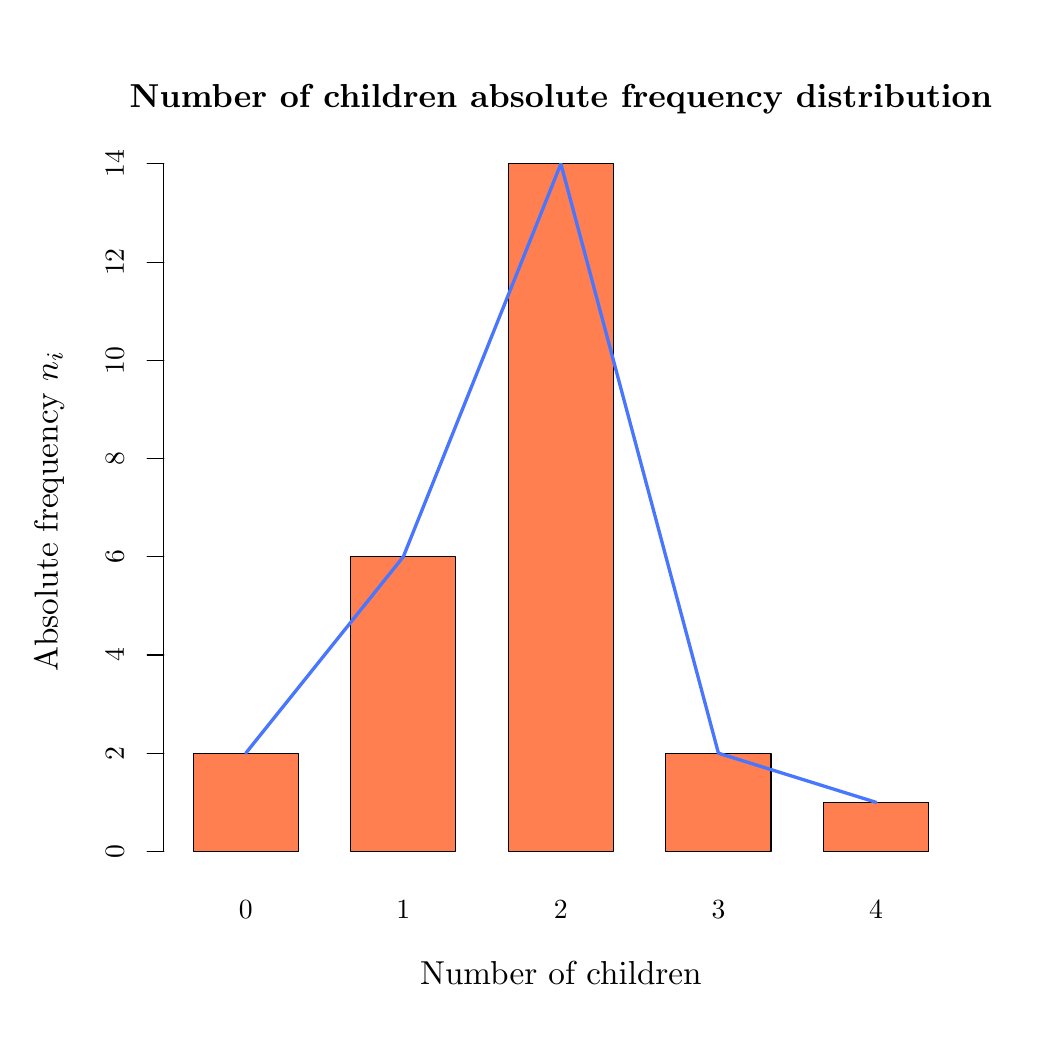
\begin{tikzpicture}[x=1pt,y=1pt]
\definecolor{fillColor}{RGB}{255,255,255}
\path[use as bounding box,fill=fillColor,fill opacity=0.00] (0,0) rectangle (361.35,361.35);
\begin{scope}
\path[clip] (  0.00,  0.00) rectangle (361.35,361.35);
\definecolor{drawColor}{RGB}{0,0,0}
\definecolor{fillColor}{RGB}{255,127,80}

\path[draw=drawColor,line width= 0.4pt,line join=round,line cap=round,fill=fillColor] ( 59.83, 63.68) rectangle ( 97.78, 99.18);

\path[draw=drawColor,line width= 0.4pt,line join=round,line cap=round,fill=fillColor] (116.76, 63.68) rectangle (154.72,170.17);

\path[draw=drawColor,line width= 0.4pt,line join=round,line cap=round,fill=fillColor] (173.70, 63.68) rectangle (211.65,312.15);

\path[draw=drawColor,line width= 0.4pt,line join=round,line cap=round,fill=fillColor] (230.63, 63.68) rectangle (268.59, 99.18);

\path[draw=drawColor,line width= 0.4pt,line join=round,line cap=round,fill=fillColor] (287.57, 63.68) rectangle (325.52, 81.43);
\end{scope}
\begin{scope}
\path[clip] (  0.00,  0.00) rectangle (361.35,361.35);
\definecolor{drawColor}{RGB}{0,0,0}

\node[text=drawColor,anchor=base,inner sep=0pt, outer sep=0pt, scale=  1.00] at ( 78.81, 39.60) {0};

\node[text=drawColor,anchor=base,inner sep=0pt, outer sep=0pt, scale=  1.00] at (135.74, 39.60) {1};

\node[text=drawColor,anchor=base,inner sep=0pt, outer sep=0pt, scale=  1.00] at (192.67, 39.60) {2};

\node[text=drawColor,anchor=base,inner sep=0pt, outer sep=0pt, scale=  1.00] at (249.61, 39.60) {3};

\node[text=drawColor,anchor=base,inner sep=0pt, outer sep=0pt, scale=  1.00] at (306.54, 39.60) {4};
\end{scope}
\begin{scope}
\path[clip] (  0.00,  0.00) rectangle (361.35,361.35);
\definecolor{drawColor}{RGB}{0,0,0}

\node[text=drawColor,anchor=base,inner sep=0pt, outer sep=0pt, scale=  1.20] at (192.68,332.61) {\bfseries Number of children absolute frequency distribution};

\node[text=drawColor,anchor=base,inner sep=0pt, outer sep=0pt, scale=  1.20] at (192.68, 15.60) {Number of children};

\node[text=drawColor,rotate= 90.00,anchor=base,inner sep=0pt, outer sep=0pt, scale=  1.20] at ( 10.80,186.67) {Absolute frequency $n_i$};
\end{scope}
\begin{scope}
\path[clip] (  0.00,  0.00) rectangle (361.35,361.35);
\definecolor{drawColor}{RGB}{0,0,0}

\path[draw=drawColor,line width= 0.4pt,line join=round,line cap=round] ( 49.20, 63.68) -- ( 49.20,312.15);

\path[draw=drawColor,line width= 0.4pt,line join=round,line cap=round] ( 49.20, 63.68) -- ( 43.20, 63.68);

\path[draw=drawColor,line width= 0.4pt,line join=round,line cap=round] ( 49.20, 99.18) -- ( 43.20, 99.18);

\path[draw=drawColor,line width= 0.4pt,line join=round,line cap=round] ( 49.20,134.67) -- ( 43.20,134.67);

\path[draw=drawColor,line width= 0.4pt,line join=round,line cap=round] ( 49.20,170.17) -- ( 43.20,170.17);

\path[draw=drawColor,line width= 0.4pt,line join=round,line cap=round] ( 49.20,205.66) -- ( 43.20,205.66);

\path[draw=drawColor,line width= 0.4pt,line join=round,line cap=round] ( 49.20,241.16) -- ( 43.20,241.16);

\path[draw=drawColor,line width= 0.4pt,line join=round,line cap=round] ( 49.20,276.65) -- ( 43.20,276.65);

\path[draw=drawColor,line width= 0.4pt,line join=round,line cap=round] ( 49.20,312.15) -- ( 43.20,312.15);

\node[text=drawColor,rotate= 90.00,anchor=base,inner sep=0pt, outer sep=0pt, scale=  1.00] at ( 34.80, 63.68) {0};

\node[text=drawColor,rotate= 90.00,anchor=base,inner sep=0pt, outer sep=0pt, scale=  1.00] at ( 34.80, 99.18) {2};

\node[text=drawColor,rotate= 90.00,anchor=base,inner sep=0pt, outer sep=0pt, scale=  1.00] at ( 34.80,134.67) {4};

\node[text=drawColor,rotate= 90.00,anchor=base,inner sep=0pt, outer sep=0pt, scale=  1.00] at ( 34.80,170.17) {6};

\node[text=drawColor,rotate= 90.00,anchor=base,inner sep=0pt, outer sep=0pt, scale=  1.00] at ( 34.80,205.66) {8};

\node[text=drawColor,rotate= 90.00,anchor=base,inner sep=0pt, outer sep=0pt, scale=  1.00] at ( 34.80,241.16) {10};

\node[text=drawColor,rotate= 90.00,anchor=base,inner sep=0pt, outer sep=0pt, scale=  1.00] at ( 34.80,276.65) {12};

\node[text=drawColor,rotate= 90.00,anchor=base,inner sep=0pt, outer sep=0pt, scale=  1.00] at ( 34.80,312.15) {14};
\end{scope}
\begin{scope}
\path[clip] ( 49.20, 61.20) rectangle (336.15,312.15);
\definecolor{drawColor}{RGB}{72,118,255}

\path[draw=drawColor,line width= 1.2pt,line join=round,line cap=round] ( 78.81, 99.18) --
	(135.74,170.17) --
	(192.67,312.15) --
	(249.61, 99.18) --
	(306.54, 81.43);
\end{scope}
\end{tikzpicture}
} 
\end{center}
\end{frame}


%---------------------------------------------------------------------slide----
\begin{frame}
\frametitle{Cumulative absolute frequency bar chart}
\framesubtitle{Non-grouped data}
\begin{center}
\scalebox{0.6}{\input{img/descriptive/cum_abs_freq_bar_chart}} 
\end{center}
\end{frame}


%---------------------------------------------------------------------slide----
\begin{frame}
\frametitle{Cumulative absolute frequency line chart or polygon}
\framesubtitle{Non-grouped data}
\begin{center}
\scalebox{0.6}{% Created by tikzDevice version 0.8.1 on 2015-11-09 17:45:22
% !TEX encoding = UTF-8 Unicode
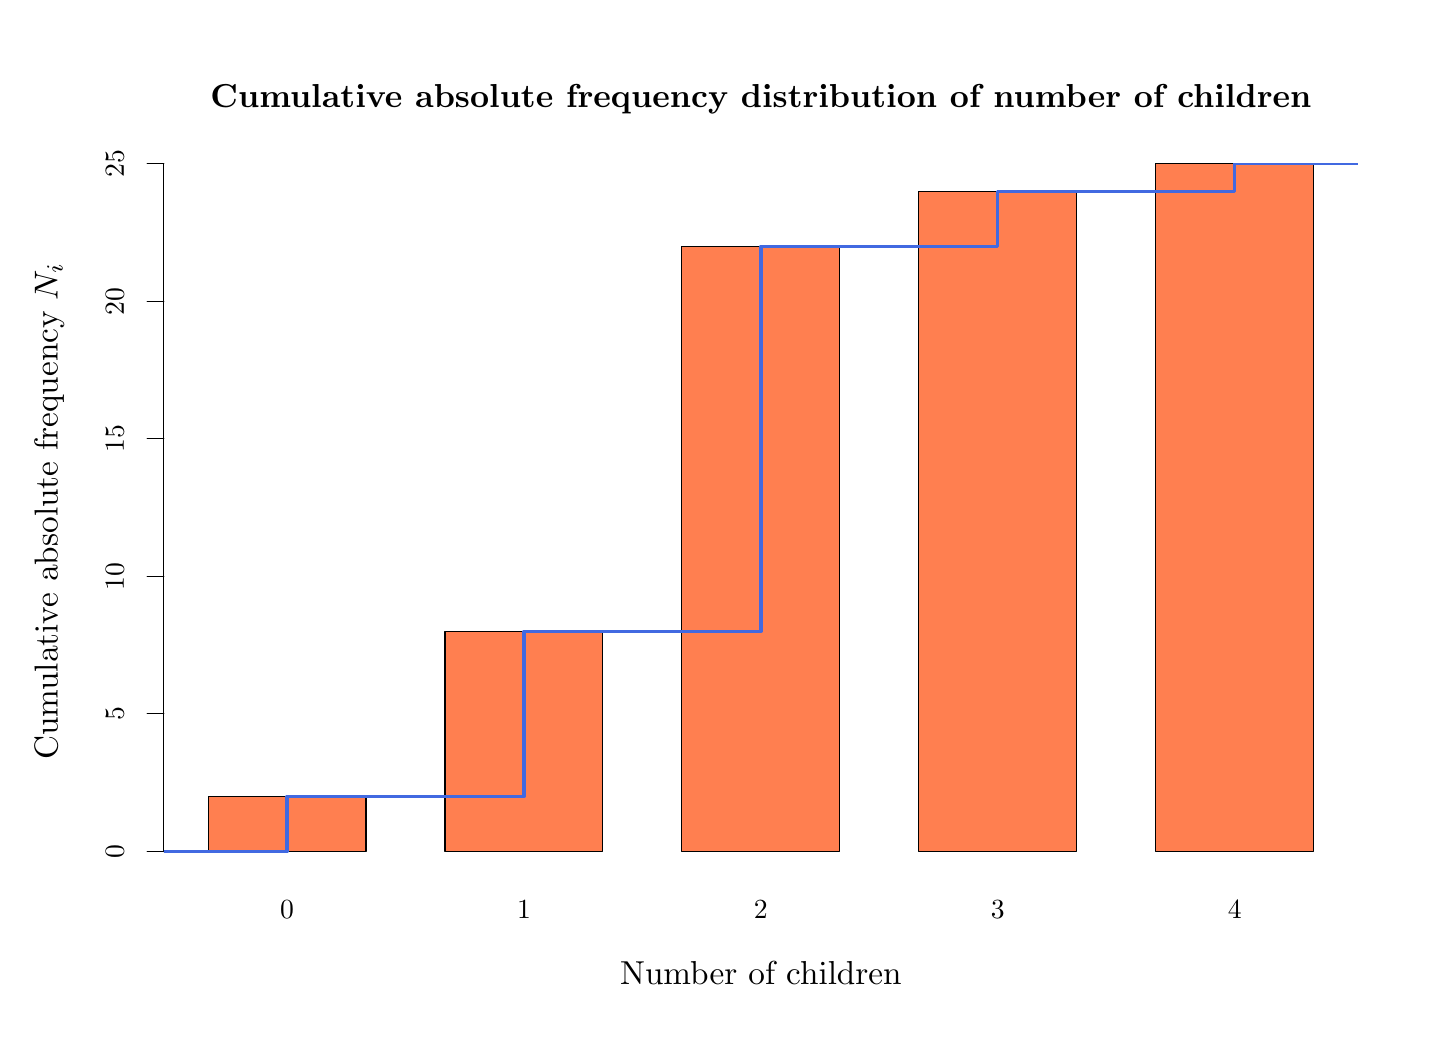
\begin{tikzpicture}[x=1pt,y=1pt]
\definecolor{fillColor}{RGB}{255,255,255}
\path[use as bounding box,fill=fillColor,fill opacity=0.00] (0,0) rectangle (505.89,361.35);
\begin{scope}
\path[clip] (  0.00,  0.00) rectangle (505.89,361.35);
\definecolor{drawColor}{RGB}{0,0,0}
\definecolor{fillColor}{RGB}{255,127,80}

\path[draw=drawColor,line width= 0.4pt,line join=round,line cap=round,fill=fillColor] ( 65.18, 63.68) rectangle (122.26, 83.56);

\path[draw=drawColor,line width= 0.4pt,line join=round,line cap=round,fill=fillColor] (150.79, 63.68) rectangle (207.87,143.19);

\path[draw=drawColor,line width= 0.4pt,line join=round,line cap=round,fill=fillColor] (236.41, 63.68) rectangle (293.48,282.33);

\path[draw=drawColor,line width= 0.4pt,line join=round,line cap=round,fill=fillColor] (322.02, 63.68) rectangle (379.10,302.21);

\path[draw=drawColor,line width= 0.4pt,line join=round,line cap=round,fill=fillColor] (407.63, 63.68) rectangle (464.71,312.15);
\end{scope}
\begin{scope}
\path[clip] (  0.00,  0.00) rectangle (505.89,361.35);
\definecolor{drawColor}{RGB}{0,0,0}

\node[text=drawColor,anchor=base,inner sep=0pt, outer sep=0pt, scale=  1.00] at ( 93.72, 39.60) {0};

\node[text=drawColor,anchor=base,inner sep=0pt, outer sep=0pt, scale=  1.00] at (179.33, 39.60) {1};

\node[text=drawColor,anchor=base,inner sep=0pt, outer sep=0pt, scale=  1.00] at (264.94, 39.60) {2};

\node[text=drawColor,anchor=base,inner sep=0pt, outer sep=0pt, scale=  1.00] at (350.56, 39.60) {3};

\node[text=drawColor,anchor=base,inner sep=0pt, outer sep=0pt, scale=  1.00] at (436.17, 39.60) {4};
\end{scope}
\begin{scope}
\path[clip] (  0.00,  0.00) rectangle (505.89,361.35);
\definecolor{drawColor}{RGB}{0,0,0}

\node[text=drawColor,anchor=base,inner sep=0pt, outer sep=0pt, scale=  1.20] at (264.94,332.61) {\bfseries Cumulative absolute frequency distribution of number of children};

\node[text=drawColor,anchor=base,inner sep=0pt, outer sep=0pt, scale=  1.20] at (264.94, 15.60) {Number of children};

\node[text=drawColor,rotate= 90.00,anchor=base,inner sep=0pt, outer sep=0pt, scale=  1.20] at ( 10.80,186.67) {Cumulative absolute frequency $N_i$};
\end{scope}
\begin{scope}
\path[clip] (  0.00,  0.00) rectangle (505.89,361.35);
\definecolor{drawColor}{RGB}{0,0,0}

\path[draw=drawColor,line width= 0.4pt,line join=round,line cap=round] ( 49.20, 63.68) -- ( 49.20,312.15);

\path[draw=drawColor,line width= 0.4pt,line join=round,line cap=round] ( 49.20, 63.68) -- ( 43.20, 63.68);

\path[draw=drawColor,line width= 0.4pt,line join=round,line cap=round] ( 49.20,113.38) -- ( 43.20,113.38);

\path[draw=drawColor,line width= 0.4pt,line join=round,line cap=round] ( 49.20,163.07) -- ( 43.20,163.07);

\path[draw=drawColor,line width= 0.4pt,line join=round,line cap=round] ( 49.20,212.76) -- ( 43.20,212.76);

\path[draw=drawColor,line width= 0.4pt,line join=round,line cap=round] ( 49.20,262.46) -- ( 43.20,262.46);

\path[draw=drawColor,line width= 0.4pt,line join=round,line cap=round] ( 49.20,312.15) -- ( 43.20,312.15);

\node[text=drawColor,rotate= 90.00,anchor=base,inner sep=0pt, outer sep=0pt, scale=  1.00] at ( 34.80, 63.68) {0};

\node[text=drawColor,rotate= 90.00,anchor=base,inner sep=0pt, outer sep=0pt, scale=  1.00] at ( 34.80,113.38) {5};

\node[text=drawColor,rotate= 90.00,anchor=base,inner sep=0pt, outer sep=0pt, scale=  1.00] at ( 34.80,163.07) {10};

\node[text=drawColor,rotate= 90.00,anchor=base,inner sep=0pt, outer sep=0pt, scale=  1.00] at ( 34.80,212.76) {15};

\node[text=drawColor,rotate= 90.00,anchor=base,inner sep=0pt, outer sep=0pt, scale=  1.00] at ( 34.80,262.46) {20};

\node[text=drawColor,rotate= 90.00,anchor=base,inner sep=0pt, outer sep=0pt, scale=  1.00] at ( 34.80,312.15) {25};
\end{scope}
\begin{scope}
\path[clip] ( 49.20, 61.20) rectangle (480.69,312.15);
\definecolor{drawColor}{RGB}{65,105,225}

\path[draw=drawColor,line width= 1.2pt,line join=round,line cap=round] ( 36.64, 63.68) --
	( 93.72, 63.68) --
	( 93.72, 83.56) --
	(179.33, 83.56) --
	(179.33,143.19) --
	(264.94,143.19) --
	(264.94,282.33) --
	(350.56,282.33) --
	(350.56,302.21) --
	(436.17,302.21) --
	(436.17,312.15) --
	(505.89,312.15);
\end{scope}
\end{tikzpicture}
} 
\end{center} 
\end{frame}


%---------------------------------------------------------------------slide----
\begin{frame}
\frametitle{Histogram}
A \structure{histogram} is similar to a bar chart but for grouped data.  

Usually the classes or grouping intervals are represented on the $x$-axis, and the frequencies on the $y$-axis. 
For each class, a bar is draw to the height of its frequency.
Contrary to bar charts, the width of bars coincides with the width of classes, and there are no space between two
consecutive bars.

Depending on the type of frequency represented in the $y$-axis we get different types of histograms.
 
Sometimes a polygon, known as \structure{\textbf{frequency polygon}}, is plotted joining the top of every bar.
\end{frame}


%---------------------------------------------------------------------slide----
\begin{frame}
\frametitle{Absolute frequency histogram}
\framesubtitle{Grouped data}
\begin{center}
\scalebox{0.6}{% Created by tikzDevice version 0.8.1 on 2015-11-09 19:19:11
% !TEX encoding = UTF-8 Unicode
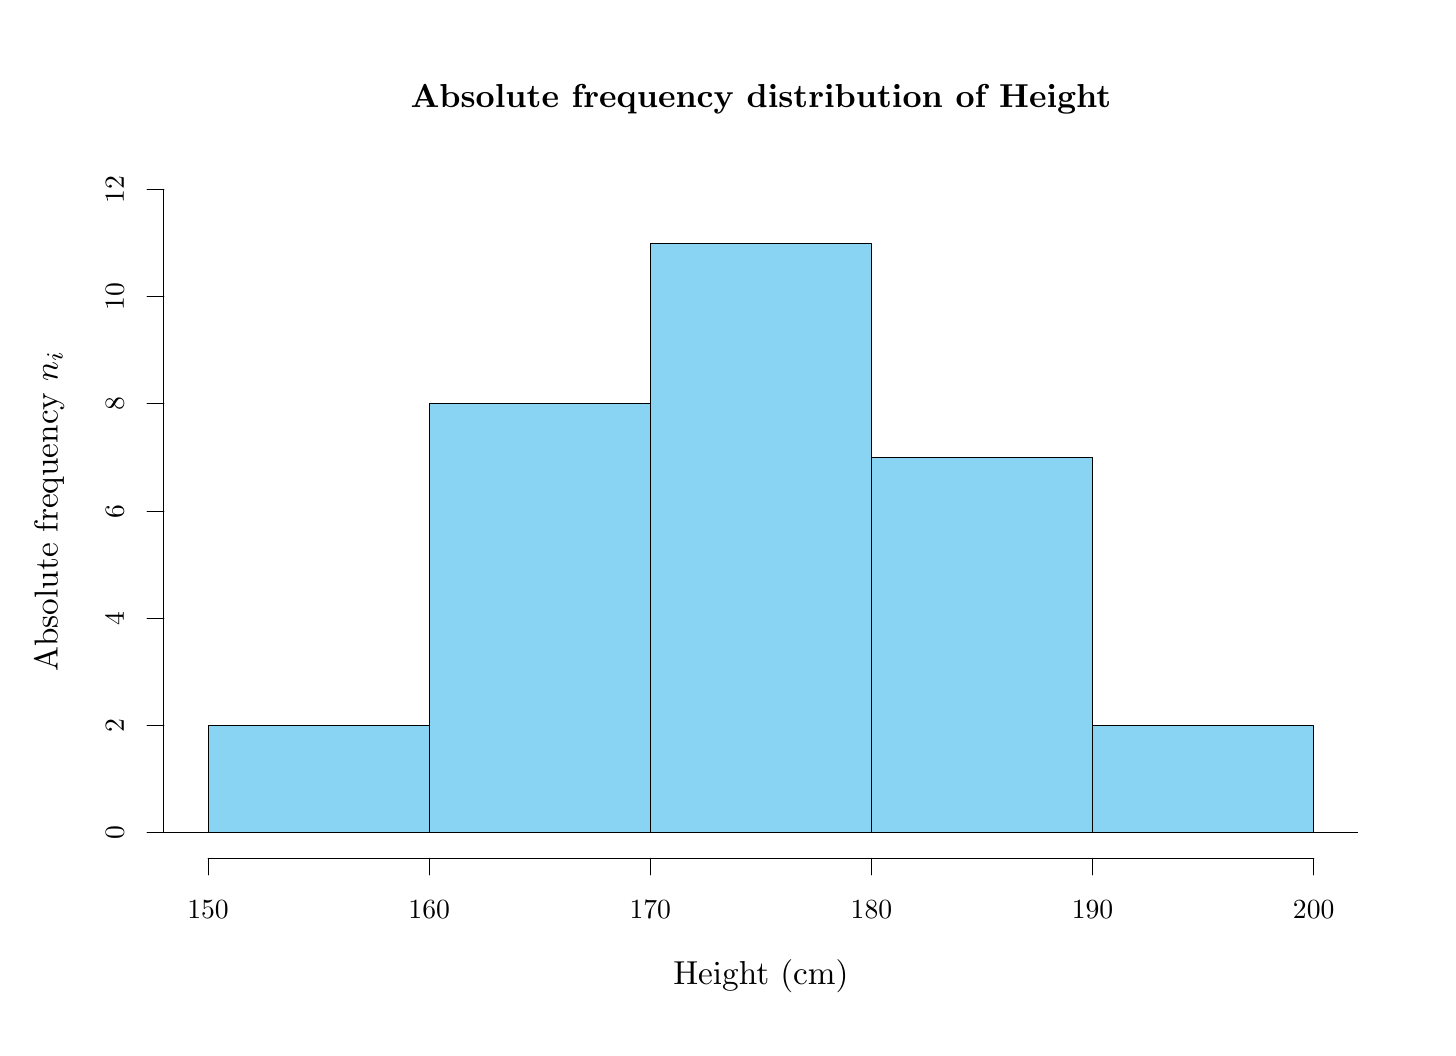
\begin{tikzpicture}[x=1pt,y=1pt]
\definecolor{fillColor}{RGB}{255,255,255}
\path[use as bounding box,fill=fillColor,fill opacity=0.00] (0,0) rectangle (505.89,361.35);
\begin{scope}
\path[clip] (  0.00,  0.00) rectangle (505.89,361.35);
\definecolor{drawColor}{RGB}{0,0,0}

\node[text=drawColor,anchor=base,inner sep=0pt, outer sep=0pt, scale=  1.20] at (264.95,332.61) {\bfseries Absolute frequency distribution of Height};

\node[text=drawColor,anchor=base,inner sep=0pt, outer sep=0pt, scale=  1.20] at (264.95, 15.60) {Height (cm)};

\node[text=drawColor,rotate= 90.00,anchor=base,inner sep=0pt, outer sep=0pt, scale=  1.20] at ( 10.80,186.67) {Absolute frequency $n_i$};
\end{scope}
\begin{scope}
\path[clip] (  0.00,  0.00) rectangle (505.89,361.35);
\definecolor{drawColor}{RGB}{0,0,0}

\path[draw=drawColor,line width= 0.4pt,line join=round,line cap=round] ( 65.18, 61.20) -- (464.71, 61.20);

\path[draw=drawColor,line width= 0.4pt,line join=round,line cap=round] ( 65.18, 61.20) -- ( 65.18, 55.20);

\path[draw=drawColor,line width= 0.4pt,line join=round,line cap=round] (145.09, 61.20) -- (145.09, 55.20);

\path[draw=drawColor,line width= 0.4pt,line join=round,line cap=round] (224.99, 61.20) -- (224.99, 55.20);

\path[draw=drawColor,line width= 0.4pt,line join=round,line cap=round] (304.90, 61.20) -- (304.90, 55.20);

\path[draw=drawColor,line width= 0.4pt,line join=round,line cap=round] (384.80, 61.20) -- (384.80, 55.20);

\path[draw=drawColor,line width= 0.4pt,line join=round,line cap=round] (464.71, 61.20) -- (464.71, 55.20);

\node[text=drawColor,anchor=base,inner sep=0pt, outer sep=0pt, scale=  1.00] at ( 65.18, 39.60) {150};

\node[text=drawColor,anchor=base,inner sep=0pt, outer sep=0pt, scale=  1.00] at (145.09, 39.60) {160};

\node[text=drawColor,anchor=base,inner sep=0pt, outer sep=0pt, scale=  1.00] at (224.99, 39.60) {170};

\node[text=drawColor,anchor=base,inner sep=0pt, outer sep=0pt, scale=  1.00] at (304.90, 39.60) {180};

\node[text=drawColor,anchor=base,inner sep=0pt, outer sep=0pt, scale=  1.00] at (384.80, 39.60) {190};

\node[text=drawColor,anchor=base,inner sep=0pt, outer sep=0pt, scale=  1.00] at (464.71, 39.60) {200};

\path[draw=drawColor,line width= 0.4pt,line join=round,line cap=round] ( 49.20, 70.49) -- ( 49.20,302.86);

\path[draw=drawColor,line width= 0.4pt,line join=round,line cap=round] ( 49.20, 70.49) -- ( 43.20, 70.49);

\path[draw=drawColor,line width= 0.4pt,line join=round,line cap=round] ( 49.20,109.22) -- ( 43.20,109.22);

\path[draw=drawColor,line width= 0.4pt,line join=round,line cap=round] ( 49.20,147.95) -- ( 43.20,147.95);

\path[draw=drawColor,line width= 0.4pt,line join=round,line cap=round] ( 49.20,186.67) -- ( 43.20,186.67);

\path[draw=drawColor,line width= 0.4pt,line join=round,line cap=round] ( 49.20,225.40) -- ( 43.20,225.40);

\path[draw=drawColor,line width= 0.4pt,line join=round,line cap=round] ( 49.20,264.13) -- ( 43.20,264.13);

\path[draw=drawColor,line width= 0.4pt,line join=round,line cap=round] ( 49.20,302.86) -- ( 43.20,302.86);

\node[text=drawColor,rotate= 90.00,anchor=base,inner sep=0pt, outer sep=0pt, scale=  1.00] at ( 34.80, 70.49) {0};

\node[text=drawColor,rotate= 90.00,anchor=base,inner sep=0pt, outer sep=0pt, scale=  1.00] at ( 34.80,109.22) {2};

\node[text=drawColor,rotate= 90.00,anchor=base,inner sep=0pt, outer sep=0pt, scale=  1.00] at ( 34.80,147.95) {4};

\node[text=drawColor,rotate= 90.00,anchor=base,inner sep=0pt, outer sep=0pt, scale=  1.00] at ( 34.80,186.67) {6};

\node[text=drawColor,rotate= 90.00,anchor=base,inner sep=0pt, outer sep=0pt, scale=  1.00] at ( 34.80,225.40) {8};

\node[text=drawColor,rotate= 90.00,anchor=base,inner sep=0pt, outer sep=0pt, scale=  1.00] at ( 34.80,264.13) {10};

\node[text=drawColor,rotate= 90.00,anchor=base,inner sep=0pt, outer sep=0pt, scale=  1.00] at ( 34.80,302.86) {12};
\end{scope}
\begin{scope}
\path[clip] ( 49.20, 61.20) rectangle (480.69,312.15);
\definecolor{drawColor}{RGB}{0,0,0}
\definecolor{fillColor}{RGB}{137,211,243}

\path[draw=drawColor,line width= 0.4pt,line join=round,line cap=round,fill=fillColor] ( 65.18, 70.49) rectangle (145.09,109.22);

\path[draw=drawColor,line width= 0.4pt,line join=round,line cap=round,fill=fillColor] (145.09, 70.49) rectangle (224.99,225.40);

\path[draw=drawColor,line width= 0.4pt,line join=round,line cap=round,fill=fillColor] (224.99, 70.49) rectangle (304.90,283.49);

\path[draw=drawColor,line width= 0.4pt,line join=round,line cap=round,fill=fillColor] (304.90, 70.49) rectangle (384.80,206.04);

\path[draw=drawColor,line width= 0.4pt,line join=round,line cap=round,fill=fillColor] (384.80, 70.49) rectangle (464.71,109.22);
\definecolor{drawColor}{RGB}{238,50,36}


\definecolor{drawColor}{RGB}{0,0,0}

\path[draw=drawColor,line width= 0.4pt,line join=round,line cap=round] ( 49.20, 70.49) -- (480.69, 70.49);
\end{scope}
\end{tikzpicture}
}
\end{center} 
\end{frame}


%---------------------------------------------------------------------slide----
\begin{frame}
\frametitle{Absolute frequency histogram}
\framesubtitle{Grouped data}
\begin{center}
\scalebox{0.6}{\input{img/descriptive/abs_freq_histogram_polygon}} 
\end{center} 
\end{frame}


%---------------------------------------------------------------------slide----
\begin{frame}
\frametitle{Cumulative absolute frequency histogram}
\framesubtitle{Grouped data}
\begin{center}
\scalebox{0.6}{\input{img/descriptive/cum_abs_freq_histogram}}
\end{center} 
\end{frame}


%---------------------------------------------------------------------slide----
\begin{frame}
\frametitle{Cumulative absolute frequency line chart or ogive}
\framesubtitle{Grouped data}
\begin{center}
\scalebox{0.6}{\input{img/descriptive/cum_abs_freq_histogram_polygon}} 
\end{center} 
\end{frame}


%---------------------------------------------------------------------slide----
\begin{frame}
\frametitle{Cumulative relative frequency histogram}
\framesubtitle{Grouped data}
\begin{center}
\scalebox{0.6}{\input{img/descriptive/cum_rel_freq_histogram}}
\end{center} 
\end{frame}


%---------------------------------------------------------------------slide----
\begin{frame}
\frametitle{Cumulative relative frequency line chart or ogive}
\framesubtitle{Grouped data}
\begin{center}
\scalebox{0.6}{\input{img/descriptive/cum_rel_freq_histogram_polygon}} 
\end{center} 
\end{frame}
 

%---------------------------------------------------------------------slide----
\begin{frame}
\frametitle{Pie chart}
A \structure{pie chart} consists in a circle divided in slices, one for every value or category of the variable. 
Each slice is called \structure{sector} and its angle or area is proportional to the frequency of the corresponding
value or category. 

Pie charts can represent absolute or relative frequencies, but not cumulative frequencies, and are used with nominal
qualitative variables.
For ordinal qualitative or quantitative variables is better to use bar charts or histograms, cause it's easy to perceive
differences in one dimension (lenght of bars) than in two dimensions (areas of sectors).
\end{frame}


%---------------------------------------------------------------------slide----
\begin{frame}
\frametitle{Pie chart}
\framesubtitle{Nominal variables}
\begin{center}
\scalebox{0.6}{% Created by tikzDevice version 0.8.1 on 2015-11-09 20:32:18
% !TEX encoding = UTF-8 Unicode
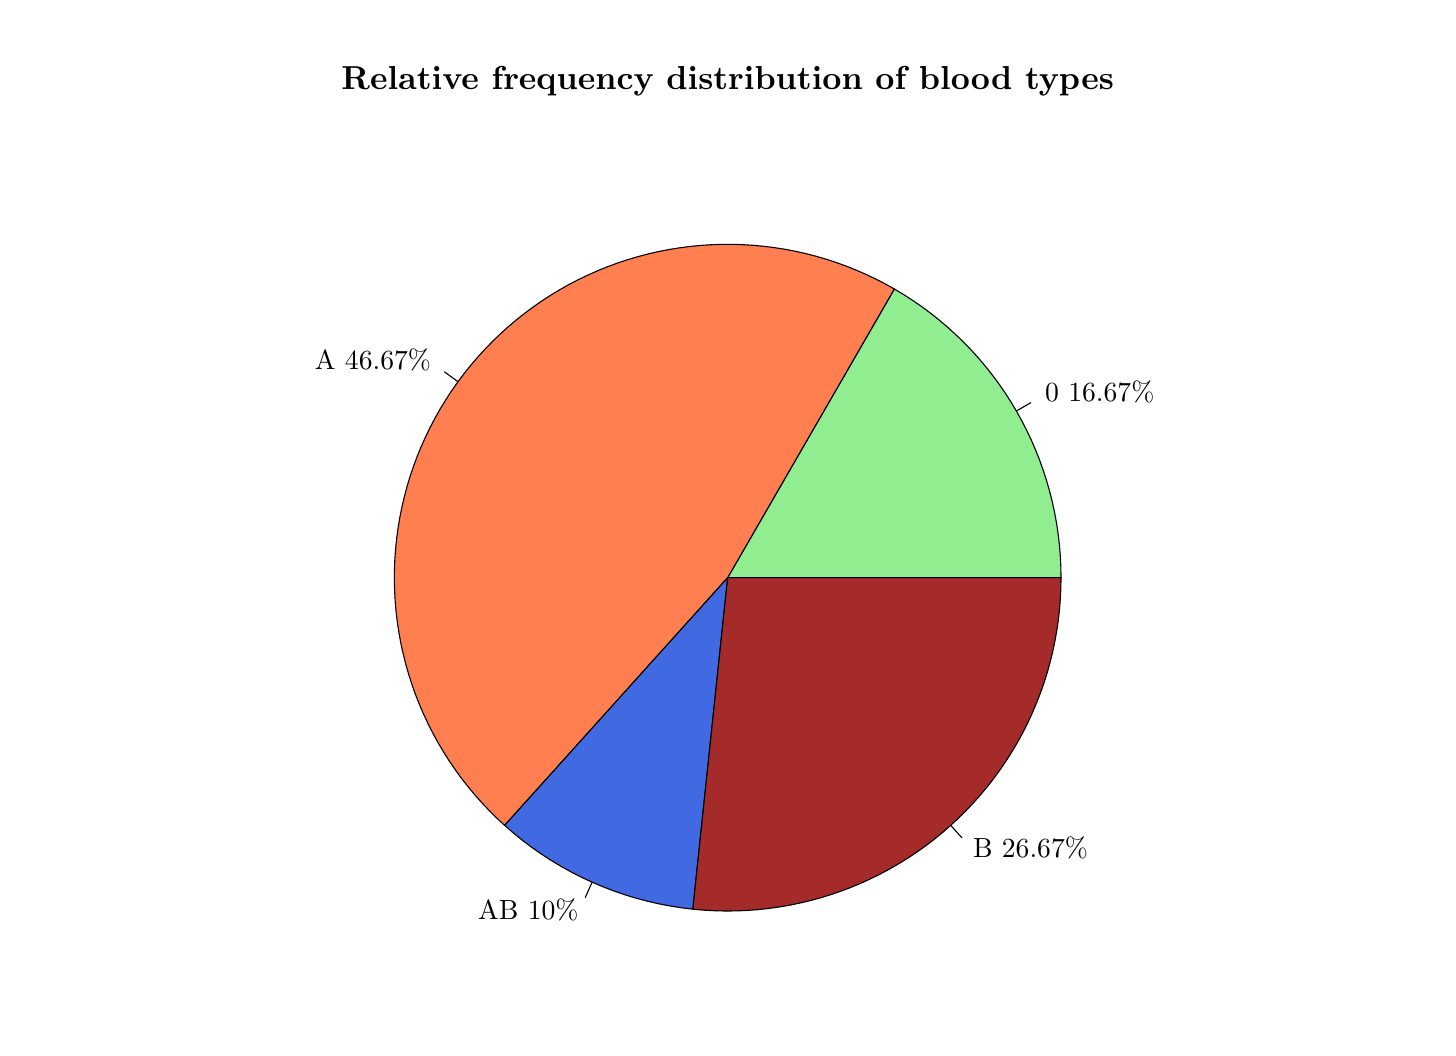
\begin{tikzpicture}[x=1pt,y=1pt]
\definecolor{fillColor}{RGB}{255,255,255}
\path[use as bounding box,fill=fillColor,fill opacity=0.00] (0,0) rectangle (505.89,361.35);
\begin{scope}
\path[clip] (  0.00,  0.00) rectangle (505.89,325.21);
\definecolor{drawColor}{RGB}{0,0,0}
\definecolor{fillColor}{RGB}{144,238,144}

\path[draw=drawColor,line width= 0.4pt,line join=round,line cap=round,fill=fillColor] (373.40,162.61) --
	(373.33,166.55) --
	(373.14,170.49) --
	(372.82,174.41) --
	(372.36,178.33) --
	(371.79,182.23) --
	(371.08,186.11) --
	(370.25,189.96) --
	(369.29,193.78) --
	(368.21,197.57) --
	(367.00,201.32) --
	(365.67,205.04) --
	(364.23,208.70) --
	(362.66,212.32) --
	(360.97,215.88) --
	(359.17,219.39) --
	(357.26,222.83) --
	(355.23,226.21) --
	(353.10,229.53) --
	(350.85,232.77) --
	(348.50,235.93) --
	(346.05,239.02) --
	(343.50,242.03) --
	(340.86,244.95) --
	(338.12,247.78) --
	(335.28,250.52) --
	(332.36,253.17) --
	(329.36,255.72) --
	(326.27,258.17) --
	(323.10,260.51) --
	(319.86,262.76) --
	(316.55,264.89) --
	(313.17,266.92) --
	(252.94,162.61) --
	cycle;

\path[draw=drawColor,line width= 0.4pt,line join=round,line cap=round] (357.26,222.83) --
	(362.47,225.84);
\end{scope}
\begin{scope}
\path[clip] (  0.00,  0.00) rectangle (505.89,361.35);
\definecolor{drawColor}{RGB}{0,0,0}

\node[text=drawColor,anchor=base west,inner sep=0pt, outer sep=0pt, scale=  1.00] at (367.69,226.36) {0 16.67\%};
\end{scope}
\begin{scope}
\path[clip] (  0.00,  0.00) rectangle (505.89,325.21);
\definecolor{drawColor}{RGB}{0,0,0}
\definecolor{fillColor}{RGB}{255,127,80}

\path[draw=drawColor,line width= 0.4pt,line join=round,line cap=round,fill=fillColor] (313.17,266.92) --
	(309.82,268.79) --
	(306.40,270.54) --
	(302.94,272.19) --
	(299.42,273.73) --
	(295.85,275.16) --
	(292.25,276.47) --
	(288.60,277.66) --
	(284.91,278.74) --
	(281.20,279.70) --
	(277.45,280.54) --
	(273.68,281.26) --
	(269.89,281.86) --
	(266.08,282.34) --
	(262.26,282.70) --
	(258.43,282.93) --
	(254.59,283.05) --
	(250.75,283.04) --
	(246.91,282.91) --
	(243.08,282.65) --
	(239.26,282.28) --
	(235.46,281.78) --
	(231.67,281.16) --
	(227.90,280.43) --
	(224.16,279.57) --
	(220.45,278.59) --
	(216.77,277.50) --
	(213.13,276.29) --
	(209.52,274.96) --
	(205.97,273.52) --
	(202.46,271.96) --
	(199.00,270.30) --
	(195.59,268.53) --
	(192.25,266.64) --
	(188.96,264.66) --
	(185.74,262.57) --
	(182.59,260.37) --
	(179.51,258.08) --
	(176.51,255.69) --
	(173.58,253.21) --
	(170.73,250.64) --
	(167.97,247.97) --
	(165.29,245.22) --
	(162.70,242.39) --
	(160.21,239.47) --
	(157.80,236.48) --
	(155.50,233.41) --
	(153.29,230.27) --
	(151.19,227.06) --
	(149.18,223.78) --
	(147.29,220.44) --
	(145.50,217.05) --
	(143.82,213.59) --
	(142.25,210.09) --
	(140.79,206.54) --
	(139.45,202.94) --
	(138.22,199.31) --
	(137.11,195.63) --
	(136.12,191.92) --
	(135.24,188.19) --
	(134.49,184.42) --
	(133.85,180.64) --
	(133.34,176.83) --
	(132.95,173.01) --
	(132.67,169.19) --
	(132.53,165.35) --
	(132.50,161.51) --
	(132.60,157.67) --
	(132.81,153.84) --
	(133.15,150.02) --
	(133.62,146.21) --
	(134.20,142.41) --
	(134.90,138.64) --
	(135.73,134.89) --
	(136.67,131.17) --
	(137.73,127.48) --
	(138.91,123.83) --
	(140.20,120.21) --
	(141.61,116.64) --
	(143.13,113.12) --
	(144.77,109.64) --
	(146.51,106.22) --
	(148.36,102.86) --
	(150.32, 99.56) --
	(152.38, 96.32) --
	(154.54, 93.15) --
	(156.80, 90.05) --
	(159.17, 87.02) --
	(161.62, 84.07) --
	(164.17, 81.20) --
	(166.81, 78.41) --
	(169.54, 75.71) --
	(172.35, 73.10) --
	(252.94,162.61) --
	cycle;

\path[draw=drawColor,line width= 0.4pt,line join=round,line cap=round] (155.50,233.41) --
	(150.63,236.95);
\end{scope}
\begin{scope}
\path[clip] (  0.00,  0.00) rectangle (505.89,361.35);
\definecolor{drawColor}{RGB}{0,0,0}

\node[text=drawColor,anchor=base east,inner sep=0pt, outer sep=0pt, scale=  1.00] at (145.75,237.99) {A 46.67\%};
\end{scope}
\begin{scope}
\path[clip] (  0.00,  0.00) rectangle (505.89,325.21);
\definecolor{drawColor}{RGB}{0,0,0}
\definecolor{fillColor}{RGB}{65,105,225}

\path[draw=drawColor,line width= 0.4pt,line join=round,line cap=round,fill=fillColor] (172.35, 73.10) --
	(175.52, 70.34) --
	(178.79, 67.69) --
	(182.15, 65.16) --
	(185.59, 62.75) --
	(189.12, 60.46) --
	(192.72, 58.29) --
	(196.40, 56.26) --
	(200.14, 54.35) --
	(203.95, 52.57) --
	(207.82, 50.93) --
	(211.75, 49.42) --
	(215.72, 48.05) --
	(219.74, 46.82) --
	(223.81, 45.74) --
	(227.90, 44.79) --
	(232.03, 43.99) --
	(236.18, 43.33) --
	(240.35, 42.82) --
	(252.94,162.61) --
	cycle;

\path[draw=drawColor,line width= 0.4pt,line join=round,line cap=round] (203.95, 52.57) --
	(201.50, 47.07);
\end{scope}
\begin{scope}
\path[clip] (  0.00,  0.00) rectangle (505.89,361.35);
\definecolor{drawColor}{RGB}{0,0,0}

\node[text=drawColor,anchor=base east,inner sep=0pt, outer sep=0pt, scale=  1.00] at (199.05, 39.07) {AB 10\%};
\end{scope}
\begin{scope}
\path[clip] (  0.00,  0.00) rectangle (505.89,325.21);
\definecolor{drawColor}{RGB}{0,0,0}
\definecolor{fillColor}{RGB}{165,42,42}

\path[draw=drawColor,line width= 0.4pt,line join=round,line cap=round,fill=fillColor] (240.35, 42.82) --
	(244.22, 42.47) --
	(248.09, 42.26) --
	(251.97, 42.16) --
	(255.86, 42.19) --
	(259.73, 42.35) --
	(263.60, 42.63) --
	(267.46, 43.04) --
	(271.31, 43.57) --
	(275.13, 44.22) --
	(278.94, 45.00) --
	(282.71, 45.89) --
	(286.46, 46.91) --
	(290.17, 48.05) --
	(293.84, 49.31) --
	(297.47, 50.69) --
	(301.05, 52.18) --
	(304.58, 53.79) --
	(308.06, 55.51) --
	(311.48, 57.34) --
	(314.84, 59.28) --
	(318.14, 61.33) --
	(321.37, 63.48) --
	(324.53, 65.73) --
	(327.61, 68.09) --
	(330.62, 70.55) --
	(333.54, 73.10) --
	(336.38, 75.74) --
	(339.14, 78.47) --
	(341.80, 81.29) --
	(344.38, 84.20) --
	(346.86, 87.18) --
	(349.24, 90.25) --
	(351.52, 93.39) --
	(353.70, 96.60) --
	(355.77, 99.88) --
	(357.74,103.22) --
	(359.60,106.63) --
	(361.35,110.10) --
	(362.98,113.62) --
	(364.50,117.19) --
	(365.91,120.80) --
	(367.20,124.46) --
	(368.37,128.17) --
	(369.42,131.90) --
	(370.34,135.67) --
	(371.15,139.47) --
	(371.84,143.29) --
	(372.40,147.13) --
	(372.83,150.98) --
	(373.14,154.85) --
	(373.33,158.73) --
	(373.40,162.61) --
	(252.94,162.61) --
	cycle;

\path[draw=drawColor,line width= 0.4pt,line join=round,line cap=round] (333.54, 73.10) --
	(337.57, 68.62);
\end{scope}
\begin{scope}
\path[clip] (  0.00,  0.00) rectangle (505.89,361.35);
\definecolor{drawColor}{RGB}{0,0,0}

\node[text=drawColor,anchor=base west,inner sep=0pt, outer sep=0pt, scale=  1.00] at (341.60, 61.65) {B 26.67\%};

\node[text=drawColor,anchor=base,inner sep=0pt, outer sep=0pt, scale=  1.20] at (252.94,339.14) {\bfseries Relative frequency distribution of blood types};
\end{scope}
\end{tikzpicture}
}
\end{center}
\end{frame}


% ---------------------------------------------------------------------slide----
\begin{frame}
\frametitle{Outliers}
One of the main problems in samples are \structure{\textbf{outliers}}, that are values very different from the rest of
values of the sample.
\begin{center}
\includegraphics[scale=0.5]{img/descriptive/outlier.png}
\end{center}

It's important to find out outliers before doing any analysis, cause \alert{\emph{outliers usually distort the
results}}.

They always appears in the ends of the distribution, and can be find out easily with a box and whiskers chart (as 
be showed later).
\end{frame}


%---------------------------------------------------------------------slide----
\begin{frame}
\frametitle{Outliers management}
With big samples outliers have less importance and can be left in the sample.

With small samples we have several options:

\begin{itemize}
\item Remove the outlier if it's an error. 
\item Replace the outlier by the lower or higher value in the distribution that is not an outlier if it's not an error
and the outlier doesn't fit the theoretical distribution. 
\item Leave the outlier if it's not an error, and change the theoretical model to fit it to outliers.  
\end{itemize}
\end{frame}
 


\subsection{Sample statistics}

%---------------------------------------------------------------------slide----
\begin{frame}
\frametitle{Sample statistics}
The frequency table and charts summarize and give an overview of the distribution of values of the studied variable in
the sample, but it's difficult to describe some aspects of the distribution from it, as for example, which are the most
representative values of the distribution, how is the spread of data, which data could be considered outliers, how is
the symmetry of the distribution. 

To describe those aspects of the sample distribution more specific numerical measures, called
\structure{\textbf{sample statistics}}, are used.

According to the aspect of the distribution that they study, there are different types of statistics:
\begin{description}
\item[Measures of locations:] They measure the values where data are concentrated or that divide the distribution into
equal parts. 
\item[Measures of dispersion:] They measure the spread of data.
\item[Measures of shape:] They measure the symmetry and kurtosis of the distribution.  
\end{description}
\end{frame}


\subsection{Location statistics}

%---------------------------------------------------------------------slide----
\begin{frame}
\frametitle{Location statistics}
There are two groups: 

\begin{description}
\item [Central location measures:] They measure the values where data are concentrated, and that usually are in the
centre of the distribution. 
These values are the values that best represents the sample data. 
The most important are:
\begin{itemize}
\item Arithmetic mean
\item Median
\item Mode
\end{itemize}
\item [Non-central location measures:] They divide the sample data into equals parts. 
The most important are:
\begin{itemize}
\item Quartiles.
\item Deciles.
\item Percentiles. 
\end{itemize}
\end{description}
\end{frame}


%---------------------------------------------------------------------slide----
\begin{frame}
\frametitle{Arithmetic mean}
\begin{definition}[Sample arithmetic mean $\bar{x}$]
The \emph{sample arithmetic mean} of a variable $X$ is the sum of observed values in the sample divided by the sample
size
\[
\bar{x} = \frac{\sum x_i}{n}
\]
\end{definition}
From the frequency table can be calculated with the formula
\[
\bar{x} = \frac{\sum x_in_i}{n} = \sum x_i f_i
\]

In most cases the arithmetic mean is the value that best represent the observed values in the sample. 
\begin{center}
\alert{\emph{Watch out! It can not be calculated with qualitative variables.}}
\end{center}
\end{frame}


%---------------------------------------------------------------------slide----
\begin{frame}
\frametitle{Arithmetic mean calculation}
\framesubtitle{Example with non-grouped data}
Using the data of the sample with the number of children of families, the arithmetic mean is 
\begin{align*}
\bar{x} &= \frac{1+2+4+2+2+2+3+2+1+1+0+2+2}{25}+\\
&+\frac{0+2+2+1+2+2+3+1+2+2+1+2}{25} = \frac{44}{25} = 1.76 \mbox{ hijos}.
\end{align*}
or using the frequency table
\[
\setlength\arraycolsep{3mm}
\setlength\arrayrulewidth{0.5pt}
\begin{array}{rrrrr}
\hline
\multicolumn{1}{c}{x_i} & \multicolumn{1}{c}{n_i} & \multicolumn{1}{c}{f_i} & \multicolumn{1}{c}{x_in_i} & \multicolumn{1}{c}{x_if_i}\\
\hline
0 & 2 & 0.08 & 0 & 0\\
1 & 6 & 0.24 & 6 & 0.24\\
2 & 14 & 0.56 & 28 & 1.12\\
3 & 2  & 0.08 & 6 & 0.24\\
4 & 1 & 0.04 & 4 & 0.16 \\
\hline
\sum & 25 & 1 & 44 & 1.76 \\
\hline
\end{array}
\]
\[
\bar{x} = \frac{\sum x_in_i}{n} = \frac{44}{25}= 1.76 \qquad \bar{x}=\sum{x_if_i} = 1.76.
\]
That means that the value that best represent the number of children in the families of the sample is $1.76$ children.
\end{frame}


%---------------------------------------------------------------------slide----
\begin{frame}
\frametitle{Arithmetic mean calculation}
\framesubtitle{Example with grouped data}
Using the data of the sample of student heights, the arithmetic mean is 
\[
\bar{x} = \frac{179+173+\cdots+187}{30} = 175.07 \mbox{ cm}.
\]
or using the frequency table with the class marks 
\[
\setlength\arraycolsep{3mm}
\setlength\arrayrulewidth{0.5pt}
\begin{array}{rrrrrr}
\hline
\multicolumn{1}{c}{X} & \multicolumn{1}{c}{x_i} & \multicolumn{1}{c}{n_i} & \multicolumn{1}{c}{f_i} & \multicolumn{1}{c}{x_in_i} & \multicolumn{1}{c}{x_if_i}\\
\hline
(150,160] & 155 & 2 & 0.07 & 310 & 10.33\\
(160,170] & 165 & 8 & 0.27 & 1320 & 44.00\\
(170,180] & 175 & 11 & 0.36 & 1925 & 64.17\\
(180,190] & 185 & 7 & 0.23 & 1295 & 43.17\\
(190,200] & 195 & 2 & 0.07 & 390 & 13 \\
\hline
\sum &  & 30 & 1 & 5240 & 174.67 \\
\hline
\end{array}
\]
\[
\bar{x} = \frac{\sum x_in_i}{n} = \frac{5240}{30}= 174.67 \qquad \bar{x}=\sum{x_if_i} = 174.67.
\]

Observe that when the mean is calculated from the table the result differs a little from the real value, cause the
values used in the calculations are the class marks instead of the actual values.
\end{frame}


%---------------------------------------------------------------------slide----
\begin{frame}
\frametitle{Weighted mean}
In some cases the values of the sample have different importance. 
In that case the importance or \emph{weight} of each value of the sample must be taken into account when calculating
the mean. 

\begin{definition}[Sample weighted mean $\bar{x}_p$]
Given a sample of values $x_1,\ldots,x_n$ where every value $x_i$ has a weight $p_i$, the \emph{weighted
mean} of variable $X$ is the sum of the product of each value by its weight, divided by sum of weights
\[
\bar{x}_p = \frac{\sum x_ip_i}{\sum p_i}
\]
\end{definition}

From the frequency table can be calculated with the formula
\[
\bar{x}_p = \frac{\sum x_ip_in_i}{\sum p_i}
\]
\end{frame}


%---------------------------------------------------------------------slide----
\begin{frame}
\frametitle{Weighted mean calculation}
Assume that a student wants to calculate a representative measure o its performance in a course. 
The grade and the credits of every subjects are 
\begin{center}
\begin{tabular}{lcc}
\hline
Subject & Credits & Grade\\
\hline
Maths & 6 & 5 \\
Economics & 4 & 3 \\
Chemistry & 8 & 6 \\
\hline
\end{tabular}
\end{center}
The arithmetic mean is 
\[
\bar{x} = \frac{\sum x_i}{n} = \frac{5+3+6}{3}= 4.67 \text{ points},
\]
However, this measure does not represent well the performance of the student, as not all the subjects have the same
importance and require the same effort to pass. 
Subjects with more credits require more work and must have more weight in the calculation of the mean. 

In this case is better to use the weighted mean, using the credits as the
weights of grades, as a representative measure of the student effort
\[
\bar{x}_p = \frac{\sum x_ip_i}{\sum p_i} = \frac{5\cdot 6+3\cdot 4+6\cdot 8}{6+4+8}= \frac{90}{18} = 5 \text{ points}.
\]
\end{frame}


%---------------------------------------------------------------------slide----
\begin{frame}
\frametitle{Median}
\begin{definition}[Sample median $Me$]
The \emph{sample median} of a variable $X$ is the value that is in the middle of the ordered sample. 
\end{definition}

The median divides the sample distribution in into two equal parts, that is, there are the same number of values above
and below the median.
It has cumulative frequencies $N_{Me}= n/2$ y  $F_{Me}= 0.5$.

\begin{center}
\alert{\emph{Watch out! It can not be calculated for nominal variables.}}
\end{center}

\end{frame}


%---------------------------------------------------------------------slide----
\begin{frame}
\frametitle{Median calculation}
\framesubtitle{Non-grouped data}
With non-grouped data, there are two possibilities:
\begin{itemize}
\item Odd sample size: The median is the value in the position $\frac{n+1}{2}$.
\item Even sample size: The median is the average of values in positions $\frac{n}{2}$ and $\frac{n}{2}+1$.
\end{itemize}
\begin{center}
\scalebox{0.4}{% Autor: Alfredo Sánchez Alberca (email:asalber@ceu.es)
% Charts that shows the purpose of Statistics
\begin{tikzpicture}[every node/.style={anchor=south}]
\node at (-10,11) {\huge $X=$Height};
\node (odd-sample) at (0,8) {\includegraphics[height=4cm]{img/descriptive/odd_sample.png}};
\node at (-10,9) {\huge $n$ odd};
\pause
\node [rectangle, draw=color1, line width=1mm,  minimum width=1.9cm, minimum height=2.8cm] at (-0.9,7.9) {};
\node (median-odd-sample) at (14,8){\includegraphics[height=2.5cm]{img/descriptive/median_odd_sample.png}}; 
\node at (10,8.5) [fill=color1,single arrow,shape border rotate=0,text=white, minimum width=2cm]{\huge
\ Median\ \phantom{}};
\pause
\node(even-sample1) at (0,4) {\includegraphics[height=4cm]{img/descriptive/even_sample1.png}}; 
\node at (-10,5) {\huge $n$ even};
\pause
\node [rectangle, draw=color1, line width=1mm,  minimum width=3cm, minimum height=3cm] at (-0.7,3.9) {};
\node (median-odd-sample) at (14,4){\includegraphics[height=2.5cm]{img/descriptive/median_odd_sample.png}}; 
\node at (10,4.5) [fill=color1,single arrow,shape border rotate=0,text=white, minimum width=2cm]{\huge
\ Median\ \phantom{}};
\pause
\node(even-sample2) at (0,0) {\includegraphics[height=4cm]{img/descriptive/even_sample2.png}}; 
\pause
\node [rectangle, draw=color1, line width=1mm,  minimum width=3.1cm, minimum height=3.3cm] at (-0.6,-0.1) {};
\node (median-odd-sample) at (14,0){\includegraphics[height=3cm]{img/descriptive/median_even_sample2.png}}; 
\node at (10,.5) [fill=color1,single arrow,shape border rotate=0,text=white, minimum width=2cm]{\huge
\ Median\ \phantom{}};
\end{tikzpicture} }
\end{center}
\end{frame}


%---------------------------------------------------------------------slide----
\begin{frame}
\frametitle{Median calculation}
\framesubtitle{Example with non-grouped data}
Using the data of the sample with the number of children of families, the sample size is 25, that is odd, and the median
is the value in the position $\frac{25+1}{2} = 13$ of the sorted sample. 
\[
0,0,1,1,1,1,1,1,2,2,2,2,\fbox{2},2,2,2,2,2,2,2,2,2,3,3,4
\]
and the median is 2 children.

With the frequency table, the median is the lowest value with a cumulative absolute frequency greater than or equal to
$13$, or with a cumulative relative frequency greater than or equal to $0.5$.
\[
\setlength\arraycolsep{3mm}
\setlength\arrayrulewidth{0.5pt}
\begin{array}{rrrrr}
\hline
x_i & n_i & f_i & N_i & F_i\\
\hline
0 & 2 & 0.08 & 2 & 0.08\\
1 & 6 & 0.24 & 8 & 0.32\\
\rowcolor{coral} \color{color1}2 & 14 & 0.56 & 22 & 0.88\\
3 & 2  & 0.08 & 24 & 0.96\\
4 & 1 & 0.04 & 25 & 1 \\
\hline
\sum & 25 & 1 \\
\hline
\end{array}
\]
\end{frame}

% 
% %---------------------------------------------------------------------slide----
% \begin{frame}
% \frametitle{Cálculo de la mediana con datos agrupados}
% Con datos agrupados la mediana se calcula interpolando en el polígono de frecuencias absolutas acumuladas para el valor $n/2$.
% \begin{center}
% \scalebox{0.7}{\begin{pspicture}(0,-3.65375)(13,4)
\rput(1.9442188,-2.38625){\psaxes[linewidth=0.04,labels=none,ticksize=0.0958cm,dx=10.0cm,dy=6.0cm,Dx=10,Dy=5](0,0)(0,0)(10.01,6.01)}
\rput[c](7,-3.47625){$X$}
\rput{-270.0}(1.4,0.5359375){\rput(0.1621875,0.72375){Frecuencia Absoluta Acumulada $N_i$}}
\psline[linewidth=0.04,linecolor=blue](1.9642187,-2.38625)(3.9642189,-1.98625)(5.9642186,-0.38625)(7.9642186,1.81375)(9.964219,3.21375)(11.964219,3.61375)
\psline[linewidth=0.04,linecolor=orange,linestyle=dashed,dash=0.16cm 0.16cm](1.9642187,0.61375)(6.9,0.61375)(6.9,-2.38625)
\rput[r](1.6,0.62){$\dfrac{n}{2}$}
\rput[r](1.6,3.6){$n$}
\rput[c](7,-2.8){Mediana}
\end{pspicture}}
% \end{center}
% \note{Cuando se trabaja con datos agrupados en clases, la mediana se calcula de forma aproximada, interpolando en el
% polígono de frecuencias acumuladas para el valor $n/2$. 
% 
% La interpolación consiste en proyectar sobre el polígono la frecuencia $n/2$ y ver a qué altura del eje de abscisas
% corta al polígono de frecuencias. Dicho valor es la mediana.
% }
% \end{frame}
% 
% 
% %---------------------------------------------------------------------slide----
% \begin{frame}
% \frametitle{Interpolación en el polígono de frecuencias absolutas acumuladas}
% \begin{center}
% \scalebox{1}{\begin{pspicture}(-1,-0.5)(9,5)
\psaxes[arrows=->,ticks=none,labels=none](0,0)(0,0)(6,5)
\pspolygon[fillcolor=royalblue1,fillstyle=solid,linestyle=none](1,1)(5,4)(5,1)
\uncover<2-3>{\pspolygon[fillcolor=coral,fillstyle=solid,linestyle=none](1,1)(3.67,3)(3.67,1)}
\psline[linestyle=dashed](0,1)(5,1)
\psline[linestyle=dashed](0,4)(5,4)
\psline[linestyle=dashed](1,0)(1,1)
\psline[linestyle=dashed](5,0)(5,4)
\psline[linecolor=blue](1,1)(5,4)
\psarc(1,1){0.3}{0}{35}
\rput[r](-0.1,1){$N_{i-1}$}
\rput[r](-0.1,4){$N_{i}$}
\rput[t](1,-0.1){$l_{i-1}$}
\rput[t](5,-0.1){$l_{i}$}
\rput[l](1.4,1.2){$\alpha$}
\rput[l](6,3){\color{royalblue1} $\tg(\alpha) = \dfrac{N_i-N_{i-1}}{l_i-l_{i-1}}$}
\uncover<2->{
\rput[r](-0.1,3){$n/2$}
\psline[linestyle=dashed](0,3)(3.67,3)
\psline[linestyle=dashed](3.67,0)(3.67,3)
\rput[t](3.67,-0.1){$Me$}
%\pspolygon[fillcolor=coral,fillstyle=solid,linestyle=none](1,1)(3.67,3)(3.67,1)
\rput[l](6,2){\color{coral}$\tg(\alpha) = \dfrac{n/2-N_{i-1}}{Me-l_{i-1}}$}
}
\end{pspicture}}
% \end{center}
% 
% \uncover<3->{
% \[
% Me = l_{i-1}+\frac{n/2 - N_{i-1}}{N_i-N_{i-1}}(l_i-l_{i-1}) = l_{i-1}+\frac{n/2-N_{i-1}}{n_i}a_i
% \]
% }
% 
% \note{La interpolación en realidad consiste en una razón de semejanza de triángulos. 
% 
% En primer lugar se identifica el intervalo en el que cae la mediana, mirando en la columna de frecuencias acumuladas de
% la tabla de frecuencias, de igual modo a como se hace para datos no agrupados. Una vez identificado el intervalo, se
% toma el segmento del polígono de frecuencias acumuladas que corresponde a dicho intervalo. Supongamos que dicho
% intervalo tiene límite inferior $l_{i-1}$ y límite superior $l_i$, y que parte de una frecuencia absoluta acumulada
% $N_{i-1}$ y llega a una frecuencia absoluta acumulada $N_{i}$. Este segmento define un triángulo rectángulo de ángulo
% $\alpha$ cuya tangente es el cateto opuesto, que vale $N_i-N_{i-1}$ entre el cateto contiguo, que es precisamente la
% amplitud del intervalo $l_i-l_{i-1}$.
% 
% Por otro lado, si proyectamos la frecuencia corresondiente a la media $n/2$ sobre el polígono, en el punto de corte
% aparecería la mediana, de manera se se tiene otro triángulo rectángulo más pequeño que es semejante al anterior al
% compartir el mismo ángulo $\alpha$. Al igual que antes, la tangente de este ángulo será el cateto opuesto, que ahora
% vale $n/2-N_i$ entre el cateto contiguo que ahora vale $Me-l_{i-1}$. 
% 
% Puesto que se trata del mismo ángulo, su tangente es la misma y se pueden igual ambas expresiones, dando lugar a una
% ecuación conde la única incógnita es la mediana. Despejandola, se obtiene la fórmula para calcular la mediana.
% }
% \end{frame}
% 
% 
% %---------------------------------------------------------------------slide----
% \begin{frame}
% \frametitle{Cálculo de la mediana}
% \framesubtitle{Ejemplo con datos agrupados}
% En el ejemplo de las estaturas $n/2 =
% 30/2 = 15$. Si miramos en el polígono de frecuencias acumuladas comprobamos que
% la mediana caerá en el intervalo $(170,180]$.
% \begin{center}
% \scalebox{0.7}{\begin{pspicture}(0,-3.65375)(13,4)
\rput(10,0){\setlength\arraycolsep{3mm}
\setlength\arrayrulewidth{0.5pt}
\begin{array}{rrr}
\hline
\multicolumn{1}{c}{x_i} & \multicolumn{1}{c}{n_i} & \multicolumn{1}{c}{N_i} \\
\hline
(150,160] & 2 & 2 \\
(160,170] & 8 & 10 \\
\rowcolor{coral} (170,180] & 11 & 21 \\
(180,190] & 7  & 28 \\
(190,200] & 2  & 30 \\ 
\hline 
\end{array}}
\rput(1.9442188,-2.38625){\psaxes[linewidth=0.04,ticksize=0.10583333cm,dx=2.0cm,dy=1.0cm,Dx=10,Dy=5,Ox=150](0,0)(0,0)(10.01,6)}
\rput(6.7046876,-3.47625){$X = $ Estatura}
\rput{-270.0}(0.6721875,0.5359375){\rput(0.1621875,0.72375){Frecuencia Absoluta Acumulada $N_i$}}
\uncover<2->{\pspolygon[fillcolor=royalblue1,fillstyle=solid,linestyle=none](5.9642186,-0.38625)(7.9642186,1.81375)(7.9642186,-0.38625)}
\psline[linewidth=0.04,linecolor=blue](1.9642187,-2.38625)(3.9642189,-1.98625)(5.9642186,-0.38625)(7.9642186,1.81375)(9.964219,3.21375)(11.964219,3.61375)
\uncover<2->{
\psline[linewidth=0.04,linecolor=gray,linestyle=dashed,dash=0.16cm 0.16cm](1.9642187,-0.38625)(5.9642186,-0.38625)(5.9642186,-2.38625)(5.9842186,-2.40625) 
\psline[linewidth=0.04,linecolor=gray,linestyle=dashed,dash=0.16cm 0.16cm](1.9642187,1.81375)(7.9642186,1.81375)(7.9642186,-2.38625)(7.9842186,-2.40625)
\psline[linewidth=0.04,linecolor=orange,linestyle=dashed,dash=0.16cm 0.16cm](1.9642187,0.61375)(6.9642186,0.61375)(6.9642186,-2.38625)(6.9842186,-2.40625)
\rput[r](1.2,0.62){$\dfrac{n}{2}=$}
\rput[c](7,-2.8){$Me$}
}
\end{pspicture}}
% \end{center}
% \note{Veamos un ejemplo de interpolación para calcular la mediana de la muestra de estaturas. Mirando en la tabla de
% frecuencias se observa que el primer intervalo con una frecuencia igual o mayor que $n/2=30/2=15$ es el que va de 170
% cm a 180 cm, así que se toma el trozo del polígono de frecuencias absolutas acumuladas corresondiente a este intervalo.
% }
% \end{frame}
% 
% 
% %---------------------------------------------------------------------slide----
% \begin{frame}
% \frametitle{Interpolación en el polígono de frecuencias absolutas acumuladas}
% \begin{center}
% \scalebox{1}{\psset{unit=1}
\begin{pspicture}(-1,-0.5)(9,5)
\psaxes[arrows=->,ticks=none,labels=none](0,0)(0,0)(6,5)
\pspolygon[fillcolor=royalblue1,fillstyle=solid,linestyle=none](1,1)(5,4)(5,1)
\only<2-3>{\pspolygon[fillcolor=coral,fillstyle=solid,linestyle=none](1,1)(2.85,2.4)(2.85,1)}
\psline[linestyle=dashed](0,1)(5,1)
\psline[linestyle=dashed](0,4)(5,4)
\psline[linestyle=dashed](1,0)(1,1)
\psline[linestyle=dashed](5,0)(5,4)
\psline[linecolor=blue](1,1)(5,4)
\psarc(1,1){0.3}{0}{35}
\rput[r](-0.1,1){$10$}
\rput[r](-0.1,4){$21$}
\rput[t](1,-0.1){$170$}
\rput[t](5,-0.1){$180$}
\rput[l](1.4,1.2){$\alpha$}
\rput[l](6,3){\color{royalblue1} $\tg(\alpha) = \dfrac{21-10}{180-170}$}
\uncover<2->{
\rput[r](-0.1,2.4){$n/2=15$}
\psline[linestyle=dashed](0,2.4)(2.85,2.4)
\psline[linestyle=dashed](2.85,0)(2.85,2.4)
\rput[t](2.75,-0.1){$Me$}
%\pspolygon[fillcolor=coral,fillstyle=solid,linestyle=none](1,1)(3.67,3)(3.67,1)
\rput[l](6,2){\color{coral}$\tg(\alpha) = \dfrac{15-10}{Me-170}$}
}
\end{pspicture}}
% \end{center}
% 
% \uncover<3->{
% \[
% Med = 170+\frac{15 - 10}{21-10}(180-170) = 170+\frac{5}{11}10 = 174.54
% \]
% }
% 
% \note{Si nos fijamos en el triángulo grande, la tangente de $\alpha$ vale $21-10$ que es el cateto opuesto, entre
% $180-170$ que es el cateto contiguo, mientras que si nos fijamos en el triángulo pequeño que aparece al proyectar $15$
% sobre el polígono, se tiene que la tangente de $\alpha$ vale $15-10$ que es cateto opuesto entre $Me-170$ que es el
% cateto contiguo. Igualando ambas expresiones y despejando la mediana se obtiene $174.54$ cm que es la estatura mediana.
% 
% Una comprobación que conviene hacer siempre es ver que el valor obtenido cae efectivamente dentro del intervalo de
% interpolación.}
% \end{frame}
% 

%---------------------------------------------------------------------slide----
\begin{frame}
\frametitle{Mode}
\begin{definition}[Sample Mode $Mo$]
The \emph{sample mode} of a variable $X$ is the most frequent value in the sample.
\end{definition}

With grouped data the \emph{modal class} is the class with the highest frequency. 

It can be calculated for all types of variables (qualitative and quantitative). 

Some distributions can have more than one mode
\begin{center}
\scalebox{0.4}{% Autor: Alfredo Sánchez Alberca (email:asalber@ceu.es)
% Charts that shows the purpose of Statistics
\begin{tikzpicture}[every node/.style={anchor=south}]
\node(even-sample1) at (0,4) {\includegraphics[height=4cm]{img/descriptive/even_sample2.png}}; 
\pause
\node (median-odd-sample) at (14,4){\includegraphics[height=2.8cm]{img/descriptive/unimodal.png}}; 
\node at (10,4.5) [fill=color1,single arrow,shape border rotate=0,text=white, minimum width=2cm]{\huge
\ Mode\ \phantom{}};
\pause
\node(even-sample2) at (0,0) {\includegraphics[height=4cm]{img/descriptive/odd_sample.png}}; 
\pause
\node (median-odd-sample) at (14,0){\includegraphics[height=2.8cm]{img/descriptive/bimodal.png}}; 
\node at (10,.5) [fill=color1,single arrow,shape border rotate=0,text=white, minimum width=2cm]{\huge
\ Mode\ \phantom{}};
\end{tikzpicture} }
\end{center}
\end{frame}


%---------------------------------------------------------------------slide----
\begin{frame}
\frametitle{Mode calculation}
Using the data of the sample with the number of children of families, the value with the highest frequency is $2$, that
is the mode $Mo = 2$ children.
\[
\setlength\arraycolsep{3mm}
\setlength\arrayrulewidth{0.5pt}
\begin{array}{rr}
\hline
\multicolumn{1}{c}{x_i} & \multicolumn{1}{c}{n_i} \\
\hline
0 & 2 \\
1 & 6 \\
\rowcolor{coral}\color{color1} 2 & 14 \\
3 & 2  \\
4 & 1 \\
\hline
\end{array}
\]

Using the data of the sample of student heights, the class with the highest frequency is $(170,180]$ that is the modal
class $Mo=(170,180]$.
\[
\setlength\arraycolsep{3mm}
\setlength\arrayrulewidth{0.5pt}
\begin{array}{rr}
\hline
\multicolumn{1}{c}{x_i} & \multicolumn{1}{c}{n_i} \\
\hline
(150,160] & 2 \\
(160,170] & 8 \\
\rowcolor{coral} \color{color1}(170,180] & 11 \\
(180,190] & 7 \\
(190,200] & 2 \\
\hline
\end{array}
\]
\end{frame}


%---------------------------------------------------------------------slide----
\begin{frame}
\frametitle{Which central tendency statistic should I use?}
In general, when all the central tendency statistics can be calculated, is advisable to use them as representative
values in the following order:
\begin{enumerate}
\item Mean. Mean takes more information from the sample than the others, as it takes into account the magnitude
of data.
\item Median. Median takes less information than mean but more than mode, as it takes into account the order
of data.
\item Mode. Mode is the measure that fewer information takes from the sample, as it only takes into account the
absolute frequency of values.
\end{enumerate}

But, \emph{be careful with outliers}, as the mean can be distorted by them.
In that case is better to use the median as the value most representative.

For example, if a sample of number of children of 7 families is
\begin{center}
0, 0, 1, 1, 2, 2, 15

$\bar{x}=3$ children \quad and \quad $Me=1$ children

\emph{Which measure represent better the number of children in the sample?}
\end{center}
\end{frame}


%---------------------------------------------------------------------slide----
\begin{frame}
\frametitle{Non-central location measures}
The non-central location measures or \emph{quantiles} divide the sample distribution in equal parts.

The most used are:
\begin{description}
\item[Quartiles:] Divide the distribution into 4 equal parts. 
There are 3 quartiles: $C_1$ (25\% acumulated) , $C_2$ (50\% acumulated), $C_3$ (75\% acumulated).
\item[Deciles:] Divide the distribution into 10 equal parts.\\
There are 9 deciles: $D_1$ (10\% acumulated) ,\ldots, $D_9$ (90\% acumulated).
\item[Percentiles:] Divide the distribution into en 100 equal parts.\\
There are 99 percentiles: $P_1$ (1\% acumulated),\ldots, $P_{99}$ (99\% acumulated).
\end{description}
\end{frame}


%---------------------------------------------------------------------slide----
\begin{frame}
\frametitle{Quantiles}
\begin{center}
\scalebox{0.8}{% Author: Alfredo Sánchez Alberca (email:asalber@ceu.es)
% Plot with the phases of the statistical cycle
\begin{tikzpicture}[every label/.style={text=color1}]
\node at (5,7) {\color{color1}Quartiles};
\draw (0,6) -- (10,6);
\draw[snake=ticks,segment length=2.5cm] (0,6) -- (10,6);
\node at (0,5.5) {Min};
\node at (10,5.5) {Max};
\foreach \i in {1,...,3} {\node at (2.5*\i,5.5) {$Q_\i$};}
\foreach \i in {1,...,4} {\node at (2.5*\i-1.25,6.5) {$25\%$};}
\node at (5.7,5.5) {$=Me$};
\pause
\node at (5,4) {\color{color1}Deciles};
\draw (0,3) -- (10,3);
\draw[snake=ticks,segment length=1cm] (0,3) -- (10,3);
\node at (0,2.5) {Min};
\node at (10,2.5) {Max};
\foreach \i in {1,...,9} {\node at (\i,2.5) {$D_\i$};}
\foreach \i in {1,...,10} {\node at (\i-.5,3.5) {$10\%$};}
\pause
\node at (5,1) {\color{color1}Percentiles};
\draw (0,0) -- (10,0);
\draw[snake=ticks,segment length=0.1cm] (0,0) -- (10.1,0);
\node at (-0.5,-0.6) {Min};
\draw [->] (-0.3,-0.4) -- (-0.1,-0.2);
\node at (10.5,-0.6) {Max};
\draw [->] (10.3,-0.4) -- (10.1,-0.2);
\node at (0.1,-0.6) {$P_1$};
\draw [->] (0.1,-0.4) -- (0.1,-0.2);
\node at (2.5,-0.6) {$P_{25}$};
\draw [->] (2.5,-0.4) -- (2.5,-0.2);
\node at (4,-0.6) {$P_{40}$};
\draw [->] (4,-0.4) -- (4,-0.2);
\node at (5,-0.6) {$P_{50}$};
\draw [->] (5,-0.4) -- (5,-0.2);
\node at (7.5,-0.6) {$P_{75}$};
\draw [->] (7.5,-0.4) -- (7.5,-0.2);
\node at (9.9,-0.6) {$P_{99}$};
\draw [->] (9.9,-0.4) -- (9.9,-0.2);
\node at (0.05,0.6) {$1\%$};
\draw [->] (0.05,0.4) -- (0.05,0.2);
\node at (9.95,0.6) {$1\%$};
\draw [->] (9.95,0.4) -- (9.95,0.2);
\end{tikzpicture}}
\end{center}
\onslide<4->{
Observe that there is a correspondence between quartiles, deciles and percentiles. 
For example, first quartile coincide with percentile 25, and fourth decile coincides with the percentile 40.}
\end{frame}


%---------------------------------------------------------------------slide----
\begin{frame}
\frametitle{Quantiles calculation}
Quantiles are calculated in a similar way to the median. 
The only difference lies in the cumulative relative frequency that correspond to every quantile.  
\begin{center}
\scalebox{0.6}{% Created by tikzDevice version 0.8.1 on 2015-11-09 19:55:17
% !TEX encoding = UTF-8 Unicode
\begin{tikzpicture}[x=1pt,y=1pt]
\definecolor{fillColor}{RGB}{255,255,255}
\path[use as bounding box,fill=fillColor,fill opacity=0.00] (0,0) rectangle (505.89,361.35);
\begin{scope}
\path[clip] (  0.00,  0.00) rectangle (505.89,361.35);
\node[anchor=base,inner sep=0pt, outer sep=0pt, scale=  1.20] at (264.95,332.61) {\bfseries Ogive};
\node[anchor=base,inner sep=0pt, outer sep=0pt, scale=  1.20] at (264.95, 15.60) {$X$};
\node[rotate= 90.00,anchor=base,inner sep=0pt, outer sep=0pt, scale=  1.20] at ( 10.80,186.67) {Cumulative relative
frequency $F_i$};
\end{scope}
\begin{scope}
\path[clip] (0.00,0.00) rectangle (505.89,361.35);
\definecolor{drawColor}{RGB}{65,105,225}
% polygon
\path[draw=drawColor,line width= 1.2pt,line join=round,line cap=round] ( 65.18, 70.49) -- (145.09, 85.99) --
(224.99,147.95) -- (304.90,233.15) -- (384.80,287.36) -- (464.71,302.86);
\path[draw,line width= 0.4pt,line join=round,line cap=round] ( 65.18, 61.20) -- (464.71, 61.20);
\path[draw,line width= 0.4pt,line join=round,line cap=round] ( 65.18, 61.20) -- ( 65.18, 55.20);
\path[draw,line width= 0.4pt,line join=round,line cap=round] (464.71, 61.20) -- (464.71, 55.20);
\node[anchor=base,inner sep=0pt, outer sep=0pt, scale=  1.00] at ( 65.18, 39.60) {Min};
\node[anchor=base,inner sep=0pt, outer sep=0pt, scale=  1.00] at (464.71, 39.60) {Max};
\path[draw,line width= 0.4pt,line join=round,line cap=round] ( 49.20, 70.49) -- ( 49.20,302.86);
\path[draw,line width= 0.4pt,line join=round,line cap=round] ( 49.20, 70.49) -- ( 43.20, 70.49);
\node[rotate= 90.00,anchor=base,inner sep=0pt, outer sep=0pt, scale=  1.00] at ( 34.80, 70.49) {0.0};
\node[rotate= 90.00,anchor=base,inner sep=0pt, outer sep=0pt, scale=  1.00] at ( 34.80,302.86) {1.0};
\path[draw,line width= 0.4pt,line join=round,line cap=round] ( 49.20,302.86) -- ( 43.20,302.86);
\pause
\node[rotate= 90.00,anchor=base,inner sep=0pt, outer sep=0pt, scale=  1.00] at ( 34.80,128.58) {0.25};
\path[draw,line width= 0.4pt,line join=round,line cap=round] (200, 61.20) -- (200, 55.20);
\path[draw,line width= 0.4pt,line join=round,line cap=round] ( 49.20,128.58) -- ( 43.20,128.58);
\path[draw,line width= 0.4pt,line join=round,line cap=round, dashed] ( 49.20,128.58) -- (200,128.58) --
(200,61.20);
\node[anchor=base,inner sep=0pt, outer sep=0pt, scale=  1.00] at (200, 39.60) {$Q_1$};
\pause
\node[rotate= 90.00,anchor=base,inner sep=0pt, outer sep=0pt, scale=  1.00] at ( 34.80,186.68) {0.5};
\path[draw,line width= 0.4pt,line join=round,line cap=round] (261, 61.20) -- (261, 55.20);
\path[draw,line width= 0.4pt,line join=round,line cap=round] ( 49.20,186.68) -- ( 43.20,186.68);
\path[draw,line width= 0.4pt,line join=round,line cap=round, dashed] ( 49.20,186.68) -- (261,186.68) --
(261,61.20);
\node[anchor=base,inner sep=0pt, outer sep=0pt, scale=  1.00] at (261, 39.60) {$Q_2$};
\pause
\node[rotate= 90.00,anchor=base,inner sep=0pt, outer sep=0pt, scale=  1.00] at ( 34.80,244.77) {0.75};
\path[draw,line width= 0.4pt,line join=round,line cap=round] (321, 61.20) -- (321, 55.20);
\path[draw,line width= 0.4pt,line join=round,line cap=round] ( 49.20,244.77) -- ( 43.20,244.77);
\path[draw,line width= 0.4pt,line join=round,line cap=round, dashed] ( 43.20,244.77) -- ( 321,244.77) --
(321,61.20);
\node[anchor=base,inner sep=0pt, outer sep=0pt, scale=  1.00] at (321, 39.60) {$Q_3$};
\pause
\node[rotate= 90.00,anchor=base,inner sep=0pt, outer sep=0pt, scale=  1.00] at ( 34.80,163.44) {0.4};
\path[draw,line width= 0.4pt,line join=round,line cap=round] (239, 61.20) -- (239, 55.20);
\path[draw,line width= 0.4pt,line join=round,line cap=round] ( 49.20,163.44) -- ( 43.20,163.44);
\path[draw,line width= 0.4pt,line join=round,line cap=round, dashed] ( 49.20,163.44) -- (239,163.44) --
(239,61.20);
\node[anchor=base,inner sep=0pt, outer sep=0pt, scale=  1.00] at (239, 39.60) {$D_4$};
\pause
\node[rotate= 90.00,anchor=base,inner sep=0pt, outer sep=0pt, scale=  1.00] at ( 34.80,274.98) {0.88};
\path[draw,line width= 0.4pt,line join=round,line cap=round] (366, 61.20) -- (366, 55.20);
\path[draw,line width= 0.4pt,line join=round,line cap=round] ( 49.20,274.98) -- ( 43.20,274.98);
\path[draw,line width= 0.4pt,line join=round,line cap=round, dashed] ( 49.20,274.98) -- (366,274.98) --
(366,61.20);
\node[anchor=base,inner sep=0pt, outer sep=0pt, scale=  1.00] at (366, 39.60) {$P_{88}$};
\end{scope}
\end{tikzpicture}
}
\end{center}
\end{frame}


%---------------------------------------------------------------------slide----
\begin{frame}
\frametitle{Quantile calculation}
\framesubtitle{Example with non-grouped data}
Using the data of the sample with the number of children of families, the cumulative relative frequencies were
\[
\setlength\arraycolsep{3mm}
\setlength\arrayrulewidth{0.5pt}
\begin{array}{rr}
\hline
\multicolumn{1}{c}{x_i} & \multicolumn{1}{c}{F_i} \\
\hline
0 & 0.08\\
1 & 0.32\\
2 & 0.88\\
3 & 0.96\\
4 & 1\\
\hline
\end{array}
\]

\begin{align*}
F_{C_1}=0.25 &\Rightarrow C_1 = 1 \text{ children},\\
F_{C_2}=0.5 &\Rightarrow C_2 = 2 \text{ children},\\
F_{C_3}=0.75 &\Rightarrow C_3 = 2 \text{ children},\\
F_{D_4}=0.4 &\Rightarrow D_3 = 2 \text{ children},\\
F_{P_{92}}=0.92 &\Rightarrow P_{92} = 3 \text{ children}.\\
\end{align*}
\end{frame}


\subsection{Dispersion statistics}
%---------------------------------------------------------------------slide----
\begin{frame}
\frametitle{Dispersion statistics}
\emph{Dispersion} or \emph{spread} refers to the variability of data. 
So, dispersion statistics measure how the data values are scattered in general, or with respect to a central location
measure. 

For quantitative variables, the most important are:
\begin{itemize}
\item Range
\item Interquartile range
\item Variance
\item Standard deviation
\item Coefficient of variation
\end{itemize}
\end{frame}


%---------------------------------------------------------------------slide----
\begin{frame}
\frametitle{Range and interquartile range}
\begin{definition}[Sample range]
The \emph{sample range} of a variable $X$ is the difference between the the maximum and the minimum value in the sample.
\[\text{Range} = \max_{x_i} -\min_{x_i}\]
\end{definition}

The range measure the largest variation among the sample data. 
However, it's very sensitive to outliers, as they appear at the ends of the distribution, and for that reason is
rarely used. 
\begin{center}
\scalebox{0.8}{% Author: Alfredo Sánchez Alberca (email:asalber@ceu.es)
% Plot with the range
\begin{tikzpicture}[every label/.style={text=color1}]
\draw (0,1) -- (10,1);
\draw[snake=ticks,segment length=10cm] (0,1) -- (10.1,1);
\node at (0,0.5) {Min};
\node at (10,0.5) {Max};
\draw [decorate,decoration={brace,amplitude=10pt},yshift=4pt] (0,1.2) -- (10,1.2) node
[black,midway,yshift=0.6cm] {Range};
\end{tikzpicture}}
\end{center}
\end{frame}


%---------------------------------------------------------------------slide----
\begin{frame}
\frametitle{Range and interquartile range}
The following measure avoid the problem of outliers and is much more used.

\begin{definition}[Sample interquartile range]
The \emph{sample interquartile range} of a variable $X$ is the difference between the third and the first
sample quartiles.
\[\text{IQR} = Q_3 -Q_1\]
\end{definition}
\begin{center}
\scalebox{0.8}{% Author: Alfredo Sánchez Alberca (email:asalber@ceu.es)
% Plot with the interquartile range
\begin{tikzpicture}[every label/.style={text=color1}]
\draw (0,1) -- (10,1);
\draw[snake=ticks,segment length=2.5cm] (0,1) -- (10,1);
\node at (0,0.5) {Min};
\node at (10,0.5) {Max};
\foreach \i in {1,...,3} {\node at (2.5*\i,0.5) {$Q_\i$};}
\foreach \i in {1,...,4} {\node at (2.5*\i-1.25,1.2) {$25\%$};}
\draw [decorate,decoration={brace,amplitude=10pt},yshift=4pt] (2.5,1.2) -- (7.5,1.2) node
[black,midway,yshift=0.6cm] {IQR};
\end{tikzpicture}}
\end{center}

The interquartile range measures the spread of the 50\% central data.
\end{frame}


%---------------------------------------------------------------------slide----
\begin{frame}
\frametitle{Box plot}
The dispersion of a variable in a sample can be graphically represented with a \structure{\textbf{box plot}}, that
represent five descriptive statistics (minimum, quartiles and maximum) known as the \emph{five-numbers}.
It consist in a box, drawn from the lower to the upper quartile, that represent the interquartile range, and two
segments, known as the lower and the upper \emph{whiskers}.  
Usually the box is split in two with the median. 

This chart is very helpful as it serves to many purposes:  
\begin{itemize}
\item It serves to measure the spread of data as it represent the range and the interquartile range. 
\item It serves to detect outliers, that are the values outside the interval defined by the whiskers.
\item It serves to measure the symmetry of distribution, comparing the length of the boxes and whiskers above and below
the median. 
\end{itemize}
\end{frame}


%---------------------------------------------------------------------slide----
\begin{frame}
\frametitle{Box plot}
\framesubtitle{Example with newborn weights}
\begin{center}
\scalebox{0.6}{% Created by tikzDevice version 0.8.1 on 2015-11-15 20:54:59
% !TEX encoding = UTF-8 Unicode
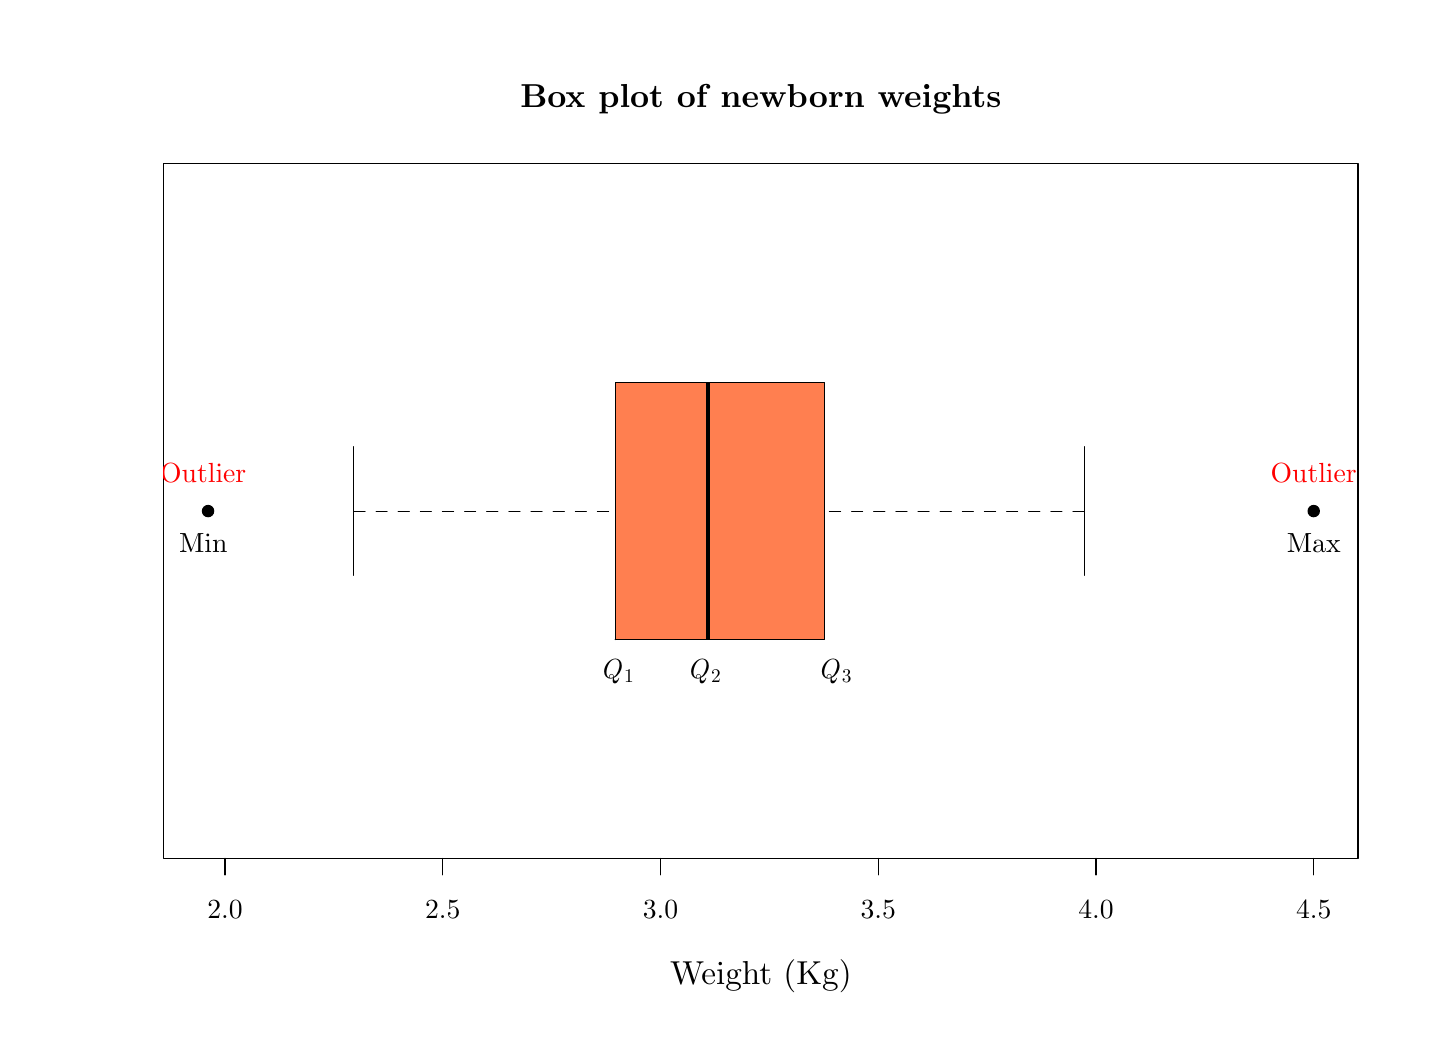
\begin{tikzpicture}[x=1pt,y=1pt]
\definecolor{fillColor}{RGB}{255,255,255}
\path[use as bounding box,fill=fillColor,fill opacity=0.00] (0,0) rectangle (505.89,361.35);
\begin{scope}
\path[clip] ( 49.20, 61.20) rectangle (480.69,312.15);
\definecolor{fillColor}{RGB}{255,127,80}

\path[fill=fillColor] (212.32,140.20) --
	(212.32,233.15) --
	(287.95,233.15) --
	(287.95,140.20) --
	cycle;
\definecolor{drawColor}{RGB}{0,0,0}

\path[draw=drawColor,line width= 1.2pt,line join=round] (245.85,140.20) -- (245.85,233.15);

\path[draw=drawColor,line width= 0.4pt,dash pattern=on 4pt off 4pt ,line join=round,line cap=round] (117.89,186.67) -- (212.32,186.67);

\path[draw=drawColor,line width= 0.4pt,dash pattern=on 4pt off 4pt ,line join=round,line cap=round] (381.73,186.67) -- (287.95,186.67);

\path[draw=drawColor,line width= 0.4pt,line join=round,line cap=round] (117.89,163.44) -- (117.89,209.91);

\path[draw=drawColor,line width= 0.4pt,line join=round,line cap=round] (381.73,163.44) -- (381.73,209.91);

\path[draw=drawColor,line width= 0.4pt,line join=round,line cap=round] (212.32,140.20) --
	(212.32,233.15) --
	(287.95,233.15) --
	(287.95,140.20) --
	(212.32,140.20);
\definecolor{fillColor}{RGB}{0,0,0}

\path[fill=fillColor] ( 65.18,186.67) circle (  2.25);

\path[fill=fillColor] (464.71,186.67) circle (  2.25);
\end{scope}
\begin{scope}
\path[clip] (  0.00,  0.00) rectangle (505.89,361.35);
\definecolor{drawColor}{RGB}{0,0,0}

\path[draw=drawColor,line width= 0.4pt,line join=round,line cap=round] ( 71.31, 61.20) -- (464.71, 61.20);

\path[draw=drawColor,line width= 0.4pt,line join=round,line cap=round] ( 71.31, 61.20) -- ( 71.31, 55.20);

\path[draw=drawColor,line width= 0.4pt,line join=round,line cap=round] (149.99, 61.20) -- (149.99, 55.20);

\path[draw=drawColor,line width= 0.4pt,line join=round,line cap=round] (228.67, 61.20) -- (228.67, 55.20);

\path[draw=drawColor,line width= 0.4pt,line join=round,line cap=round] (307.35, 61.20) -- (307.35, 55.20);

\path[draw=drawColor,line width= 0.4pt,line join=round,line cap=round] (386.03, 61.20) -- (386.03, 55.20);

\path[draw=drawColor,line width= 0.4pt,line join=round,line cap=round] (464.71, 61.20) -- (464.71, 55.20);

\node[text=drawColor,anchor=base,inner sep=0pt, outer sep=0pt, scale=  1.00] at ( 71.31, 39.60) {2.0};

\node[text=drawColor,anchor=base,inner sep=0pt, outer sep=0pt, scale=  1.00] at (149.99, 39.60) {2.5};

\node[text=drawColor,anchor=base,inner sep=0pt, outer sep=0pt, scale=  1.00] at (228.67, 39.60) {3.0};

\node[text=drawColor,anchor=base,inner sep=0pt, outer sep=0pt, scale=  1.00] at (307.35, 39.60) {3.5};

\node[text=drawColor,anchor=base,inner sep=0pt, outer sep=0pt, scale=  1.00] at (386.03, 39.60) {4.0};

\node[text=drawColor,anchor=base,inner sep=0pt, outer sep=0pt, scale=  1.00] at (464.71, 39.60) {4.5};
\end{scope}
\begin{scope}
\path[clip] (  0.00,  0.00) rectangle (505.89,361.35);
\definecolor{drawColor}{RGB}{0,0,0}

\node[text=drawColor,anchor=base,inner sep=0pt, outer sep=0pt, scale=  1.20] at (264.94,332.61) {\bfseries Box plot of newborn weights};

\node[text=drawColor,anchor=base,inner sep=0pt, outer sep=0pt, scale=  1.20] at (264.94, 15.60) {Weight (Kg)};
\end{scope}
\begin{scope}
\path[clip] (  0.00,  0.00) rectangle (505.89,361.35);
\definecolor{drawColor}{RGB}{0,0,0}

\path[draw=drawColor,line width= 0.4pt,line join=round,line cap=round] ( 49.20, 61.20) --
	(480.69, 61.20) --
	(480.69,312.15) --
	( 49.20,312.15) --
	( 49.20, 61.20);
\end{scope}
\begin{scope}
\path[clip] ( 49.20, 61.20) rectangle (480.69,312.15);
\definecolor{drawColor}{RGB}{0,0,0}

\node[text=drawColor,anchor=base west,inner sep=0pt, outer sep=0pt, scale=  1.00] at (206.83,126.11) {\itshape Q};

\node[text=drawColor,anchor=base west,inner sep=0pt, outer sep=0pt, scale=  0.70] at (215.53,124.61) {1};

\node[text=drawColor,anchor=base west,inner sep=0pt, outer sep=0pt, scale=  1.00] at (238.31,126.11) {\itshape Q};

\node[text=drawColor,anchor=base west,inner sep=0pt, outer sep=0pt, scale=  0.70] at (247.00,124.61) {2};

\node[text=drawColor,anchor=base west,inner sep=0pt, outer sep=0pt, scale=  1.00] at (285.51,126.11) {\itshape Q};

\node[text=drawColor,anchor=base west,inner sep=0pt, outer sep=0pt, scale=  0.70] at (294.21,124.61) {3};

\node[text=drawColor,anchor=base,inner sep=0pt, outer sep=0pt, scale=  1.00] at ( 63.44,171.61) {Min};

\node[text=drawColor,anchor=base,inner sep=0pt, outer sep=0pt, scale=  1.00] at (464.71,171.61) {Max};
\definecolor{drawColor}{RGB}{255,0,0}

\node[text=drawColor,anchor=base,inner sep=0pt, outer sep=0pt, scale=  1.00] at ( 63.44,197.17) {Outlier};

\node[text=drawColor,anchor=base,inner sep=0pt, outer sep=0pt, scale=  1.00] at (464.71,197.17) {Outlier};
\end{scope}
\end{tikzpicture}
}
\end{center}
\end{frame}


%---------------------------------------------------------------------slide----
\begin{frame}
\frametitle{Box plot construction}
To create a box plot follow the steps below
\begin{enumerate}
\item Calculate the quartiles. 
\item Draw a box from the lower to the upper quartile. 
\item Split the box with the median or second quartile. 
\item For the whiskers calculate first two values called \emph{fences} $f_1$ y $f_2$. The lower fence is the
lower quartile minus one and a half the interquartile range, and the upper fence is the upper quartile plus one and a
half the interquartile range:
\begin{align*}
f_1&=Q_1-1.5\,\text{IQR}\\
f_2&=Q_3+1.5\,\text{IQR}
\end{align*}
The fences define the interval where data are considered normal.
Any value outside that interval is considered an outlier. \\ 
For the lower whisker draw a segment from the lower quartile to the lower value in the sample grater than or
equal to $f_1$, and for the upper whisker draw a segment from the upper quartile to the highest value in the sample lower than
or equal to $f_2$.
\item Finally, if there are some outlier, draw a dot in every outlier. 
\end{enumerate}
\end{frame}


%---------------------------------------------------------------------slide----
\begin{frame}
\frametitle{Box plot construction}
\framesubtitle{Example of number of children}
\begin{enumerate}
\uncover<2->{\item Calculate the quartiles: $Q_1=1$ children} \uncover<3->{and $Q_2=Q_3=2$ children}
\uncover<4->{\item Draw the box.}
\uncover<5->{\item Calculate the fences $f_1=1-1.5*1=-0.5$ and $f_2=2+1.5*1=3.5$.}
\uncover<6->{\item Draw the whiskers: $w_1=0$ children} \uncover<7->{and $w_2=3$ children.}
\uncover<8->{\item Draw the outliers: 4 children.}
\end{enumerate}
\begin{center}
\scalebox{0.45}{% Created by tikzDevice version 0.8.1 on 2015-11-15 21:50:56
% !TEX encoding = UTF-8 Unicode
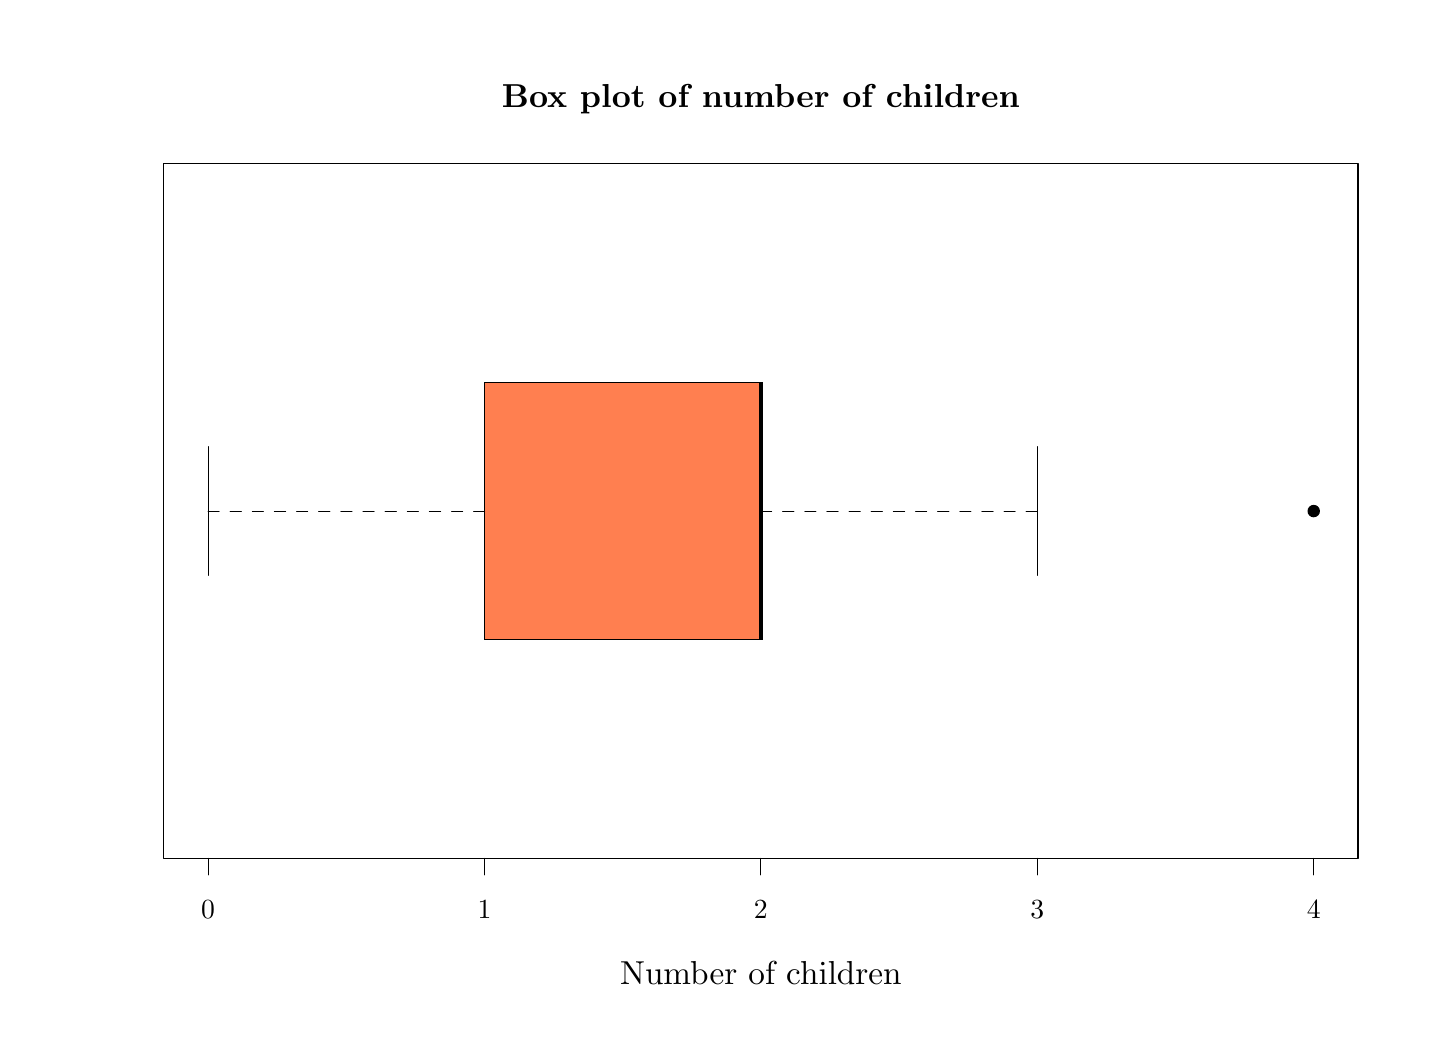
\begin{tikzpicture}[x=1pt,y=1pt]
\definecolor{fillColor}{RGB}{255,255,255}
\path[use as bounding box,fill=fillColor,fill opacity=0.00] (0,0) rectangle (505.89,361.35);
\path[draw,line width= 0.4pt,line join=round,line cap=round] ( 49.20, 61.20) --  (480.69, 61.20) --(480.69,312.15) -- (
49.20,312.15) -- ( 49.20, 61.20); 
\node[anchor=base,inner sep=0pt, outer sep=0pt, scale=  1.20] at (264.94,332.61) {\bfseries Box plot of number of children};
\node[anchor=base,inner sep=0pt, outer sep=0pt, scale=  1.20] at (264.94, 15.60) {Number of children};
\path[draw,line width= 0.4pt,line join=round,line cap=round] ( 65.18, 61.20) -- (464.71, 61.20);
\path[draw,line width= 0.4pt,line join=round,line cap=round] ( 65.18, 61.20) -- ( 65.18, 55.20);
\path[draw,line width= 0.4pt,line join=round,line cap=round] (165.06, 61.20) -- (165.06, 55.20);
\path[draw,line width= 0.4pt,line join=round,line cap=round] (264.94, 61.20) -- (264.94, 55.20);
\path[draw,line width= 0.4pt,line join=round,line cap=round] (364.83, 61.20) -- (364.83, 55.20);
\path[draw,line width= 0.4pt,line join=round,line cap=round] (464.71, 61.20) -- (464.71, 55.20);
\node[anchor=base,inner sep=0pt, outer sep=0pt, scale=  1.00] at ( 65.18, 39.60) {0};
\node[anchor=base,inner sep=0pt, outer sep=0pt, scale=  1.00] at (165.06, 39.60) {1};
\node[anchor=base,inner sep=0pt, outer sep=0pt, scale=  1.00] at (264.94, 39.60) {2};
\node[anchor=base,inner sep=0pt, outer sep=0pt, scale=  1.00] at (364.83, 39.60) {3};
\node[anchor=base,inner sep=0pt, outer sep=0pt, scale=  1.00] at (464.71, 39.60) {4};
\begin{scope}
\path[clip] ( 49.20, 61.20) rectangle (480.69,312.15);
\pause
\definecolor{fillColor}{RGB}{255,127,80}
\path[draw] (165.06,140.20) -- (165.06,233.15);
\pause
\path[draw] (264.94,233.15) --	(264.94,140.20);
\pause
\path[draw, fill=fillColor] (165.06,140.20) -- (165.06,233.15) --	(264.94,233.15) --	(264.94,140.20) --	cycle;
\path[draw,line width= 1.2pt,line join=round] (264.94,140.20) -- (264.94,233.15);
\pause
\pause
\path[draw,line width= 0.4pt,line join=round,line cap=round] ( 65.18,163.44) -- ( 65.18,209.91);
\path[draw,line width= 0.4pt,dash pattern=on 4pt off 4pt ,line join=round,line cap=round] ( 65.18,186.67) -- (165.06,186.67);
\pause
\path[draw,line width= 0.4pt,dash pattern=on 4pt off 4pt ,line join=round,line cap=round] (364.83,186.67) -- (264.94,186.67);
\path[draw,line width= 0.4pt,line join=round,line cap=round] (364.83,163.44) -- (364.83,209.91);
\pause
\path[fill] (464.71,186.67) circle (  2.25);
\end{scope}
\pause
\end{tikzpicture}
}
\end{center}
\end{frame}


%---------------------------------------------------------------------slide----
\begin{frame}
\frametitle{Deviations from the mean}
Another way of measuring spread of data is with respect to a central tendency measure, as for example the mean. 

In that case, it's measured the distance from every value in the sample to the mean, that is called
\structure{\textbf{deviation from the mean.}}

\begin{center}
\scalebox{1}{% Author: Alfredo Sánchez Alberca (email:asalber@ceu.es)
% Plot with the interquartile range
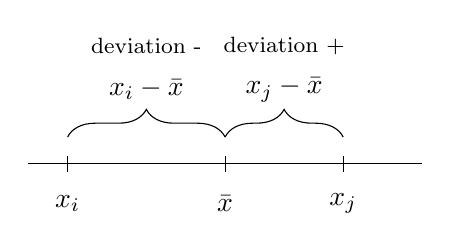
\begin{tikzpicture}[every label/.style={text=color1}]
\draw (0,1) -- (5,1);
\draw (2.5,0.9) -- (2.5,1.1);
\node at (2.5,0.5) {$\bar x$};
\draw (0.5,0.9) -- (0.5,1.1);
\node at (0.5,0.5) {$x_i$}; 
\draw (4,0.9) -- (4,1.1);
\node at (4,0.5) {$x_j$};  
\draw [decorate,decoration={brace,amplitude=10pt},yshift=4pt] (0.5,1.2) -- (2.5,1.2) node
[black,midway,yshift=0.6cm] {$x_i-\bar x$};
\draw [decorate,decoration={brace,amplitude=10pt},yshift=4pt] (2.5,1.2) -- (4,1.2) node
[black,midway,yshift=0.6cm] {$x_j-\bar x$};
\node at (1.5,2.5) {\footnotesize deviation -};
\node at (3.25,2.5) {\footnotesize deviation +};
\end{tikzpicture}}
\end{center}

If deviations are big, the mean would be less representative as when they are small.
%\begin{center} 
%\emph{Which mean is more representative?}
%\end{center}
\end{frame}


%---------------------------------------------------------------------slide----
\begin{frame}
\frametitle{Variance and standard deviation}
\begin{definition}[Sample variance $s^2$]
The \emph{sample variance} of a variable $X$ is the average of squared deviations from the mean. 
\[
s^2 = \frac{\sum (x_i-\bar x)^2n_i}{n} = \sum (x_i-\bar x)^2f_i
\]
\end{definition}
It can also be calculated with the formula
\[
s^2 = \frac{\sum x_i^2n_i}{n} -\bar x^2= \sum x_i^2f_i-\bar x^2
\]
The variance has the units of the variable squared, and to ease their interpretation it's common to calculate its square
root.

\begin{definition}[Sample standard deviation $s$]
The \emph{sample standard deviation} of a variable $X$ is the square root of the variance.
\[
s = +\sqrt{s^2}
\]
\end{definition}
\end{frame}


% %---------------------------------------------------------------------slide----
% \begin{frame}
% \frametitle{Interpretación de la varianza y la desviación típica}
% Tanto la varianza como la desviación típica sirven para cuantificar la dispersión de los datos en torno a la media. 
% %Si la dispersión es grande la media será menos representativa de la muestra que si la dispersión es pequeña.
% \begin{center}
% \includegraphics[scale=0.4]{img/descriptive/interpretacion_varianza}
% 
% %\emph{¿En qué caso es más representativa la media?}
% \end{center}
% 
% \note{Tanto la varianza como la desviación típica sirven para cuantificar la dispersión de los datos en torno a la media. Si la dispersion
% con respecto a la media es pequeña, los individuos se parecerán bastante a la media y esta será más representativa que cuando los
% individuos no se parezcana ella y la dispersión con respecto a la media sea mayor.}
% \end{frame}
% 
% 
%---------------------------------------------------------------------slide----
\begin{frame}
\frametitle{Variance and standard deviation calculation}
\framesubtitle{Example with non-grouped data}
Using the data of the sample with the number of children of families, and adding a new column to the frequency table
with the squared values, 
\[
\setlength\arraycolsep{3mm}
\setlength\arrayrulewidth{0.5pt}
\begin{array}{rrr}
\hline
\multicolumn{1}{c}{x_i} & \multicolumn{1}{c}{n_i} & \multicolumn{1}{c}{x_i^2n_i} \\
\hline
0 & 2 & 0 \\
1 & 6 & 6 \\
2 & 14 & 56\\
3 & 2  & 18\\
4 & 1 & 16 \\
\hline
\sum & 25 & 96 \\
\hline
\end{array}
\]
\[
s^2 = \frac{\sum x_i^2n_i}{n}-\bar x^2 = \frac{96}{25}-1.76^2= 0.7424 \mbox{ children}^2.
\]
and the standard deviation is $s=\sqrt{0.7424} = 0.8616$ children.

Compared to the range, that is 4 children, the standard deviation is not very large, so we can conclude
that the dispersion of the distribution is small and consequently the mean, $\bar x=1.76$ children, represents quite
well the number of children of families of the sample. 
\end{frame}


% %---------------------------------------------------------------------slide----
% \begin{frame}
% \frametitle{Cálculo de la varianza y la desviación típica}
% \framesubtitle{Ejemplo con datos agrupados}
% En el ejemplo de las estaturas, al ser datos agrupados, el cálculo se realiza igual que antes pero tomando como valores de la variable las
% marcas de clase. 
% \begin{center}
% \setlength\arraycolsep{3mm}
% \setlength\arrayrulewidth{0.5pt}
% \begin{array}{rrrr}
% \hline
% \multicolumn{1}{c}{X} & \multicolumn{1}{c}{x_i} & \multicolumn{1}{c}{n_i} & \multicolumn{1}{c}{x_i^2n_i} \\
% \hline
% (150,160] & 155 & 2 & 48050\\
% (160,170] & 165 & 8 & 217800\\
% (170,180] & 175 & 11 & 336875\\
% (180,190] & 185 & 7 & 239575\\
% (190,200] & 195 & 2 & 76050\\ 
% \hline 
% \sum &  & 30 & 918350 \\
% \hline
% \end{array}
% \end{center}
% \[
% s^2 = \frac{\sum x_i^2n_i}{n}-\bar x^2 = \frac{918350}{30}-174.67^2= 102.06 \mbox{ cm}^2.
% \]
% Y la desviación típica es $s=\sqrt{102.06} = 10.1$ cm.
% 
% Este valor es bastante pequeño, comparado con el recorrido de la variable, que va de 150 a 200 cm, por lo que la variable tiene poca
% dispersión y en consecuencia su media es muy representativa.
% 
% \note{En el ejemplo de las estaturas, como se habían agrupado los datos, como valores se tomarán las
% marcas de clases, es decir, 155 elevado al cuadrado y por su frecuencia absoluta que es 2, lo que nos da 48050, y así sucesivamente. Después
% hay que sumar los valores de esta columna y dividirlos por el tamaño de la muestra que era 30. Finalmente al cociente se le resta el valor
% de la media que era $174.67$ elevada al cuadrado, lo que nos da 102.06 cm al cuadrado.
% 
% Si sacamos la raíz cuadrada se obtiene una desviación típica de 10.1 cm, que es un valor pequeño comparado con el recorrido de la variable
% que va de 150 a 200 cm, por lo que se puede concluir que la muestra tiene poca dispersión y por tanto la media representa muy bien al resto
% de individuos de la muestra.}
% \end{frame}
% 
% 
% %---------------------------------------------------------------------slide----
% \begin{frame}
% \frametitle{Coeficiente de variación}
% Tanto la varianza como la desviación típica tienen unidades y eso dificulta a veces su interpretación y su comparación.
% 
% Afortunadamente es fácil definir a partir de ellas una medida de dispersión adimensional que es más fácil de interpretar.
% \begin{definition}[Coeficiente de variación muestral $cv$]
% El \emph{coeficiente de variación muestral} de una variable $X$ se define como el cociente entre su desviación típica muestral y el valor absoluto de su media muestral.
% \[
% cv = \frac{s}{|\bar x|}
% \]
% \end{definition}
% El coeficiente de variación muestral mide la dispersión relativa de los valores de la muestra en torno a la media muestral.
%  
% Como no tiene unidades, es muy sencillo de interpretar: Cuanto mayor sea, mayor será la dispersión y menos
% representativa será la media.
% 
% También se utiliza para comparar la dispersión entre muestras distintas incluso si las variables tienen unidades diferentes.
% \begin{center}
% \alert{\emph{¡Ojo! No tiene sentido cuando la media muestral vale 0 o valores próximos.}}
% \end{center}
% 
% \note{Tanto la varianza como la desviación típica tienen unidades lo que dificulta a veces su interpretación.
% 
% Afortunadamente es fácil definir a partir de ellas una medida de dispersión adimensional que es más fácil de interpretar.
% 
% El coeficiente de variación muestral, que se representa mediante cv, se defiene como el cociente entre la desviación típica y el valor
% absoluto de la media.
% 
% Como tanto la desviación típica como la media tienen las unidades de la variable, al hacer su cociente las unidades desaparecen y se obtiene
% una medida adimensional que resulta más sencilla de interpretar. 
% 
% Al estar dividido por el valor absoluto de la media, el coeficiente de variación mide la dispersión relativa de los valores de la muestra
% en torno a la media muestral, y como en el numerador está la desviación típica, cuanto mayor sea esta, mayor será el coeficiente de
% variación y por tanto mayor será la dispersión relativa de la variable en torno a la media.
% 
% Una de las principales utilidades del coeficiente de variación es que, precisamente por no tener unidades, permite la comparación de la
% dispersión de muestras distintas, incluso si son de variables con distintas unidades. 
% 
% El único problema de este estadístico es que no vale cuando la media muestral vale 0 o próxima a 0, ya que al estar en el denominador,
% obtendríamos valores muy grandes.}
% \end{frame}
% 
% 
% %---------------------------------------------------------------------slide----
% \begin{frame}
% \frametitle{Coeficiente de variación}
% \framesubtitle{Ejemplo}
% En el caso del número de hijos, como $\bar x=1.76$ hijos y $s=0.8616$ hijos, se tiene que el coefiente de variación vale
% \[
% cv = \frac{s}{|\bar x|} = \frac{0.8616}{|1.76|} = 0.49.
% \]
% En el caso de las estaturas, como $\bar x=174.67$ cm y $s=10.1$ cm, se tiene que el coeficiente de variación vale 
% \[
% cv = \frac{s}{|\bar x|} = \frac{10.1}{|174.67|} = 0.06.
% \]
% Como se puede observar la dispersión relativa en la muestra de estaturas es mucho menor que en la del número de hijos, por lo que la media
% de las estaturas será más representativa que la media del número de hijos. 
% \end{frame}
% 
% 
% \subsection{Estadísticos de forma}
% %---------------------------------------------------------------------slide----
% \begin{frame}
% \frametitle{Estadísticos de forma}
% Son medidas que tratan de caracterizar aspectos de la forma de la distribución de una muestra.
% 
% Los aspectos más relevantes son:
% \begin{description}
% \item[Simetría:] Miden la simetría de la distribución de frecuencias en torno a la media.\\
% El estadístico más utilizado es el \emph{Coeficiente de Asimetría de Fisher}.
% \item[Apuntamiento:] Miden el apuntamiento de la distribución de frecuencias.\\
% El estadístico más utilizado es el \emph{Coeficiente de Apuntamiento o Curtosis}.
% \end{description}
% \note{Los estadísticos de forma se encargan de describir, como su propio nombre indica, la forma que tiene la distribución de valores en la
% muestra, en particular se estudian dos aspectos que son la asímetría y el apuntamiento.}
% \end{frame}
% 
% 
% %---------------------------------------------------------------------slide----
% \begin{frame}
% \frametitle{Coeficiente de asimetría}
% \begin{definition}[Coeficiente de asimetría muestral $g_1$]
% El \emph{coeficiente de asimetría muestral} de una variable $X$ se define como el promedio de las desviaciones de los
% valores de la muestra respecto de la media muestral, elevadas al cubo, dividido por la desviación típica al cubo. \[g_1
% = \frac{\sum (x_i-\bar x)^3 n_i/n}{s^3} = \frac{\sum (x_i-\bar x)^3 f_i}{s^3}\]
% \end{definition}
% El coeficiente de asimetría muestral mide el grado de simetría de los valores de la muestra con respecto a la media muestral, de manera que:
% \begin{itemize}
% \item $g_1=0$ indica que hay el mismo número de valores a la derecha y a la izquierda de la media (simétrica).
% \item $g_1<0$ indica que la mayoría de los valores son mayores que la media (asimétrica a la izquierda).
% \item $g_1>0$ indica que la mayoría de los valores son menores que la media (asimétrica a la derecha).
% \end{itemize}
% 
% \note{La simetría con respecto a la media tiene que ver con la ubicación de los valores a un lado y otro de la media, cuántos valores hay
% por encima y cuántos por debajo, y cómo están de alejados.
% 
% El coeficiente de asimetría muestral, que se representa $g_1$ se define, como la suma del producto de las desviaciones de los valores de la
% muestra a la media muestral elevadas al cubo por su frecuencia absoluta, dividida por el tamaño de la muestra, y a su vez todo dividido
% por la desviación típica al cubo.
% 
% Como las desviaciones elevadas al cubo tienen las unidades de la variable al cubo y la desviación típica elevada al cubo también tiene las
% unidades de la variable al cubo, al realizar el cociente las unidades se cancelan y por tanto el coeficiente de asimetría es una medida
% adimensional que mide el grado de asimetría de los valores de la muestra con respecto a la media, de manera que:
% \begin{itemize}
% \item $g_1=0$ indica que hay el mismo número de valores a la derecha y a la izquierda de la media y por tanto la distribución es simétrica.
% \item $g_1<0$ indica que la mayoría de los valores son mayores que la media y entonces se dice que la distribución es asimétrica hacia la
% izquierda.
% \item $g_1>0$ indica que la mayoría de los valores son menores que la media y entonces se dice que la distribución es asimétrica hacia la
% derecha.
% \end{itemize}
% }
% \end{frame}
% 
% 
% %---------------------------------------------------------------------slide----
% \begin{frame}
% \frametitle{Coeficiente de asimetría}
% \framesubtitle{Ejemplo de distribución simétrica}
% \begin{center}
% \scalebox{0.8}{%% Input file name: distribucion_simetrica.fig
%% FIG version: 3.2
%% Orientation: Landscape
%% Justification: Flush Left
%% Units: Inches
%% Paper size: A4
%% Magnification: 100.0
%% Resolution: 1200ppi
%% Include the following in the preamble:
%% \usepackage{textcomp}
%% End

\begin{pspicture}(5.91cm,3.25cm)(17.37cm,13.10cm)
\psset{unit=0.8cm}
%%
%% Depth: 2147483647
%%
\newrgbcolor{mycolor0}{1.00 0.50 0.31}\definecolor{mycolor0}{rgb}{1.00,0.50,0.31}
%%
%% Depth: 100
%%
\rput[l](13.59,15.54){Distribución simétrica \alert{$g_1=0$}}
\rput{90}(9.68,10.89){Frecuencia relativa}
\psset{linestyle=solid,linewidth=0.03175,linecolor=black,fillstyle=none}
\psline(11.04,7.07)(11.04,14.71)
\psline(11.04,7.07)(10.83,7.07)
\psline(11.04,8.98)(10.83,8.98)
\psline(11.04,10.89)(10.83,10.89)
\psline(11.04,12.80)(10.83,12.80)
\psline(11.04,14.71)(10.83,14.71)
\rput{90}(10.53,7.07){0.0}
\rput{90}(10.53,8.98){0.1}
\rput{90}(10.53,10.89){0.2}
\rput{90}(10.53,12.80){0.3}
\rput{90}(10.53,14.71){0.4}
\psset{fillstyle=solid,fillcolor=mycolor0}
\pspolygon(10.74,7.07)(10.74,7.07)(11.42,7.07)(11.42,7.07)(10.74,7.07)
\pspolygon(11.42,7.07)(11.42,7.11)(12.09,7.11)(12.09,7.07)(11.42,7.07)
\pspolygon(12.09,7.07)(12.09,7.25)(12.76,7.25)(12.76,7.07)(12.09,7.07)
\pspolygon(12.76,7.07)(12.76,7.69)(13.43,7.69)(13.43,7.07)(12.76,7.07)
\pspolygon(13.43,7.07)(13.43,8.75)(14.10,8.75)(14.10,7.07)(13.43,7.07)
\pspolygon(14.10,7.07)(14.10,10.56)(14.77,10.56)(14.77,7.07)(14.10,7.07)
\pspolygon(14.77,7.07)(14.77,12.83)(15.45,12.83)(15.45,7.07)(14.77,7.07)
\pspolygon(15.45,7.07)(15.45,14.38)(16.12,14.38)(16.12,7.07)(15.45,7.07)
\pspolygon(16.12,7.07)(16.12,14.36)(16.79,14.36)(16.79,7.07)(16.12,7.07)
\pspolygon(16.79,7.07)(16.79,12.80)(17.46,12.80)(17.46,7.07)(16.79,7.07)
\pspolygon(17.46,7.07)(17.46,10.58)(18.14,10.58)(18.14,7.07)(17.46,7.07)
\pspolygon(18.14,7.07)(18.14,8.75)(18.81,8.75)(18.81,7.07)(18.14,7.07)
\pspolygon(18.81,7.07)(18.81,7.70)(19.48,7.70)(19.48,7.07)(18.81,7.07)
\pspolygon(19.48,7.07)(19.48,7.26)(20.15,7.26)(20.15,7.07)(19.48,7.07)
\pspolygon(20.15,7.07)(20.15,7.11)(20.82,7.11)(20.82,7.07)(20.15,7.07)
\pspolygon(20.82,7.07)(20.82,7.07)(21.20,7.07)(21.20,7.07)(20.82,7.07)
\rput[l](16.03,6.5){$\bar x$}
\psset{linewidth=0.0635,fillstyle=none}
\psline(16.12,4.58)(16.12,5.76)
\psset{linestyle=dashed,linewidth=0.03175}
\psline(13.48,5.17)(15.46,5.17)
\psline(18.75,5.17)(16.78,5.17)
\psset{linestyle=solid}
\psline(13.48,4.88)(13.48,5.47)
\psline(18.75,4.88)(18.75,5.47)
\psline(15.46,4.58)(15.46,5.76)(16.78,5.76)(16.78,4.58)(15.46,4.58)
\end{pspicture}
%% End
}
% \end{center}
% \note{Aquí tenemos el histograma de una distribución simétrica. Como puede observarse, la media queda justo en el centro de la
% distribución, coincidiendo con la mediana y existe el mismo número de barras y con la misma frecuencia a un lado y a otro de la media.}
% \end{frame}
% 
% 
% %---------------------------------------------------------------------slide----
% \begin{frame}
% \frametitle{Coeficiente de asimetría}
% \framesubtitle{Ejemplo de distribución asimétrica hacia la izquierda}
% \begin{center}
% \scalebox{0.8}{%% Input file name: distribucion_asimetrica_izquierda.fig
%% FIG version: 3.2
%% Orientation: Landscape
%% Justification: Flush Left
%% Units: Inches
%% Paper size: A4
%% Magnification: 100.0
%% Resolution: 1200ppi
%% Include the following in the preamble:
%% \usepackage{textcomp}
%% End

\begin{pspicture}(5.91cm,3.25cm)(17.07cm,13.10cm)
\psset{unit=0.8cm}
%%
%% Depth: 2147483647
%%
\newrgbcolor{mycolor0}{1.00 0.50 0.31}\definecolor{mycolor0}{rgb}{1.00,0.50,0.31}
%%
%% Depth: 100
%%
\rput[l](12.07,15.54){Distribución asimétrica a la izquierda \alert{$g_1<0$}}
\rput{90}(9.68,10.89){Frecuencia relativa}
\psset{linestyle=solid,linewidth=0.03175,linecolor=black,fillstyle=none}
\psline(11.04,7.07)(11.04,14.71)
\psline(11.04,7.07)(10.83,7.07)
\psline(11.04,8.34)(10.83,8.34)
\psline(11.04,9.61)(10.83,9.61)
\psline(11.04,10.89)(10.83,10.89)
\psline(11.04,12.16)(10.83,12.16)
\psline(11.04,13.44)(10.83,13.44)
\psline(11.04,14.71)(10.83,14.71)
\rput{90}(10.53,7.07){0.00}
\rput{90}(10.53,8.34){0.02}
\rput{90}(10.53,9.61){0.04}
\rput{90}(10.53,10.89){0.06}
\rput{90}(10.53,12.16){0.08}
\rput{90}(10.53,13.44){0.10}
\rput{90}(10.53,14.71){0.12}
\psset{fillstyle=solid,fillcolor=mycolor0}
\pspolygon(10.79,7.07)(10.79,7.07)(11.42,7.07)(11.42,7.07)(10.79,7.07)
\pspolygon(11.42,7.07)(11.42,7.08)(12.04,7.08)(12.04,7.07)(11.42,7.07)
\pspolygon(12.04,7.07)(12.04,7.08)(12.67,7.08)(12.67,7.07)(12.04,7.07)
\pspolygon(12.67,7.07)(12.67,7.11)(13.30,7.11)(13.30,7.07)(12.67,7.07)
\pspolygon(13.30,7.07)(13.30,7.15)(13.92,7.15)(13.92,7.07)(13.30,7.07)
\pspolygon(13.92,7.07)(13.92,7.24)(14.55,7.24)(14.55,7.07)(13.92,7.07)
\pspolygon(14.55,7.07)(14.55,7.42)(15.18,7.42)(15.18,7.07)(14.55,7.07)
\pspolygon(15.18,7.07)(15.18,7.75)(15.81,7.75)(15.81,7.07)(15.18,7.07)
\pspolygon(15.81,7.07)(15.81,8.32)(16.43,8.32)(16.43,7.07)(15.81,7.07)
\pspolygon(16.43,7.07)(16.43,9.29)(17.06,9.29)(17.06,7.07)(16.43,7.07)
\pspolygon(17.06,7.07)(17.06,10.70)(17.69,10.70)(17.69,7.07)(17.06,7.07)
\pspolygon(17.69,7.07)(17.69,12.43)(18.31,12.43)(18.31,7.07)(17.69,7.07)
\pspolygon(18.31,7.07)(18.31,13.85)(18.94,13.85)(18.94,7.07)(18.31,7.07)
\pspolygon(18.94,7.07)(18.94,13.75)(19.57,13.75)(19.57,7.07)(18.94,7.07)
\pspolygon(19.57,7.07)(19.57,11.01)(20.20,11.01)(20.20,7.07)(19.57,7.07)
\pspolygon(20.20,7.07)(20.20,7.67)(20.82,7.67)(20.82,7.07)(20.20,7.07)
\rput[l](18.22,6.5){$\bar x$}
\psset{linewidth=0.0635,fillstyle=none}
\psline(19.34,4.58)(19.34,5.76)
\psset{linestyle=dashed,linewidth=0.03175}
\psline(17.19,5.17)(18.76,5.17)
\psline(20.82,5.17)(19.80,5.17)
\psset{linestyle=solid}
\psline(17.19,4.88)(17.19,5.47)
\psline(20.82,4.88)(20.82,5.47)
\psline(18.76,4.58)(18.76,5.76)(19.80,5.76)(19.80,4.58)(18.76,4.58)
\end{pspicture}
%% End
}
% \end{center}
% \note{En este otro caso tenemos una distribución asimétrica hacia la izquierda, donde la media queda por debajo de la mediana y las barras
% son más altas a la derecha de la media, lo que indica que hay más valores por encima de la media. Por debajo de la media habría menos
% valores, barras más bajas, pero más alejados.}
% \end{frame}
% 
% 
% %---------------------------------------------------------------------slide----
% \begin{frame}
% \frametitle{Coeficiente de asimetría}
% \framesubtitle{Ejemplo de distribución asimétrica hacia la derecha}
% \begin{center}
% \scalebox{0.8}{%% Input file name: distribucion_asimetrica_derecha.fig
%% FIG version: 3.2
%% Orientation: Landscape
%% Justification: Flush Left
%% Units: Inches
%% Paper size: A4
%% Magnification: 100.0
%% Resolution: 1200ppi
%% Include the following in the preamble:
%% \usepackage{textcomp}
%% End

\begin{pspicture}(5.91cm,3.25cm)(17.37cm,13.10cm)
\psset{unit=0.8cm}
%%
%% Depth: 2147483647
%%
\newrgbcolor{mycolor0}{1.00 0.50 0.31}\definecolor{mycolor0}{rgb}{1.00,0.50,0.31}
%%
%% Depth: 100
%%
\rput[l](12.16,15.54){Distribución asimétrica a la derecha \alert{$g_1>0$}}
\rput{90}(9.68,10.89){Frecuencia relativa}
\psset{linestyle=solid,linewidth=0.03175,linecolor=black,fillstyle=none}
\psline(11.04,7.07)(11.04,14.71)
\psline(11.04,7.07)(10.83,7.07)
\psline(11.04,8.34)(10.83,8.34)
\psline(11.04,9.61)(10.83,9.61)
\psline(11.04,10.89)(10.83,10.89)
\psline(11.04,12.16)(10.83,12.16)
\psline(11.04,13.44)(10.83,13.44)
\psline(11.04,14.71)(10.83,14.71)
\rput{90}(10.53,7.07){0.00}
\rput{90}(10.53,8.34){0.02}
\rput{90}(10.53,9.61){0.04}
\rput{90}(10.53,10.89){0.06}
\rput{90}(10.53,12.16){0.08}
\rput{90}(10.53,13.44){0.10}
\rput{90}(10.53,14.71){0.12}
\psset{fillstyle=solid,fillcolor=mycolor0}
\pspolygon(11.42,7.07)(11.42,7.67)(12.04,7.67)(12.04,7.07)(11.42,7.07)
\pspolygon(12.04,7.07)(12.04,11.02)(12.67,11.02)(12.67,7.07)(12.04,7.07)
\pspolygon(12.67,7.07)(12.67,13.76)(13.30,13.76)(13.30,7.07)(12.67,7.07)
\pspolygon(13.30,7.07)(13.30,13.85)(13.92,13.85)(13.92,7.07)(13.30,7.07)
\pspolygon(13.92,7.07)(13.92,12.43)(14.55,12.43)(14.55,7.07)(13.92,7.07)
\pspolygon(14.55,7.07)(14.55,10.70)(15.18,10.70)(15.18,7.07)(14.55,7.07)
\pspolygon(15.18,7.07)(15.18,9.29)(15.81,9.29)(15.81,7.07)(15.18,7.07)
\pspolygon(15.81,7.07)(15.81,8.32)(16.43,8.32)(16.43,7.07)(15.81,7.07)
\pspolygon(16.43,7.07)(16.43,7.74)(17.06,7.74)(17.06,7.07)(16.43,7.07)
\pspolygon(17.06,7.07)(17.06,7.41)(17.69,7.41)(17.69,7.07)(17.06,7.07)
\pspolygon(17.69,7.07)(17.69,7.24)(18.31,7.24)(18.31,7.07)(17.69,7.07)
\pspolygon(18.31,7.07)(18.31,7.15)(18.94,7.15)(18.94,7.07)(18.31,7.07)
\pspolygon(18.94,7.07)(18.94,7.11)(19.57,7.11)(19.57,7.07)(18.94,7.07)
\pspolygon(19.57,7.07)(19.57,7.09)(20.20,7.09)(20.20,7.07)(19.57,7.07)
\pspolygon(20.20,7.07)(20.20,7.07)(20.82,7.07)(20.82,7.07)(20.20,7.07)
\pspolygon(20.82,7.07)(20.82,7.07)(21.20,7.07)(21.20,7.07)(20.82,7.07)
\rput[l](13.83,6.5){$\bar x$}
\psset{linewidth=0.0635,fillstyle=none}
\psline(12.96,4.58)(12.96,5.76)
\psset{linestyle=dashed,linewidth=0.03175}
\psline(11.42,5.17)(12.47,5.17)
\psline(15.22,5.17)(13.57,5.17)
\psset{linestyle=solid}
\psline(11.42,4.88)(11.42,5.47)
\psline(15.22,4.88)(15.22,5.47)
\psline(12.47,4.58)(12.47,5.76)(13.57,5.76)(13.57,4.58)(12.47,4.58)
\end{pspicture}
%% End
}
% \end{center}
% \note{Y en este otro caso tenemos una distribución asimétrica hacia la derecha, donde la media queda por encima de la mediana y las barras
% son más altas a la izquierda de la media, lo que indica que hay más valores por debajo de la media. Por encima de la media habría menos
% valores, barras más bajas, pero más alejados.}
% \end{frame}
% 
% 
% %---------------------------------------------------------------------slide----
% \begin{frame}
% \frametitle{Cálculo del coeficiente de asimetría}
% \framesubtitle{Ejemplo con datos agrupados}
% Siguiendo con el ejemplo de las estaturas, podemos calcular el coeficiente de asimetría a partir de la tabla de frecuencias añadiendo una
% nueva columna con los cubos de las desviaciones a la media $\bar x = 174.67$ cm:
% \begin{center}
% \setlength\arraycolsep{3mm}
% \setlength\arrayrulewidth{0.5pt}
% \begin{array}{rrrrr}
% \hline
% \multicolumn{1}{c}{X} & \multicolumn{1}{c}{x_i} & \multicolumn{1}{c}{n_i} & \multicolumn{1}{c}{x_i-\bar x} & \multicolumn{1}{c}{(x_i-\bar x)^3 n_i} \\
% \hline
% (150,160] & 155 & 2 & -19.67 & -15221.00\\
% (160,170] & 165 & 8 & -9.67 & -7233.85\\
% (170,180] & 175 & 11 & 0.33 & 0.40\\
% (180,190] & 185 & 7 & 10.33 & 7716.12\\
% (190,200] & 195 & 2 & 20.33 & 16805.14\\ 
% \hline  
% \sum &  & 30 & & 2066.81 \\
% \hline
% \end{array}
% \end{center}
% \[
% g_1 = \frac{\sum (x_i-\bar x)^3n_i/n}{s^3} = \frac{2066.81/30}{10.1^3} = 0.07.
% \]
% Al estar tan próximo a 0, este valor indica que la distribución es prácticamente simétrica con respecto a la media. 
% 
% \note{Para calcular el coeficiente de asimetría en el ejemplo de las estaturas se puede añadir una nueva columna a la
% tabla de frecuencias con las desviaciones de los valores a la media que recordemos valía $174.67$ cm. Como habíamos agrupado los datos en
% clases, para calcular las desviaciones a la media se toma la marca de cada clase. Así, la primera desviación es 155 menos la media 174.67 lo
% que nos da $-19.67$ cm, la segunda es 165 menos $174.67$ cm y así sucesivamente. Obsérvese que las desviaciones de los valores menos que la
% media serán negativas y que las de los valores mayores serán positivas. A continuación se añade otra columna a la tabla con el producto de
% las desviaciones elevadas al cubo por su frecuencia absoluta, es decir, $-19.67$ al cubo por su frecuencia absoluta que es 2, lo que nos da
% $-15221$, $-9.67$ elevado al cubo y por su frecuencia absoluta que es 8, lo que nos da $-7233.85$, y así sucesivamente. Al final se suman
% los valores de esta columna y se dividen por el tamaño de la muestra que era 30. Por último el resultado de este cociente se vuelve a dividir por la desviación típica
% que era $10.1$ cm elevada al cubo, y se obtiene $0.07$.
% 
% Como este valor está muy próximo a 0, se puede concluir que la distribución de las estaturas es prácticamente simétrica.
% }
% \end{frame}
% 
% 
% %---------------------------------------------------------------------slide----
% \begin{frame}
% \frametitle{Coeficiente de apuntamiento o curtosis}
% \begin{definition}[Coeficiente de apuntamiento muestral $g_2$]
% El \emph{coeficiente de apuntamiento muestral} de una variable $X$ se define como el promedio de las desviaciones de
% los valores de la muestra respecto de la media muestral, elevadas a la cuarta, dividido por la desviación típica a la
% cuarta y al resultado se le resta 3. \[g_2 = \frac{\sum (x_i-\bar x)^4 n_i/n}{s^4}-3 = \frac{\sum (x_i-\bar x)^4 f_i}{s^4}-3\]
% \end{definition}
% El coeficiente de apuntamiento muestral mide el grado de apuntamiento de los valores de la muestra con respecto a una distribución normal de referencia, de manera que:
% \begin{itemize}
% \item $g_2=0$ indica que la distribución tienen un apuntamiento normal (\emph{mesocúrtica}).
% \item $g_2<0$ indica que la distribución tiene menos apuntamiento de lo normal (\emph{platicúrtica}).
% \item $g_2>0$ indica que la distribución tiene más apuntamiento de lo normal (\emph{leptocúrtica}).
% \end{itemize}
% 
% \note{El apuntamiento de una distribución muestral tiene que ver con la pendiente su polígono de frecuencias.
% 
% El coeficiente de apuntamiento o kurtosis muestral, que se representa $g_2$ se define, como la suma del producto de las desviaciones de los
% valores de la muestra a la media muestral elevadas a la cuarta por su frecuencia absoluta, dividida por el tamaño de la muestra, y a su vez
% todo dividido por la desviación típica a la cuarta, y al final se resta 3 al cociente. Como puede verse, la fórmula es muy parecida a la del
% coeficiente de asimetría, pero tomando las potencias cuartas en lugar de las potencias al cubo, y restando 3 al cociente. 
% 
% Al igual que para el coeficiente de asimetría, como las desviaciones elevadas a la cuarta tienen las unidades de la variable a la cuarta y
% la desviación típica elevada al cubo también tiene las unidades de la variable a la cuarta, al realizar el cociente las unidades se cancelan
% y por tanto el coeficiente de apuntamiento es una medida adimensional que mide el grado de apuntamiento de la distribución muestral.
% 
% El apuntamiento suele medirse en comparación con un apuntamiento de referencia que es el de una distribución normal. La distribución normal
% se verá maś adelante en el curso, pero baste decir que es la distribución más común que se presenta en la naturaleza, y por lo tanto, está
% justificado tomarla como referencia y comparar el apuntamiento de cualquier otra distribución con el de la distribución normal que siempre
% vale 0. Por tanto cuando
% \begin{itemize}
% \item $g_2=0$ indica que la distribución tienen un apuntamiento normal (\emph{mesocúrtica}).
% \item $g_2<0$ indica que la distribución tiene menos apuntamiento de lo normal (\emph{platicúrtica}).
% \item $g_2>0$ indica que la distribución tiene más apuntamiento de lo normal (\emph{leptocúrtica}
% \end{itemize}
% }
% \end{frame}
% 
% 
% %---------------------------------------------------------------------slide----
% \begin{frame}
% \frametitle{Coeficiente de apuntamiento o curtosis}
% \framesubtitle{Ejemplo de distribución mesocúrtica}
% \begin{center}
% \scalebox{0.8}{%% Input file name: distribucion_mesocurtica.fig
%% FIG version: 3.2
%% Orientation: Landscape
%% Justification: Flush Left
%% Units: Inches
%% Paper size: A4
%% Magnification: 100.0
%% Resolution: 1200ppi
%% Include the following in the preamble:
%% \usepackage{textcomp}
%% End

\begin{pspicture}(5.26cm,3.44cm)(16.90cm,11.91cm)
\psset{unit=0.8cm}
%%
%% Depth: 2147483647
%%
\newrgbcolor{mycolor0}{1.00 0.50 0.31}\definecolor{mycolor0}{rgb}{1.00,0.50,0.31}
\newrgbcolor{mycolor1}{0.25 0.41 0.88}\definecolor{mycolor1}{rgb}{0.25,0.41,0.88}
%%
%% Depth: 100
%%
\rput[l](12.46,14.06){Distribución mesocúrtica \alert{$g_2=0$}}
\rput{90}(8.88,8.89){Frecuencia relativa}
\psset{linestyle=solid,linewidth=0.03175,linecolor=black,fillstyle=solid,fillcolor=mycolor0}
\pspolygon(9.94,4.82)(9.94,4.83)(10.61,4.83)(10.61,4.82)(9.94,4.82)
\pspolygon(10.61,4.82)(10.61,4.87)(11.27,4.87)(11.27,4.82)(10.61,4.82)
\pspolygon(11.27,4.82)(11.27,5.01)(11.94,5.01)(11.94,4.82)(11.27,4.82)
\pspolygon(11.94,4.82)(11.94,5.49)(12.61,5.49)(12.61,4.82)(11.94,4.82)
\pspolygon(12.61,4.82)(12.61,6.60)(13.27,6.60)(13.27,4.82)(12.61,4.82)
\pspolygon(13.27,4.82)(13.27,8.57)(13.94,8.57)(13.94,4.82)(13.27,4.82)
\pspolygon(13.94,4.82)(13.94,10.92)(14.61,10.92)(14.61,4.82)(13.94,4.82)
\pspolygon(14.61,4.82)(14.61,12.63)(15.27,12.63)(15.27,4.82)(14.61,4.82)
\pspolygon(15.27,4.82)(15.27,12.64)(15.94,12.64)(15.94,4.82)(15.27,4.82)
\pspolygon(15.94,4.82)(15.94,10.93)(16.61,10.93)(16.61,4.82)(15.94,4.82)
\pspolygon(16.61,4.82)(16.61,8.55)(17.27,8.55)(17.27,4.82)(16.61,4.82)
\pspolygon(17.27,4.82)(17.27,6.61)(17.94,6.61)(17.94,4.82)(17.27,4.82)
\pspolygon(17.94,4.82)(17.94,5.49)(18.60,5.49)(18.60,4.82)(17.94,4.82)
\pspolygon(18.60,4.82)(18.60,5.02)(19.27,5.02)(19.27,4.82)(18.60,4.82)
\pspolygon(19.27,4.82)(19.27,4.86)(19.94,4.86)(19.94,4.82)(19.27,4.82)
\pspolygon(19.94,4.82)(19.94,4.83)(20.60,4.83)(20.60,4.82)(19.94,4.82)
\psset{fillstyle=none}
\psline(10.23,4.82)(10.23,12.97)
\psline(10.23,4.82)(10.02,4.82)
\psline(10.23,6.86)(10.02,6.86)
\psline(10.23,8.89)(10.02,8.89)
\psline(10.23,10.93)(10.02,10.93)
\psline(10.23,12.97)(10.02,12.97)
\rput{90}(9.73,4.82){0.0}
\rput{90}(9.73,6.86){0.1}
\rput{90}(9.73,8.89){0.2}
\rput{90}(9.73,10.93){0.3}
\rput{90}(9.73,12.97){0.4}
\psset{linewidth=0.0635,linecolor=mycolor1}
\psline(10.61,4.84)(10.70,4.84)(10.79,4.85)(10.89,4.85)(10.98,4.86)(11.07,4.87)(11.17,4.89)(11.26,4.91)(11.35,4.93)(11.45,4.95)(11.54,4.98)(11.63,5.01)(11.73,5.05)(11.82,5.10)(11.91,5.16)(12.01,5.22)(12.10,5.30)(12.19,5.38)(12.29,5.48)(12.38,5.59)(12.47,5.71)(12.57,5.85)(12.66,6.01)(12.75,6.18)(12.85,6.37)(12.94,6.58)(13.03,6.80)(13.13,7.04)(13.22,7.30)(13.31,7.58)(13.41,7.87)(13.50,8.18)(13.59,8.49)(13.69,8.82)(13.78,9.16)(13.87,9.50)(13.97,9.85)(14.06,10.19)(14.15,10.53)(14.25,10.86)(14.34,11.18)(14.43,11.49)(14.53,11.77)(14.62,12.03)(14.71,12.26)(14.81,12.47)(14.90,12.64)(14.99,12.77)(15.09,12.87)(15.18,12.93)(15.27,12.95)(15.36,12.93)(15.46,12.87)(15.55,12.77)(15.65,12.64)(15.74,12.47)(15.83,12.26)(15.93,12.03)(16.02,11.77)(16.11,11.49)(16.21,11.18)(16.30,10.86)(16.39,10.53)(16.48,10.19)(16.58,9.85)(16.67,9.50)(16.77,9.16)(16.86,8.82)(16.95,8.49)(17.05,8.18)(17.14,7.87)(17.23,7.58)(17.32,7.30)(17.42,7.04)(17.51,6.80)(17.60,6.58)(17.70,6.37)(17.79,6.18)(17.88,6.01)(17.98,5.85)(18.07,5.71)(18.17,5.59)(18.26,5.48)(18.35,5.38)(18.44,5.30)(18.54,5.22)(18.63,5.16)(18.72,5.10)(18.82,5.05)(18.91,5.01)(19.00,4.98)(19.10,4.95)(19.19,4.93)(19.28,4.91)(19.38,4.89)(19.47,4.87)(19.56,4.86)(19.66,4.85)(19.75,4.85)(19.84,4.84)(19.94,4.84)
\end{pspicture}
%% End
}
% \end{center}
% \note{Aquí un histograma con coeficente de apuntamiento 0 y sobre él una distribución normal, representada por esta curva conocida
% como campana de Gauss. Obsérvese cómo la altura de las barras coinciden con la campaña de Gauss y se ajustan perfectamente a la
% distribución normal, lo que indica que la distribución es mesocúrtica.}
% \end{frame}
% 
% 
% %---------------------------------------------------------------------slide----
% \begin{frame}
% \frametitle{Coeficiente de apuntamiento o curtosis}
% \framesubtitle{Ejemplo de distribución platicúrtica}
% \begin{center}
% \scalebox{0.8}{%% Input file name: distribucion_platicurtica.fig
%% FIG version: 3.2
%% Orientation: Landscape
%% Justification: Flush Left
%% Units: Inches
%% Paper size: A4
%% Magnification: 100.0
%% Resolution: 1200ppi
%% Include the following in the preamble:
%% \usepackage{textcomp}
%% End

\begin{pspicture}(5.50cm,3.44cm)(16.66cm,11.91cm)
\psset{unit=0.8cm}
%%
%% Depth: 2147483647
%%
\newrgbcolor{mycolor0}{1.00 0.50 0.31}\definecolor{mycolor0}{rgb}{1.00,0.50,0.31}
\newrgbcolor{mycolor1}{0.25 0.41 0.88}\definecolor{mycolor1}{rgb}{0.25,0.41,0.88}
%%
%% Depth: 100
%%
\rput[l](12.50,14.06){Distribución platicúrtica \alert{$g_2<0$}}
\rput{90}(8.88,8.89){Frecuencia relativa}
\psset{linestyle=solid,linewidth=0.03175,linecolor=black,fillstyle=solid,fillcolor=mycolor0}
\pspolygon(10.61,4.82)(10.61,7.31)(11.39,7.31)(11.39,4.82)(10.61,4.82)
\pspolygon(11.39,4.82)(11.39,7.41)(12.16,7.41)(12.16,4.82)(11.39,4.82)
\pspolygon(12.16,4.82)(12.16,7.79)(12.94,7.79)(12.94,4.82)(12.16,4.82)
\pspolygon(12.94,4.82)(12.94,8.10)(13.72,8.10)(13.72,4.82)(12.94,4.82)
\pspolygon(13.72,4.82)(13.72,8.93)(14.49,8.93)(14.49,4.82)(13.72,4.82)
\pspolygon(14.49,4.82)(14.49,9.73)(15.27,9.73)(15.27,4.82)(14.49,4.82)
\pspolygon(15.27,4.82)(15.27,9.46)(16.05,9.46)(16.05,4.82)(15.27,4.82)
\pspolygon(16.05,4.82)(16.05,9.02)(16.83,9.02)(16.83,4.82)(16.05,4.82)
\pspolygon(16.83,4.82)(16.83,8.26)(17.60,8.26)(17.60,4.82)(16.83,4.82)
\pspolygon(17.60,4.82)(17.60,7.79)(18.38,7.79)(18.38,4.82)(17.60,4.82)
\pspolygon(18.38,4.82)(18.38,7.53)(19.16,7.53)(19.16,4.82)(18.38,4.82)
\pspolygon(19.16,4.82)(19.16,7.28)(19.94,7.28)(19.94,4.82)(19.16,4.82)
\psset{fillstyle=none}
\psline(10.23,4.82)(10.23,12.97)
\psline(10.23,4.82)(10.02,4.82)
\psline(10.23,6.86)(10.02,6.86)
\psline(10.23,8.89)(10.02,8.89)
\psline(10.23,10.93)(10.02,10.93)
\psline(10.23,12.97)(10.02,12.97)
\rput{90}(9.73,4.82){0.0}
\rput{90}(9.73,6.86){0.1}
\rput{90}(9.73,8.89){0.2}
\rput{90}(9.73,10.93){0.3}
\rput{90}(9.73,12.97){0.4}
\psset{linewidth=0.0635,linecolor=mycolor1}
\psline(10.23,4.86)(10.27,4.86)(10.37,4.87)(10.48,4.89)(10.59,4.91)(10.70,4.93)(10.81,4.95)(10.92,4.98)(11.03,5.01)(11.14,5.05)(11.25,5.10)(11.35,5.16)(11.46,5.22)(11.57,5.30)(11.68,5.38)(11.79,5.48)(11.90,5.59)(12.01,5.71)(12.12,5.85)(12.23,6.01)(12.33,6.18)(12.44,6.37)(12.55,6.58)(12.66,6.80)(12.77,7.04)(12.88,7.30)(12.99,7.58)(13.10,7.87)(13.20,8.18)(13.31,8.49)(13.42,8.82)(13.53,9.16)(13.64,9.50)(13.75,9.85)(13.86,10.19)(13.97,10.53)(14.08,10.86)(14.18,11.18)(14.29,11.49)(14.40,11.77)(14.51,12.03)(14.62,12.26)(14.73,12.47)(14.84,12.64)(14.95,12.77)(15.06,12.87)(15.16,12.93)(15.27,12.95)(15.38,12.93)(15.49,12.87)(15.60,12.77)(15.71,12.64)(15.82,12.47)(15.93,12.26)(16.03,12.03)(16.14,11.77)(16.25,11.49)(16.36,11.18)(16.47,10.86)(16.58,10.53)(16.69,10.19)(16.80,9.85)(16.91,9.50)(17.01,9.16)(17.12,8.82)(17.23,8.49)(17.34,8.18)(17.45,7.87)(17.56,7.58)(17.67,7.30)(17.78,7.04)(17.88,6.80)(17.99,6.58)(18.10,6.37)(18.21,6.18)(18.32,6.01)(18.43,5.85)(18.54,5.71)(18.65,5.59)(18.76,5.48)(18.86,5.38)(18.97,5.30)(19.08,5.22)(19.19,5.16)(19.30,5.10)(19.41,5.05)(19.52,5.01)(19.63,4.98)(19.74,4.95)(19.84,4.93)(19.95,4.91)(20.06,4.89)(20.17,4.87)(20.28,4.86)(20.31,4.86)
\end{pspicture}
%% End
}
% \end{center}
% \note{Ahora tenemos un histograma con un coeficiente de apuntamiento menor que 0. Como se puede apreciar, en este caso la altura de las
% barras centrales están por debajo de la campa de Gauss y la distribución tiene menos apuntamiento de lo normal, por lo que se dice que es
% platicúrtica.}
% \end{frame}
% 
% 
% %---------------------------------------------------------------------slide----
% \begin{frame}
% \frametitle{Coeficiente de apuntamiento o curtosis}
% \framesubtitle{Ejemplo de distribución leptocúrtica}
% \begin{center}
% \scalebox{0.8}{%% Input file name: distribucion_leptocurtica.fig
%% FIG version: 3.2
%% Orientation: Landscape
%% Justification: Flush Left
%% Units: Inches
%% Paper size: A4
%% Magnification: 100.0
%% Resolution: 1200ppi
%% Include the following in the preamble:
%% \usepackage{textcomp}
%% End

\begin{pspicture}(5.50cm,3.44cm)(16.66cm,11.91cm)
\psset{unit=0.8cm}
%%
%% Depth: 2147483647
%%
\newrgbcolor{mycolor0}{1.00 0.50 0.31}\definecolor{mycolor0}{rgb}{1.00,0.50,0.31}
\newrgbcolor{mycolor1}{0.25 0.41 0.88}\definecolor{mycolor1}{rgb}{0.25,0.41,0.88}
%%
%% Depth: 100
%%
\rput[l](12.43,14.06){Distribución leptocúrtica \alert{$g_2>0$}}
\rput{90}(8.88,8.89){Frecuencia relativa}
\psset{linestyle=solid,linewidth=0.03175,linecolor=black,fillstyle=solid,fillcolor=mycolor0}
\pspolygon(10.61,4.82)(10.61,4.94)(11.39,4.94)(11.39,4.82)(10.61,4.82)
\pspolygon(11.39,4.82)(11.39,5.10)(12.16,5.10)(12.16,4.82)(11.39,4.82)
\pspolygon(12.16,4.82)(12.16,5.31)(12.94,5.31)(12.94,4.82)(12.16,4.82)
\pspolygon(12.94,4.82)(12.94,6.26)(13.72,6.26)(13.72,4.82)(12.94,4.82)
\pspolygon(13.72,4.82)(13.72,8.14)(14.49,8.14)(14.49,4.82)(13.72,4.82)
\pspolygon(14.49,4.82)(14.49,12.64)(15.27,12.64)(15.27,4.82)(14.49,4.82)
\pspolygon(15.27,4.82)(15.27,12.86)(16.05,12.86)(16.05,4.82)(15.27,4.82)
\pspolygon(16.05,4.82)(16.05,8.19)(16.83,8.19)(16.83,4.82)(16.05,4.82)
\pspolygon(16.83,4.82)(16.83,6.18)(17.60,6.18)(17.60,4.82)(16.83,4.82)
\pspolygon(17.60,4.82)(17.60,5.32)(18.38,5.32)(18.38,4.82)(17.60,4.82)
\pspolygon(18.38,4.82)(18.38,5.08)(19.16,5.08)(19.16,4.82)(18.38,4.82)
\pspolygon(19.16,4.82)(19.16,4.98)(19.94,4.98)(19.94,4.82)(19.16,4.82)
\psset{fillstyle=none}
\psline(10.23,4.82)(10.23,12.97)
\psline(10.23,4.82)(10.02,4.82)
\psline(10.23,6.18)(10.02,6.18)
\psline(10.23,7.54)(10.02,7.54)
\psline(10.23,8.89)(10.02,8.89)
\psline(10.23,10.25)(10.02,10.25)
\psline(10.23,11.61)(10.02,11.61)
\psline(10.23,12.97)(10.02,12.97)
\rput{90}(9.73,4.82){0.0}
\rput{90}(9.73,6.18){0.1}
\rput{90}(9.73,7.54){0.2}
\rput{90}(9.73,8.89){0.3}
\rput{90}(9.73,10.25){0.4}
\rput{90}(9.73,11.61){0.5}
\rput{90}(9.73,12.97){0.6}
\psset{linewidth=0.0635,linecolor=mycolor1}
\psline(10.23,4.85)(10.27,4.85)(10.37,4.86)(10.48,4.87)(10.59,4.88)(10.70,4.89)(10.81,4.91)(10.92,4.93)(11.03,4.95)(11.14,4.98)(11.25,5.01)(11.35,5.04)(11.46,5.09)(11.57,5.14)(11.68,5.19)(11.79,5.26)(11.90,5.33)(12.01,5.42)(12.12,5.51)(12.23,5.61)(12.33,5.73)(12.44,5.85)(12.55,5.99)(12.66,6.14)(12.77,6.30)(12.88,6.47)(12.99,6.66)(13.10,6.85)(13.20,7.06)(13.31,7.27)(13.42,7.49)(13.53,7.71)(13.64,7.94)(13.75,8.17)(13.86,8.40)(13.97,8.63)(14.08,8.85)(14.18,9.06)(14.29,9.26)(14.40,9.45)(14.51,9.63)(14.62,9.78)(14.73,9.92)(14.84,10.03)(14.95,10.12)(15.06,10.19)(15.16,10.23)(15.27,10.24)(15.38,10.23)(15.49,10.19)(15.60,10.12)(15.71,10.03)(15.82,9.92)(15.93,9.78)(16.03,9.63)(16.14,9.45)(16.25,9.26)(16.36,9.06)(16.47,8.85)(16.58,8.63)(16.69,8.40)(16.80,8.17)(16.91,7.94)(17.01,7.71)(17.12,7.49)(17.23,7.27)(17.34,7.06)(17.45,6.85)(17.56,6.66)(17.67,6.47)(17.78,6.30)(17.88,6.14)(17.99,5.99)(18.10,5.85)(18.21,5.73)(18.32,5.61)(18.43,5.51)(18.54,5.42)(18.65,5.33)(18.76,5.26)(18.86,5.19)(18.97,5.14)(19.08,5.09)(19.19,5.04)(19.30,5.01)(19.41,4.98)(19.52,4.95)(19.63,4.93)(19.74,4.91)(19.84,4.89)(19.95,4.88)(20.06,4.87)(20.17,4.86)(20.28,4.85)(20.31,4.85)
\end{pspicture}
%% End
}
% \end{center}
% \note{En este otro caso tenemos un histograma con un coeficiente de apuntamiento mayor que 0. Ahora la altura
% de las barras centrales están por encima de la campa de Gauss y la distribución tiene más apuntamiento de lo normal, por lo que se dice
% que es leptocúrtica.}
% \end{frame}
% 
% 
% %---------------------------------------------------------------------slide----
% \begin{frame}
% \frametitle{Cálculo del coeficiente de apuntamiento}
% \framesubtitle{Ejemplo con datos agrupados}
% De nuevo para el ejemplo de las estaturas podemos calcular el coeficiente de asimetría a partir de la tabla de frecuencias añadiendo una
% nueva columna con las desviaciones a la media $\bar x = 174.67$ cm elevadas a la cuarta: 
% \begin{center}
% \setlength\arraycolsep{3mm}
% \setlength\arrayrulewidth{0.5pt}
% \begin{array}{rrrrr}
% \hline
% \multicolumn{1}{c}{X} & \multicolumn{1}{c}{x_i} & \multicolumn{1}{c}{n_i} & \multicolumn{1}{c}{x_i-\bar x} & \multicolumn{1}{c}{(x_i-\bar x)^4 n_i} \\
% \hline
% (150,160] & 155 & 2 & -19.67 & 299396.99\\
% (160,170] & 165 & 8 & -9.67 & 69951.31\\
% (170,180] & 175 & 11 & 0.33 & 0.13\\
% (180,190] & 185 & 7 & 10.33 & 79707.53\\
% (190,200] & 195 & 2 & 20.33 & 341648.49\\ 
% \hline 
% \sum &  & 30 & & 790704.45 \\
% \hline
% \end{array}
% \end{center}
% \[
% g_2 = \frac{\sum (x_i-\bar x)^4n_i/n}{s^4} - 3 = \frac{790704.45/30}{10.1^4}-3 = -0.47.
% \]
% Como se trata de un valor negativo, aunque pequeño, podemos decir que la distribución es ligeramente platicúrtica. 
% 
% \note{El coeficiente de apuntamiento se calcula de manera similar al coeficiente de asimetría, calculando primero las desviaciones a la
% meida en una columna de la tabla y luego añadiendo otra columna con el producto de
% las desviaciones elevadas a la cuarta por su frecuencia absoluta, es decir, $-19.67$ a la cuarta por su frecuencia absoluta que es 2, lo que
% nos da $299396.99$, $-9.67$ elevado a la cuarta y por su frecuencia absoluta que es 8, lo que nos da $69951.31$, y así sucesivamente. Al
% final se suman los valores de esta columna y se dividen por el tamaño de la muestra que era 30. Por último el resultado de este cociente se
% vuelve a dividir por la desviación típica que era $10.1$ cm elevada a la cuarta, y al resultado se le resta 3, obteniendo -0.47.
% 
% Como se trata de un valor negativo, aunque próximo a cero, se puede concluir que la distribución de las estaturas es ligeramente
% platicúrtica. }
% \end{frame}
% 
% 
% %---------------------------------------------------------------------slide----
% \begin{frame}
% \frametitle{Interpretación de los coeficientes de asimetría y apuntamiento}
% Como se verá más adelante en la parte de inferencia, muchas de las pruebas estadísticas solo pueden aplicarse a poblaciones normales.
% 
% Las poblaciones normales se caracterizan por ser simétricas y mesocúrticas, de manera que, tanto el coeficiente de asimetría como el de apuntamiento pueden utilizarse para contrastar si los datos de la muestra provienen de una población normal.
% 
% En general, se suele rechazar la hipótesis de normalidad de la población cuando $g_1$ o $g_2$ estén fuera del intervalo $[-2,2]$.
% 
% En tal caso, lo habitual es aplicar alguna transformación a la variable para corregir la anormalidad.
% 
% \note{Como se verá más adelante en la parte de inferencia, muchas de las pruebas estadísticas solo pueden aplicarse a poblaciones normales,
% que se caracterizan por ser simétricas y mesocúrticas, de manera que, tanto el coeficiente de asimetría como el de apuntamiento pueden
% utilizarse para comprobar si los datos de la muestra provienen de una población normal. 
% 
% En general, se suele rechazar la hipótesis de normalidad de la población cuando $g_1$ o $g_2$ estén fuera del intervalo $[-2,2]$.
% 
% En tal caso, lo habitual es aplicar alguna transformación a la variable para corregir la anormalidad.
% }
% \end{frame}
% 
% 
% \subsection{Transformaciones de variables}
% 
% %---------------------------------------------------------------------slide----
% \begin{frame}
% \frametitle{Transformaciones de variables}
% En muchas ocasiones se suelen transformar los datos brutos para trabajar con unas unidades más cómodas, o bien para corregir alguna
% anormalidad de la distribución.
% 
% 
% Por ejemplo, si estamos trabajando con estaturas medidas en metros y tenemos los siguientes valores:
% \[ 
% 1.75\mbox{m}, 1.65\mbox{m}, 1.80\mbox{m},
% \]
% podemos evitar los decimales multiplicando por 100, es decir, pasando de metros a centímetros:
% \[ 
% 175\mbox{cm}, 165\mbox{cm}, 180\mbox{cm},
% \]
% Y si queremos reducir la magnitud de los datos podemos restarles a todos el menor de ellos, en este caso, 165cm:
% \[ 
% 10\mbox{cm}, 0\mbox{cm}, 15\mbox{cm},
% \]
% Está claro que este conjunto de datos es mucho más sencillo que el original. En el fondo lo que se ha hecho es aplicar a los datos la
% transformación: \[Y= 100X-165\]
% 
% \note{En muchas ocasiones los datos brutos de la muestra suelen transformarse, a veces simplemente para cambiar a una escala más cómoda y
% otras veces para corregir alguna anormalidad de la distribución.
% 
% Si por ejemplo estamos trabajando con estaturas medidas en metros, con dos decimales como los de este ejemplo, podemos evitar el trabajo
% con decimales multiplicando por 100, es decir, pasando de metros a centímetros. Así tenemos que $1.75$ m multiplicado por 100 se transforma
% en 175 cm, $1.65$ m multiplicado por 100 se trasnforma en 165 cm y $1.80$ m se transforma en 180 cm.
% 
% Después, si queremos reducir la magnitud de los datos y pasar de centenas a unidades más pequeñas, podemos restarle a todos los datos el
% mínimo de los valores que es 165 cm. 175 cm menos 165 cm nos da 10 cm, 165 menos 165 nos da 0 cm y 180 menos 165 nos da 15 cm.
% 
% Con esto los datos pasan a una escala mucho más fácil de manejar que la original. En el fondo lo que hemos hecho es aplicar a cada dato la
% transformación lineal $Y=100x-165$.}
% \end{frame}
% 
% 
% %---------------------------------------------------------------------slide----
% \begin{frame}
% \frametitle{Transformaciones lineales}
% Una de las transformaciones más habituales es la \emph{transformación lineal}:
% \[
% Y=a+bX.
% \]
% Se puede comprobar fácilmente que la media y la desviación típica de la variable resultante cumplen:
% \begin{align*}
% \bar y &= a+ b\bar x,\\
% s_{y} &= |b|s_{x}
% \end{align*}
% Además, el coeficiente de curtosis no se altera y el de asimetría sólo cambia de signo si $b$ es negativo.
% 
% \note{Una de las transformaciones más habituales que suele realizarse es la \emph{transformación lineal} que sigue la ecuación de una recta
% $Y=a+bX$, donde $a$ es el término independiente y $b$ la pendiente de la recta.
% 
% Una propiedad que tiene esta transformación y resulta fácil de comprobar es que la media de la variable transformada se puede obtener
% aplicando la misma transformación lineal a la media de la variable original, es decir, $\bar y = a+ b\bar x$, y por otro lado, la desviación
% típica de la variable transformada se puede obtener multiplicando la desviación típica de la variable original por el valor absoluto de la
% pendiente de la trasnformación lineal, es decir,  $s_{y} &= |b|s_{x}$.
% 
% Además, el coeficiente de curtosis no se altera y el de asimetría sólo cambia de signo si la pendiente es negativa.
% }
% \end{frame}
% 
% 
% %---------------------------------------------------------------------slide----
% \begin{frame}
% \frametitle{Transformación de tipificación y puntuaciones típicas}
% Una de las transformaciones lineales más habituales es la \emph{tipificación}:
% \begin{definition}[Variable tipificada]
% La \emph{variable tipificada} de una variable estadística $X$ es la variable que resulta de restarle su media y dividir por su desviación típica.
% \[
% Z=\frac{X-\bar x}{s_{x}}
% \]
% \end{definition}
% 
% La tipificación es muy útil para eliminar la dependencia de una variable respecto de las unidades de medida empleadas.
% 
% Los valores tipificados se conocen como \structure{\textbf{puntuaciones típicas}} y miden el número de desviaciones típicas que dista de la media cada observación, lo cual es útil para comparar variables con distintas unidades. 
% 
% Otra propiedad de la variable tipificada es que tiene media 0 y desviación típica 1:
% \[
% \bar z = 0 \qquad s_{z} = 1
% \]
% 
% \note{Entre las transformaciones lineales hay una de especial importancia, y se conoce como transformación de tipificación. La tipificación
% consiste en dividir las desviaciones de los valores a la media por la desviación típica. 
% 
% Como las desviaciones a la media tienen las unidades de la variable y la desviación típica también, al hacer el cociente se cancelan las
% unidades y los valores de la variable tipificada no tienen unidades, por lo que esta transformación es útil para eliminar la dependencia de
% la variable de las unidades de medida empleadas.
% 
% Los valores tipificados se conocen como \structure{\textbf{puntuaciones típicas}} y miden el número de desviaciones típicas que dista de la
% media cada observación, lo cual es útil para comparar variables con distintas unidades.
% 
% Otra propiedad que se deduce de las propiedades de las trasnformaciones lineales vistas antes es que la media de una variable tipificada
% siempre vale 0 y su desviación típica 1.
% }
% \end{frame}
% 
% 
% %---------------------------------------------------------------------slide----
% \begin{frame}
% \frametitle{Transformación de tipificación y puntuaciones típicas}
% \framesubtitle{Ejemplo}
% Las notas de 5 alumnos en dos asignaturas $X$ e $Y$ son:
% \[
% \begin{array}{rccccccccc}
% \mbox{Alumno:} & 1 & 2 & 3 & 4 & 5\\ \cline{1-6}
% X: & 2 & 5 & 4 & \alert{8} & 6 & \qquad & \bar x = 5 & \quad s_x = 2\\
% Y: & 1 & 9 & \alert{8} & 5 & 2 & \qquad & \bar y = 5 & \quad s_y = 3.16\\
% \end{array}
% \]
% \begin{center}
% \emph{¿Han tenido el mismo rendimiento los alumnos que han sacado un 8?}
% \end{center}
% Podría parecer que ambos alumnos han tenido el mismo rendimiento puesto que tienen la misma nota, pero si queremos ver el rendimiento relativo al resto del grupo, tendríamos que tener en cuenta la dispersión de cada muestra y medir sus puntuaciones típicas:
% \[
% \begin{array}{cccccc}
% X: & -1.5 & 0 & -0.5 & \alert{1.5} & 0.5 \\
% Y: & -1.26 & 1.26 & \alert{0.95} & 0 & -0.95\\
% \end{array}
% \]
% Es decir, el alumno que tiene un 8 en $X$ está $1.5$ veces la desviación típica por encima de la media de su grupo, mientras que el alumno que tiene un 8 en $Y$ sólo está $0.95$ desviaciones típicas por encima de su media.
% Así pues, el primer alumno tuvo un rendimiento superior al segundo. 
% 
% \note{Para ver la utilidad de la transformación de tipificación, supongamos que tenemos un grupo de 5 alumnos en los que se ha medido la
% nota en dos asignaturas $X$ e $Y$. Si calculamos la media y la desviación típica en cada asignatura, se tiene que la nota media en $X$ es
% 5 con una desviación típica de $2$ y que la nota media de $Y$ es también 5 con una desviación típica de $3.16$, es decir, hay más dispersión
% en las notas de $Y$ que en las de $X$.
% 
% Podríamos preguntarnos si sacar un 8 en la asignatura $X$ tiene el mismo mérito que sacar un $8$ en la asignatura $Y$, o dicho de otro modo,
% el alumno que ha sacado un 8 en la asignatura $X$, ¿ha tenido el mismo rendimiento que el que ha sacado un 8 en la $Y$?
% 
% Podría parecer que ambos alumnos han tenido el mismo rendimiento puesto que tienen la misma nota, pero si queremos ver el rendimiento
% relativo al resto del grupo, tendríamos que tener en cuenta la dispersión de cada muestra y medir sus puntuaciones típicas, que son 
% \[
% \begin{array}{cccccc}
% X: & -1.5 & 0 & -0.5 & \alert{1.5} & 0.5 \\
% Y: & -1.26 & 1.26 & \alert{0.95} & 0 & -0.95\\
% \end{array}
% \]
% Es decir, el alumno que tiene un 8 en $X$ está $1.5$ veces la desviación típica por encima de la media de su grupo, mientras que el alumno
% que tiene un 8 en $Y$ sólo está $0.95$ desviaciones típicas por encima de su media. Así pues, el primer alumno tuvo un rendimiento superior
% al segundo y tiene más mérito sacar un $8$ en la asignatura $X$ que en la $Y$.
% }
% \end{frame}
% 
% 
% %---------------------------------------------------------------------slide----
% \begin{frame}
% \frametitle{Transformación de tipificación y puntuaciones típicas}
% \framesubtitle{Ejemplo}
% Siguiendo con el ejemplo anterior
% \begin{center}
% \emph{¿Cuál es el mejor alumno?}
% \end{center}
% Si simplemente se suman las puntuaciones de cada asignatura se tiene:
% \[
% \begin{array}{rccccc}
% \mbox{Alumno:} & 1 & 2 & 3 & 4 & 5\\ \hline
% X: & 2 & 5 & 4 & 8 & 6 \\
% Y: & 1 & 9 & 8 & 5 & 2 \\ \hline
% \sum & 3 & \alert{14} & 12 & 13 & 8 
% \end{array}
% \]
% El mejor alumno sería el segundo.
% 
% Pero si se considera el rendimiento relativo tomando las puntuaciones típicas se tiene:
% \[
% \begin{array}{rccccc}
% \mbox{Alumno:} & 1 & 2 & 3 & 4 & 5\\ \hline
% X: & -1.5 & 0 & -0.5 & 1.5 & 0.5 \\
% Y: & -1.26 & 1.26 & 0.95 & 0 & -0.95\\ \hline
% \sum & -2.76 & 1.26 & 0.45 & \alert{1.5} & -0.45
% \end{array}
% \]
% Y el mejor alumno sería el cuarto. 
% 
% \note{Siguiendo con el ejemplo anterior, también podríamos habernos preguntado ¿cuál es el mejor alumno?  
% Si simplemente sumamos las puntuaciones de cada asignatura tenemos:
% \[
% \begin{array}{rccccc}
% \mbox{Alumno:} & 1 & 2 & 3 & 4 & 5\\ \hline
% X: & 2 & 5 & 4 & 8 & 6 \\
% Y: & 1 & 9 & 8 & 5 & 2 \\ \hline
% \sum & 3 & \alert{14} & 12 & 13 & 8 
% \end{array}
% \]
% El mejor alumno sería el segundo.
% 
% Pero es mucho más razonable cosiderar el rendimiento relativo tomando las puntuaciones típicas y entonces se tiene que la suma de las
% puntuaciones típicas es:
% \[
% \begin{array}{rccccc}
% \mbox{Alumno:} & 1 & 2 & 3 & 4 & 5\\ \hline
% X: & -1.5 & 0 & -0.5 & 1.5 & 0.5 \\
% Y: & -1.26 & 1.26 & 0.95 & 0 & -0.95\\ \hline
% \sum & -2.76 & 1.26 & 0.45 & \alert{1.5} & -0.45
% \end{array}
% \]
% Con lo que realmente el mejor alumno es el cuarto. 
% }
% \end{frame}
% 
% 
% %---------------------------------------------------------------------slide----
% \begin{frame}
% \frametitle{Transformaciones no lineales}
% La transformación $Y=X^2$ comprime la escala para valores pequeños y la expande para valores altos, de manera que es muy útil para corregir asimetrías hacia la izquierda.
% \begin{center}
% \scalebox{1}{
% \begin{pspicture}(0,0)(12,6)
% \rput[l](0,3){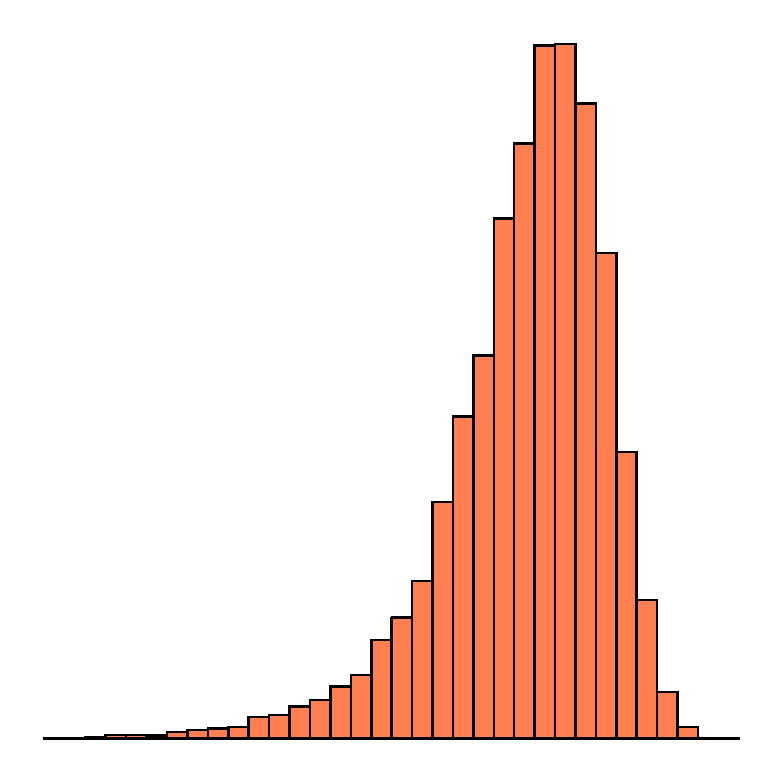
\includegraphics[scale=0.4]{img/descriptive/histograma_asimetrico_izquierda.eps}}
% \psline[linewidth=15pt,linecolor=royalblue1,arrowlength=1,arrowinset=0]{->}(5,3)(7,3)
% \rput(6,3){$Y=X^2$}
% \rput[l](7,3){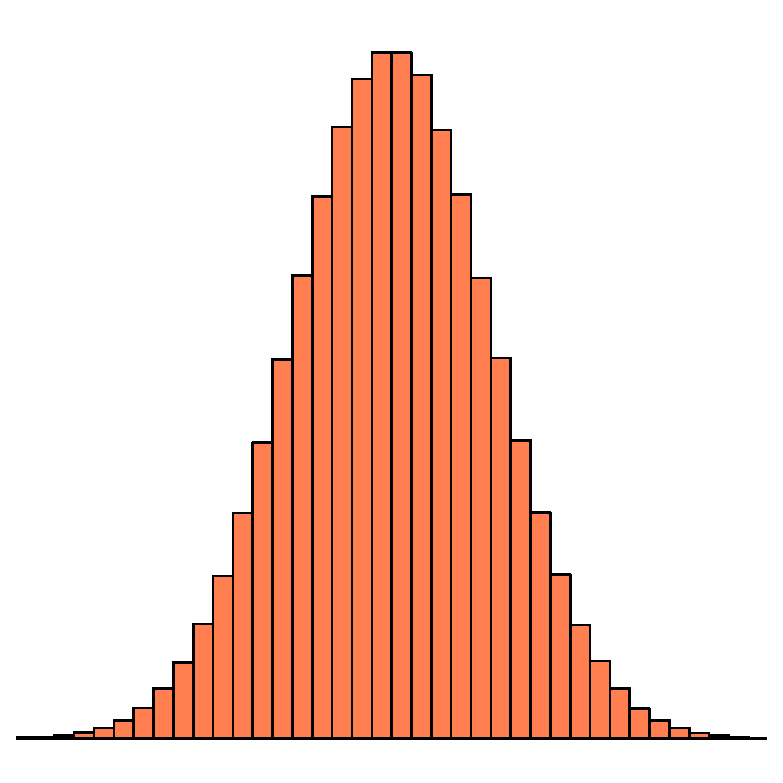
\includegraphics[scale=0.4]{img/descriptive/histograma_simetrico.eps}}
% \end{pspicture}}
% \end{center}
% 
% \note{Otras transformaciones no lineales que son habituales para corregir anormalidades de la muestra son el cuadrado, que comprime la
% escala para valores pequeños y la expande para valores altos, de manera que es muy útil para corregir asimetrías hacia la izquierda, tal y
% como puede apreciarse en estos histogramas.
% }
% \end{frame}
% 
% 
% %---------------------------------------------------------------------slide----
% \begin{frame}
% \frametitle{Transformaciones no lineales}
% Las transformaciones $Y=\sqrt x$, $Y= \log X$ y $Y=1/X$ comprimen la escala para valores altos y la expanden para valores pequeños, de manera que son útiles para corregir asimetrías hacia la
% derecha.
% \begin{center}
% \scalebox{1}{
% \begin{pspicture}(0,0)(12,6)
% \rput[l](0,3){\reflectbox{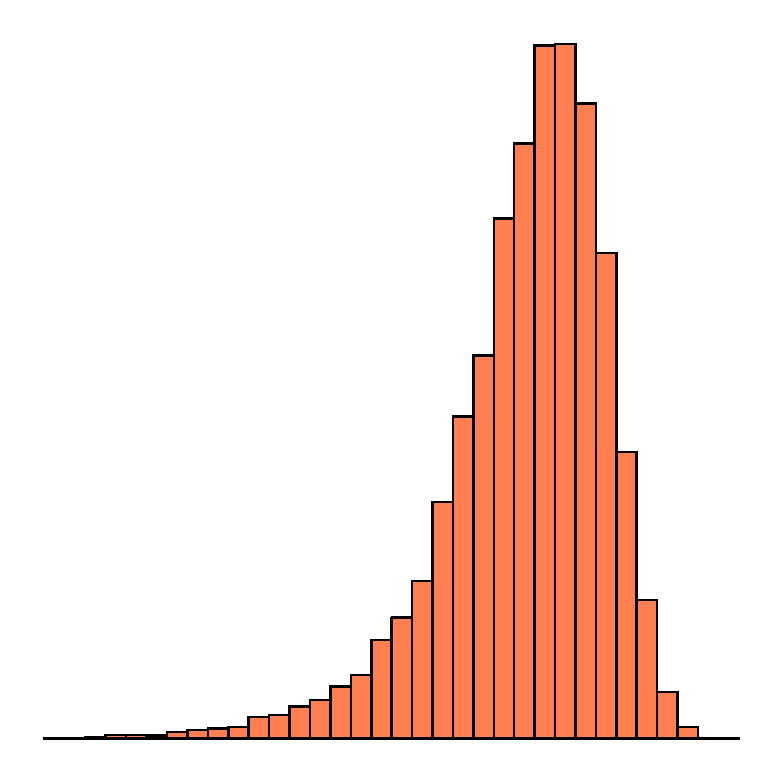
\includegraphics[scale=0.4]{img/descriptive/histograma_asimetrico_izquierda.eps}}}
% \psline[linewidth=15pt,linecolor=royalblue1,arrowlength=1,arrowinset=0]{->}(5,3)(7,3)
% \rput(6,3){$Y=\sqrt{X}$}
% \rput[l](7,3){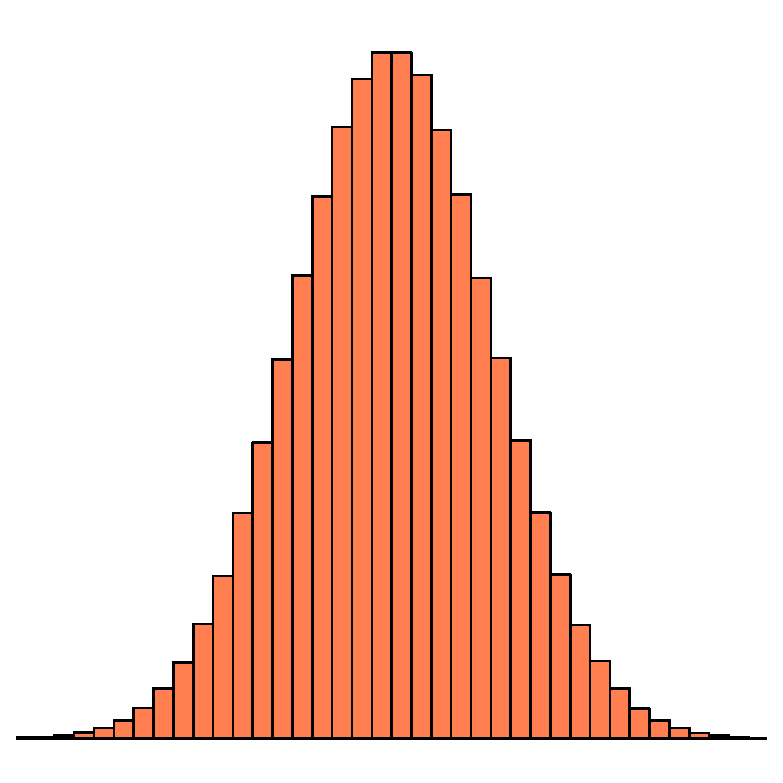
\includegraphics[scale=0.4]{img/descriptive/histograma_simetrico.eps}}
% \end{pspicture}}
% \end{center}
% 
% \note{Mientras que para corregir asimetrías hacia la derecha se utilizan o bien la raíz cuadrada, la función logarítmica o la inversa, ya
% que ambas comprimen la escala para valores altos y la expanden para valores pequeños.}
% \end{frame}
% 
% 


% %---------------------------------------------------------------------slide----
% \begin{frame}
% \frametitle{Factors}
% Sometimes is interesting to describe the frequency distribution of the main variable for different subsamples
% corresponding to the categories of another variable that is known as \structure{\textbf{classificatory variable}} or
% \structure{\textbf{factor}}.
% 
% \structure{Example} Dividing the sample of heights by sex we get two subsamples
% \begin{center}
% \begin{tabular}{lll}
% \hline
% \multirow{2}{*}{Women} &
% 173, 158, 174, 166, 162, 177, 165, 154, 166, 182, \\
% & 169, 172, 170, 168. \\
% \hline
% \multirow{2}{*}{Men} &
% 179, 181, 172, 194, 185, 187, 198, 178, 188, 171,\\
% & 175, 167, 186, 172, 176, 187. \\
% \hline
% \end{tabular}
% \end{center}
% \end{frame}
% 
% 
% %---------------------------------------------------------------------slide----
% \begin{frame}
% \frametitle{Comparing distributions for the levels of a factor }
% 
% \begin{center}
% \scalebox{0.5\textwidth}{% Created by tikzDevice version 0.8.1 on 2016-01-28 18:44:16
% !TEX encoding = UTF-8 Unicode
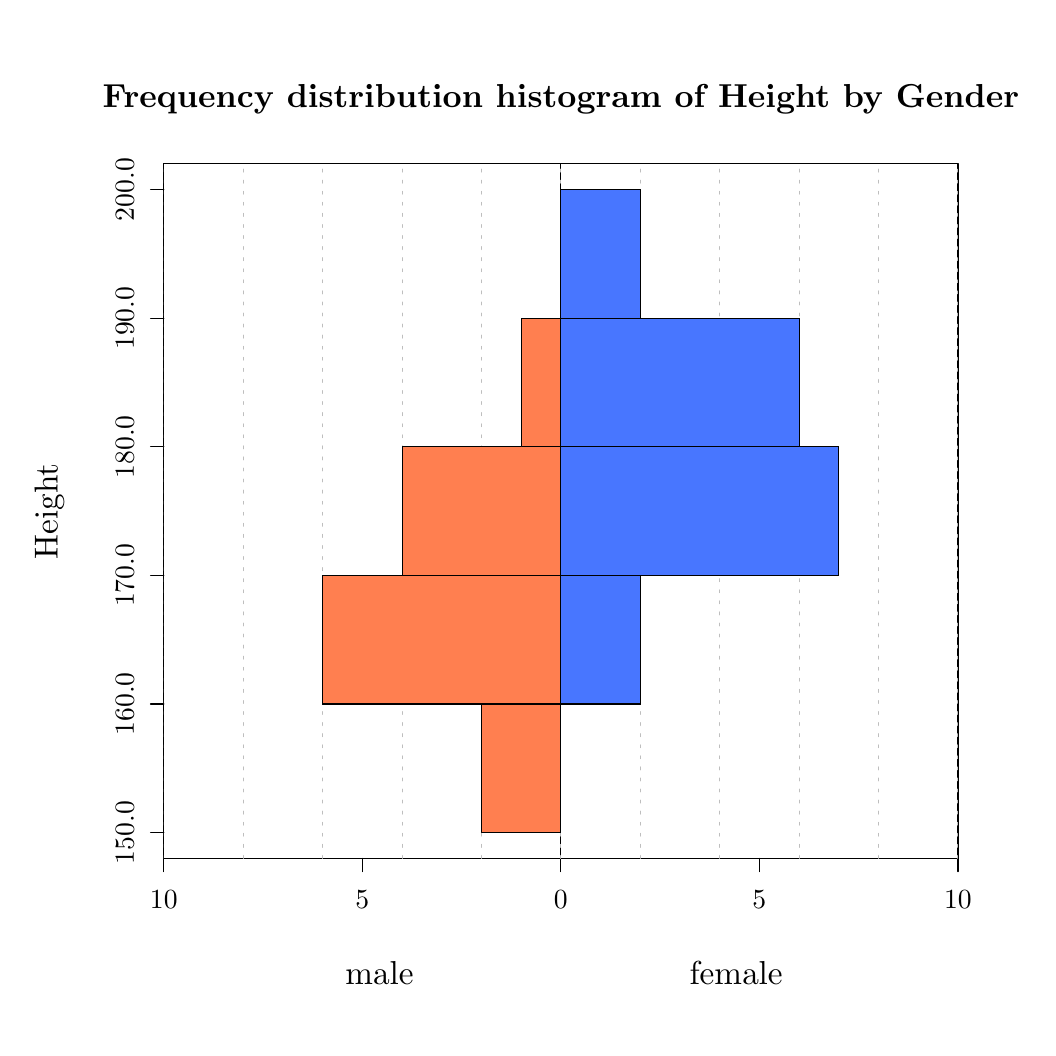
\begin{tikzpicture}[x=1pt,y=1pt]
\definecolor{fillColor}{RGB}{255,255,255}
\path[use as bounding box,fill=fillColor,fill opacity=0.00] (0,0) rectangle (361.35,361.35);
\begin{scope}
\path[clip] (  0.00,  0.00) rectangle (361.35,361.35);
\definecolor{drawColor}{RGB}{0,0,0}

\path[draw=drawColor,line width= 0.4pt,line join=round,line cap=round] (192.68, 70.49) rectangle (163.98,116.97);

\path[draw=drawColor,line width= 0.4pt,line join=round,line cap=round] (192.68,116.97) rectangle (106.59,163.44);

\path[draw=drawColor,line width= 0.4pt,line join=round,line cap=round] (192.68,163.44) rectangle (135.28,209.91);

\path[draw=drawColor,line width= 0.4pt,line join=round,line cap=round] (192.68,209.91) rectangle (178.33,256.38);

\path[draw=drawColor,line width= 0.4pt,line join=round,line cap=round] (192.68,256.38) rectangle (192.68,302.86);

\end{scope}
\begin{scope}
\path[clip] (  0.00,  0.00) rectangle (361.35,361.35);
\definecolor{drawColor}{RGB}{0,0,0}

\path[draw=drawColor,line width= 0.4pt,line join=round,line cap=round] (192.68, 70.49) rectangle (192.68,116.97);

\path[draw=drawColor,line width= 0.4pt,line join=round,line cap=round] (192.68,116.97) rectangle (221.37,163.44);

\path[draw=drawColor,line width= 0.4pt,line join=round,line cap=round] (192.68,163.44) rectangle (293.11,209.91);

\path[draw=drawColor,line width= 0.4pt,line join=round,line cap=round] (192.68,209.91) rectangle (278.76,256.38);

\path[draw=drawColor,line width= 0.4pt,line join=round,line cap=round] (192.68,256.38) rectangle (221.37,302.86);

\node[text=drawColor,anchor=base,inner sep=0pt, outer sep=0pt, scale=  1.20] at (192.68,332.61) {\bfseries Frequency distribution histogram of Height by Gender};
\end{scope}
\begin{scope}
\path[clip] (  0.00,  0.00) rectangle (361.35,361.35);
\definecolor{drawColor}{RGB}{0,0,0}

\path[draw=drawColor,line width= 0.4pt,line join=round,line cap=round] ( 49.20, 61.20) -- (336.15, 61.20);

\path[draw=drawColor,line width= 0.4pt,line join=round,line cap=round] ( 49.20, 61.20) -- ( 49.20, 56.40);

\path[draw=drawColor,line width= 0.4pt,line join=round,line cap=round] (120.94, 61.20) -- (120.94, 56.40);

\path[draw=drawColor,line width= 0.4pt,line join=round,line cap=round] (192.68, 61.20) -- (192.68, 56.40);

\path[draw=drawColor,line width= 0.4pt,line join=round,line cap=round] (264.41, 61.20) -- (264.41, 56.40);

\path[draw=drawColor,line width= 0.4pt,line join=round,line cap=round] (336.15, 61.20) -- (336.15, 56.40);

\node[text=drawColor,anchor=base,inner sep=0pt, outer sep=0pt, scale=  1.00] at ( 49.20, 43.20) {10};

\node[text=drawColor,anchor=base,inner sep=0pt, outer sep=0pt, scale=  1.00] at (120.94, 43.20) { 5};

\node[text=drawColor,anchor=base,inner sep=0pt, outer sep=0pt, scale=  1.00] at (192.68, 43.20) { 0};

\node[text=drawColor,anchor=base,inner sep=0pt, outer sep=0pt, scale=  1.00] at (264.41, 43.20) { 5};

\node[text=drawColor,anchor=base,inner sep=0pt, outer sep=0pt, scale=  1.00] at (336.15, 43.20) {10};

\path[draw=drawColor,line width= 0.4pt,line join=round,line cap=round] ( 49.20, 70.49) -- ( 49.20,302.86);

\path[draw=drawColor,line width= 0.4pt,line join=round,line cap=round] ( 49.20, 70.49) -- ( 44.40, 70.49);

\path[draw=drawColor,line width= 0.4pt,line join=round,line cap=round] ( 49.20,116.97) -- ( 44.40,116.97);

\path[draw=drawColor,line width= 0.4pt,line join=round,line cap=round] ( 49.20,163.44) -- ( 44.40,163.44);

\path[draw=drawColor,line width= 0.4pt,line join=round,line cap=round] ( 49.20,209.91) -- ( 44.40,209.91);

\path[draw=drawColor,line width= 0.4pt,line join=round,line cap=round] ( 49.20,256.38) -- ( 44.40,256.38);

\path[draw=drawColor,line width= 0.4pt,line join=round,line cap=round] ( 49.20,302.86) -- ( 44.40,302.86);

\node[text=drawColor,rotate= 90.00,anchor=base,inner sep=0pt, outer sep=0pt, scale=  1.00] at ( 38.40, 70.49) {150.0};

\node[text=drawColor,rotate= 90.00,anchor=base,inner sep=0pt, outer sep=0pt, scale=  1.00] at ( 38.40,116.97) {160.0};

\node[text=drawColor,rotate= 90.00,anchor=base,inner sep=0pt, outer sep=0pt, scale=  1.00] at ( 38.40,163.44) {170.0};

\node[text=drawColor,rotate= 90.00,anchor=base,inner sep=0pt, outer sep=0pt, scale=  1.00] at ( 38.40,209.91) {180.0};

\node[text=drawColor,rotate= 90.00,anchor=base,inner sep=0pt, outer sep=0pt, scale=  1.00] at ( 38.40,256.38) {190.0};

\node[text=drawColor,rotate= 90.00,anchor=base,inner sep=0pt, outer sep=0pt, scale=  1.00] at ( 38.40,302.86) {200.0};
\end{scope}
\begin{scope}
\path[clip] (  0.00,  0.00) rectangle (361.35,361.35);
\definecolor{drawColor}{RGB}{0,0,0}

\node[text=drawColor,anchor=base,inner sep=0pt, outer sep=0pt, scale=  1.20] at (127.10, 15.60) {male};

\node[text=drawColor,anchor=base east,inner sep=0pt, outer sep=0pt, scale=  1.20] at (272.83, 15.60) {female};

\node[text=drawColor,rotate= 90.00,anchor=base,inner sep=0pt, outer sep=0pt, scale=  1.20] at ( 10.80,186.67) {Height};
\end{scope}
\begin{scope}
\path[clip] ( 49.20, 61.20) rectangle (336.15,312.15);
\definecolor{drawColor}{RGB}{0,0,0}

\path[draw=drawColor,line width= 0.4pt,line join=round,line cap=round] (192.68, 61.20) -- (192.68,312.15);
\end{scope}
\begin{scope}
\path[clip] (  0.00,  0.00) rectangle (361.35,361.35);
\definecolor{drawColor}{RGB}{0,0,0}

\path[draw=drawColor,line width= 0.4pt,line join=round,line cap=round] ( 49.20, 61.20) --
	(336.15, 61.20) --
	(336.15,312.15) --
	( 49.20,312.15) --
	( 49.20, 61.20);
\end{scope}
\begin{scope}
\path[clip] ( 49.20, 61.20) rectangle (336.15,312.15);
\definecolor{drawColor}{RGB}{190,190,190}

\path[draw=drawColor,line width= 0.4pt,dash pattern=on 1pt off 3pt ,line join=round,line cap=round] ( 20.51, 61.20) -- ( 20.51,312.15);

\path[draw=drawColor,line width= 0.4pt,dash pattern=on 1pt off 3pt ,line join=round,line cap=round] ( 49.20, 61.20) -- ( 49.20,312.15);

\path[draw=drawColor,line width= 0.4pt,dash pattern=on 1pt off 3pt ,line join=round,line cap=round] ( 77.90, 61.20) -- ( 77.90,312.15);

\path[draw=drawColor,line width= 0.4pt,dash pattern=on 1pt off 3pt ,line join=round,line cap=round] (106.59, 61.20) -- (106.59,312.15);

\path[draw=drawColor,line width= 0.4pt,dash pattern=on 1pt off 3pt ,line join=round,line cap=round] (135.28, 61.20) -- (135.28,312.15);

\path[draw=drawColor,line width= 0.4pt,dash pattern=on 1pt off 3pt ,line join=round,line cap=round] (163.98, 61.20) -- (163.98,312.15);

\path[draw=drawColor,line width= 0.4pt,dash pattern=on 1pt off 3pt ,line join=round,line cap=round] (192.68, 61.20) -- (192.68,312.15);

\path[draw=drawColor,line width= 0.4pt,dash pattern=on 1pt off 3pt ,line join=round,line cap=round] (221.37, 61.20) -- (221.37,312.15);

\path[draw=drawColor,line width= 0.4pt,dash pattern=on 1pt off 3pt ,line join=round,line cap=round] (250.06, 61.20) -- (250.06,312.15);

\path[draw=drawColor,line width= 0.4pt,dash pattern=on 1pt off 3pt ,line join=round,line cap=round] (278.76, 61.20) -- (278.76,312.15);

\path[draw=drawColor,line width= 0.4pt,dash pattern=on 1pt off 3pt ,line join=round,line cap=round] (307.45, 61.20) -- (307.45,312.15);

\path[draw=drawColor,line width= 0.4pt,dash pattern=on 1pt off 3pt ,line join=round,line cap=round] (336.15, 61.20) -- (336.15,312.15);
\end{scope}
\begin{scope}
\path[clip] (  0.00,  0.00) rectangle (361.35,361.35);
\definecolor{drawColor}{RGB}{0,0,0}
\definecolor{fillColor}{RGB}{255,127,80}

\path[draw=drawColor,line width= 0.4pt,line join=round,line cap=round,fill=fillColor] (192.68, 70.49) rectangle (163.98,116.97);

\path[draw=drawColor,line width= 0.4pt,line join=round,line cap=round,fill=fillColor] (192.68,116.97) rectangle (106.59,163.44);

\path[draw=drawColor,line width= 0.4pt,line join=round,line cap=round,fill=fillColor] (192.68,163.44) rectangle (135.28,209.91);

\path[draw=drawColor,line width= 0.4pt,line join=round,line cap=round,fill=fillColor] (192.68,209.91) rectangle (178.33,256.38);

\path[draw=drawColor,line width= 0.4pt,line join=round,line cap=round,fill=fillColor] (192.68,256.38) rectangle (192.68,302.86);
\definecolor{fillColor}{RGB}{72,118,255}

\path[draw=drawColor,line width= 0.4pt,line join=round,line cap=round,fill=fillColor] (192.68, 70.49) rectangle (192.68,116.97);

\path[draw=drawColor,line width= 0.4pt,line join=round,line cap=round,fill=fillColor] (192.68,116.97) rectangle (221.37,163.44);

\path[draw=drawColor,line width= 0.4pt,line join=round,line cap=round,fill=fillColor] (192.68,163.44) rectangle (293.11,209.91);

\path[draw=drawColor,line width= 0.4pt,line join=round,line cap=round,fill=fillColor] (192.68,209.91) rectangle (278.76,256.38);

\path[draw=drawColor,line width= 0.4pt,line join=round,line cap=round,fill=fillColor] (192.68,256.38) rectangle (221.37,302.86);
\end{scope}
\end{tikzpicture}
}
% \quad
% \scalebox{0.5\textwidth}{% Created by tikzDevice version 0.8.1 on 2016-01-28 18:51:29
% !TEX encoding = UTF-8 Unicode
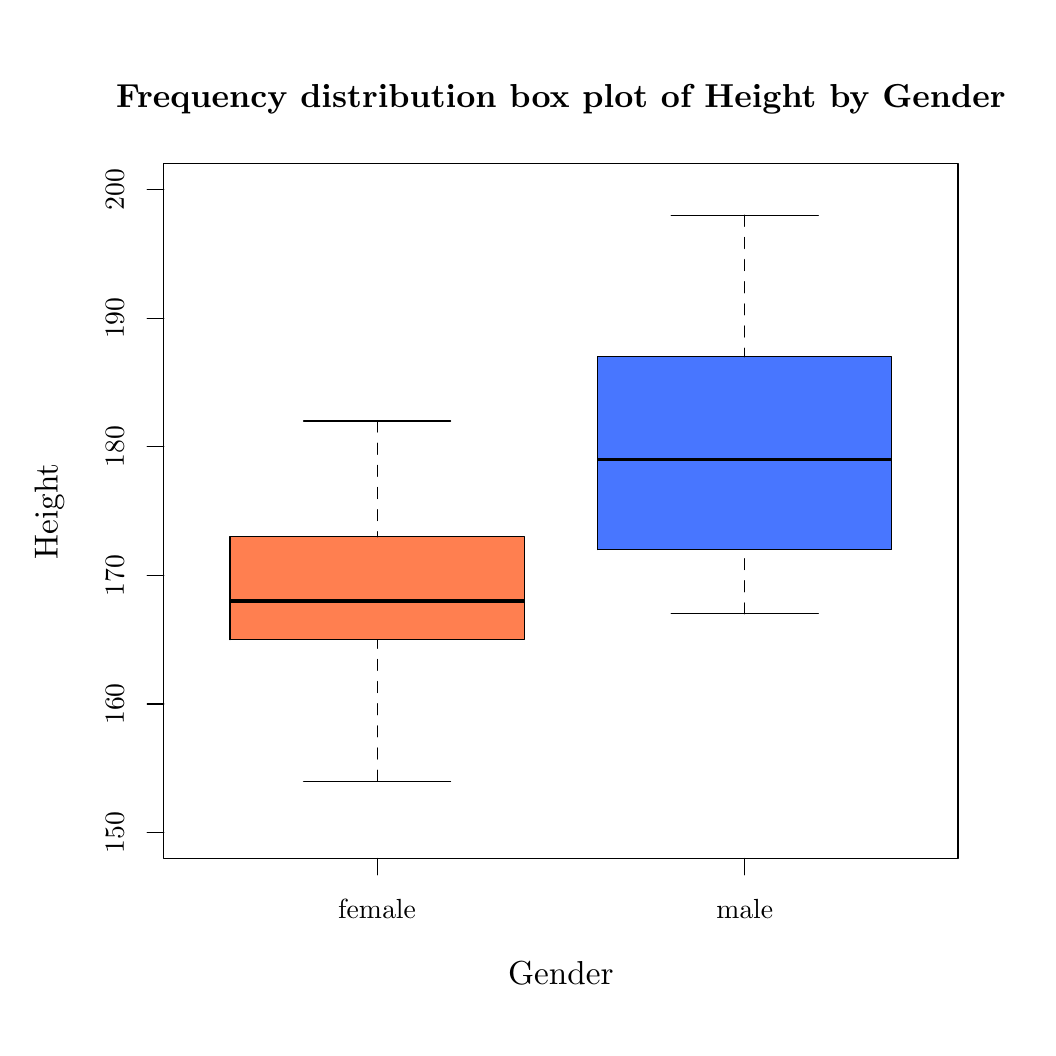
\begin{tikzpicture}[x=1pt,y=1pt]
\definecolor{fillColor}{RGB}{255,255,255}
\path[use as bounding box,fill=fillColor,fill opacity=0.00] (0,0) rectangle (361.35,361.35);
\begin{scope}
\path[clip] ( 49.20, 61.20) rectangle (336.15,312.15);
\definecolor{fillColor}{RGB}{255,127,80}

\path[fill=fillColor] ( 73.11,140.20) --
	(179.39,140.20) --
	(179.39,177.38) --
	( 73.11,177.38) --
	cycle;
\definecolor{drawColor}{RGB}{0,0,0}

\path[draw=drawColor,line width= 1.2pt,line join=round] ( 73.11,154.14) -- (179.39,154.14);

\path[draw=drawColor,line width= 0.4pt,dash pattern=on 4pt off 4pt ,line join=round,line cap=round] (126.25, 89.08) -- (126.25,140.20);

\path[draw=drawColor,line width= 0.4pt,dash pattern=on 4pt off 4pt ,line join=round,line cap=round] (126.25,219.21) -- (126.25,177.38);

\path[draw=drawColor,line width= 0.4pt,line join=round,line cap=round] ( 99.68, 89.08) -- (152.82, 89.08);

\path[draw=drawColor,line width= 0.4pt,line join=round,line cap=round] ( 99.68,219.21) -- (152.82,219.21);

\path[draw=drawColor,line width= 0.4pt,line join=round,line cap=round] ( 73.11,140.20) --
	(179.39,140.20) --
	(179.39,177.38) --
	( 73.11,177.38) --
	( 73.11,140.20);
\definecolor{fillColor}{RGB}{72,118,255}

\path[fill=fillColor] (205.96,172.73) --
	(312.24,172.73) --
	(312.24,242.44) --
	(205.96,242.44) --
	cycle;

\path[draw=drawColor,line width= 1.2pt,line join=round] (205.96,205.26) -- (312.24,205.26);

\path[draw=drawColor,line width= 0.4pt,dash pattern=on 4pt off 4pt ,line join=round,line cap=round] (259.10,149.50) -- (259.10,172.73);

\path[draw=drawColor,line width= 0.4pt,dash pattern=on 4pt off 4pt ,line join=round,line cap=round] (259.10,293.56) -- (259.10,242.44);

\path[draw=drawColor,line width= 0.4pt,line join=round,line cap=round] (232.53,149.50) -- (285.67,149.50);

\path[draw=drawColor,line width= 0.4pt,line join=round,line cap=round] (232.53,293.56) -- (285.67,293.56);

\path[draw=drawColor,line width= 0.4pt,line join=round,line cap=round] (205.96,172.73) --
	(312.24,172.73) --
	(312.24,242.44) --
	(205.96,242.44) --
	(205.96,172.73);
\end{scope}
\begin{scope}
\path[clip] (  0.00,  0.00) rectangle (361.35,361.35);
\definecolor{drawColor}{RGB}{0,0,0}

\path[draw=drawColor,line width= 0.4pt,line join=round,line cap=round] (126.25, 61.20) -- (259.10, 61.20);

\path[draw=drawColor,line width= 0.4pt,line join=round,line cap=round] (126.25, 61.20) -- (126.25, 55.20);

\path[draw=drawColor,line width= 0.4pt,line join=round,line cap=round] (259.10, 61.20) -- (259.10, 55.20);

\node[text=drawColor,anchor=base,inner sep=0pt, outer sep=0pt, scale=  1.00] at (126.25, 39.60) {female};

\node[text=drawColor,anchor=base,inner sep=0pt, outer sep=0pt, scale=  1.00] at (259.10, 39.60) {male};

\path[draw=drawColor,line width= 0.4pt,line join=round,line cap=round] ( 49.20, 70.49) -- ( 49.20,302.86);

\path[draw=drawColor,line width= 0.4pt,line join=round,line cap=round] ( 49.20, 70.49) -- ( 43.20, 70.49);

\path[draw=drawColor,line width= 0.4pt,line join=round,line cap=round] ( 49.20,116.97) -- ( 43.20,116.97);

\path[draw=drawColor,line width= 0.4pt,line join=round,line cap=round] ( 49.20,163.44) -- ( 43.20,163.44);

\path[draw=drawColor,line width= 0.4pt,line join=round,line cap=round] ( 49.20,209.91) -- ( 43.20,209.91);

\path[draw=drawColor,line width= 0.4pt,line join=round,line cap=round] ( 49.20,256.38) -- ( 43.20,256.38);

\path[draw=drawColor,line width= 0.4pt,line join=round,line cap=round] ( 49.20,302.86) -- ( 43.20,302.86);

\node[text=drawColor,rotate= 90.00,anchor=base,inner sep=0pt, outer sep=0pt, scale=  1.00] at ( 34.80, 70.49) {150};

\node[text=drawColor,rotate= 90.00,anchor=base,inner sep=0pt, outer sep=0pt, scale=  1.00] at ( 34.80,116.97) {160};

\node[text=drawColor,rotate= 90.00,anchor=base,inner sep=0pt, outer sep=0pt, scale=  1.00] at ( 34.80,163.44) {170};

\node[text=drawColor,rotate= 90.00,anchor=base,inner sep=0pt, outer sep=0pt, scale=  1.00] at ( 34.80,209.91) {180};

\node[text=drawColor,rotate= 90.00,anchor=base,inner sep=0pt, outer sep=0pt, scale=  1.00] at ( 34.80,256.38) {190};

\node[text=drawColor,rotate= 90.00,anchor=base,inner sep=0pt, outer sep=0pt, scale=  1.00] at ( 34.80,302.86) {200};
\end{scope}
\begin{scope}
\path[clip] (  0.00,  0.00) rectangle (361.35,361.35);
\definecolor{drawColor}{RGB}{0,0,0}

\node[text=drawColor,anchor=base,inner sep=0pt, outer sep=0pt, scale=  1.20] at (192.68,332.61) {\bfseries Frequency distribution box plot of Height by Gender};

\node[text=drawColor,anchor=base,inner sep=0pt, outer sep=0pt, scale=  1.20] at (192.68, 15.60) {Gender};

\node[text=drawColor,rotate= 90.00,anchor=base,inner sep=0pt, outer sep=0pt, scale=  1.20] at ( 10.80,186.68) {Height};
\end{scope}
\begin{scope}
\path[clip] (  0.00,  0.00) rectangle (361.35,361.35);
\definecolor{drawColor}{RGB}{0,0,0}

\path[draw=drawColor,line width= 0.4pt,line join=round,line cap=round] ( 49.20, 61.20) --
	(336.15, 61.20) --
	(336.15,312.15) --
	( 49.20,312.15) --
	( 49.20, 61.20);
\end{scope}
\end{tikzpicture}
}
% \end{center}
% \end{frame}
